\documentclass[11 pt]{article}
\usepackage[margin=1in]{geometry}
\usepackage{bm}
\usepackage{array,booktabs}
\usepackage{lscape}
\usepackage{setspace}
\usepackage{comment}
\usepackage{mathtools}
\usepackage{amsmath}
\usepackage{booktabs,tabularx}
\usepackage{threeparttable}
\usepackage{multirow}
\usepackage{indentfirst}
\usepackage{float}
\usepackage{amssymb}
\usepackage{hyperref}
\usepackage{natbib}
\usepackage{color}
\usepackage[justification=centering]{caption}
\usepackage[format=hang,singlelinecheck=0,font={sf,small},labelfont=bf]{subfig}
\usepackage[noabbrev]{cleveref}
\usepackage{graphicx,rotating,booktabs}
\hypersetup{
    pdfborder = {0 0 0}
}
\usepackage{afterpage}
\usepackage{amsthm}
\usepackage{siunitx}

% Diagram packages retained from the template.
\usepackage{tikz}
\usetikzlibrary{positioning}
\usetikzlibrary{arrows}

% Template font setup (Times-style text).
\usepackage{pslatex}
\usepackage[T1]{fontenc}
\usepackage[utf8]{inputenc}
\usepackage{xurl}

% Template citation/link appearance.
\definecolor{darkblue}{rgb}{0,0,.4}
\hypersetup{colorlinks=true, breaklinks=true, citecolor=darkblue, linkcolor=darkblue, menucolor=darkblue, urlcolor=darkblue}

\newcolumntype{L}[1]{>{\raggedright\let\newline\\\arraybackslash\hspace{0pt}}m{#1}}
\newcolumntype{C}[1]{>{\centering\let\newline\\\arraybackslash\hspace{0pt}}m{#1}}
\newcolumntype{R}[1]{>{\raggedleft\let\newline\\\arraybackslash\hspace{0pt}}m{#1}}

% Theorem setup follows the template; Prediction is needed by this manuscript.
\newtheorem{theorem}{Theorem}
\newtheorem{proposition}{Proposition}
\newtheorem{lemma}{Lemma}
\newtheorem{corollary}{Corollary}
\newtheorem{prediction}{Prediction}

% Manuscript-specific helper for unnumbered figure/table notes.
\newcommand\fnote[1]{\captionsetup{font=footnotesize}\caption*{#1}}

%%%%%%%%%%%%%%%%%%%%%%%%%%%%%%%%%%%%%%%%%%%%%%%%%%%%%%%%%%%%%%%%%%%%%%%%%%%%%%%%%%%%%%%%%%%%%%%%%%%%%%%%%%%%%%%%%%%%%%%%%%%%

\title{\Large The Effect of Purchase Intention Interruption on Novelty-Seeking: \\
Evidence from a Large Coffee Chain\footnote{This project is funded by Hong Kong RGC Grant \#16506525}}
\author{Francesco Gabriele\thanks{Department of Marketing, Hong Kong University of Science and Technology.} \quad Tao Li \footnotemark[2] \quad Chen Lin\thanks{Department of Marketing, Fudan University.} \quad Mengze Shi \footnotemark[2] \quad\thanks{Authors are ordered alphabetically}}
\date{\today}

\begin{document}

% Spacing and title follow the template.
\maketitle
\doublespacing

\setcounter{page}{0}
\pagenumbering{arabic}

\begin{abstract}
    \tiny \renewcommand{\baselinestretch}{1.2} \normalsize
    \singlespacing
    \noindent
    As product innovation has become a required competitive advantage for firms, understanding the driver of consumers' willingness to explore is crucial for new production diffusion. This paper asks how an unexpectedly blocked purchase affects consumers' subsequent novelty-seeking behavior. We study this question using 18 temporary exogenous store closures at a large digital coffee retailer. Because the same closure is more likely to interrupt an intended purchase for some consumers than for others, we use pre-closure behavior to predict each consumer's purchase intention during the closure and estimate a triple-differences design comparing high- and low-predicted-intention consumers. Our main finding concerns product exploration. We find that purchase interruption reduces subsequent novelty-seeking, defined as the share of distinct products purchased that the consumer has not purchased before, by 4.15 percentage points, or 8.3\% of the pre-period mean. An alternative measure based on recently introduced products yields a nearly identical 4.17-percentage-point reduction. Consistent with an interrupted purchase goal triggering counterfactual thinking and increasing the salience of familiar choices, the decline in exploration is also stronger among consumers with lower baseline novelty-seeking. More broadly, these findings show that supply interruptions can reduce consumers' receptivity to innovation even after access is restored, implying that firms can improve product-launch targeting, recommendations, and promotional incentives by accounting for whether consumers' likely purchases were recently interrupted.

    \par\smallskip
    \noindent \textbf{Keywords}: Novelty Seeking, Purchase Interruption, Triple-Difference, Counterfactual Thinking, Goal Persistence
\end{abstract}

\thispagestyle{empty}
\newpage
\setcounter{page}{1}

\section{Introduction}
\label{section:Introduction}

Ed Sander, a Dutch technology analyst who frequently travels to China, recalled his first impression of a Mascarpone Cheese Latte offered by Luckin Coffee: ``It had like the slightly salty, but cheesy kind of flavor to it, on paper it tasted quite awful. But it tasted amazing.'' Sander later posted on X that he was going ``cold turkey from the Mascarpone Cheese Latte I've been having daily when I'm in China.'' One year later, he was still mourning the drink \citep{emont2025coffeewar}. Sander is not alone in a world with continual experimentation and product innovation. Luckin, the market leader, opened 6,000 new stores and introduced 119 new products in 2024 alone, although some of the flavor combinations being developed are described by a Colombia coffee consultant as ``heresy'' by the standards of his native Colombia \citep{emont2025coffeewar}. To catch up the competitive advantage, Starbucks introduced 78 new beverages in China, 2024 \citep{chinadaily2026starbucks}. In fast food, Taco Bell tests hundreds of ideas each year and uses limited-time offers to keep menus and apps populated with new items that can bring customers back; products that take years to develop may remain on the menu for just four to six weeks \citep{haddon2025tacobell}.

Product innovation, however, is not self-executing. With a frequent menu shift and a large assortment, firms need consumers to depart from familiar choices and try something new. At the same time, frequent product changes create a common problem to consumers of losing access to their routine of familiar choices, a scenario that could also be caused by inventory shortage or store closure. The supply interruption may not only affect whether consumers come back again, but also their new product adoption behavior in the future, which has already been proved to vary with marketing strategy, market conditions, and consumer characteristics \citep{steenkamp2003trial}. Understanding the impact of supply interruption on consumers' novelty-seeking behavior and its underlying mechanism is thus managerially relevant and important for firms to better conduct product launches \citep{talay2024recession,ward2025recession} and design related marketing strategies such as new product notification and coupon issuing.

In this paper, we ask: What happens to consumers' willingness to explore when a purchase they likely intended to make is unexpectedly blocked? This question speaks directly to the tension described above: when firms continuously introduce new products while consumers simultaneously develop routines around familiar choices, an interruption to an intended purchase may alter consumers' subsequent receptivity to novelty. Answering this question, however, poses two main empirical challenges. First, purchase intention is inherently unobserved when no purchase occurs: a consumer who had no intention to purchase and a consumer whose intended purchase was blocked both leave the same observational outcome of no transaction, making it difficult to distinguish these two. Second, identifying the subsequent impact on novelty-seeking requires longitudinal observational data that follow consumers before and after such an interruption, while market conditions evolve simultaneously over time. Firms expand their store networks, product assortments change, and new products are continuously introduced, all of which can independently affect consumers' opportunities and incentives to explore. Addressing these challenges therefore requires a way to identify consumers who were likely to purchase, together with an external disruption that prevents some of these consumers from completing their intended purchases.

We study this question in a setting of a large Chinese quick-service coffee chain whose consumers order through a mobile application for pickup or delivery. The chain offers a broad and frequently changing menu, creating repeated opportunities to choose between familiar and unfamiliar products. Our data contain 7.3 million orders from 779,744 consumers at 260 stores between June 1, 2020 and December 31, 2021. The empirical exogenous variation comes from 18 temporary store closures lasting 10 to 29 days during COVID-19-related lockdowns. Similar shocks have also been leveraged by prior literature \citep{seenivasan2016store,levine2023state,ye2025close}. However, in our context, the temporary store closures are accompanied with other changes happened simultaneously, such as menu change, or post-opening marketing activities like coupon issuing or push notification. As a result, we are not interested in the causal impact of the temporary store closure per se. The same closure exposes many consumers to a supply disruption, but it is much more likely to \textit{interrupt a purchase} for consumers who otherwise would have purchased during the closure window. Using only pre-closure behavior, we predict each consumer's purchase propensity during that window and compare consumers with high versus low predicted purchase intention in a triple-differences design. Rather than treating the closures as the object of study, we use them to separate general disruption exposure from the \textit{incremental effect of an intended but unrealized purchase}. This approach complements recent work that uses hurricane-induced stockouts and temporary store disruptions as exogenous changes in choice opportunities to study persistence in realized brand and store choices \citep{levine2023state,Levine2026}.

We find that interrupting a likely purchase substantially narrows subsequent product exploration. We measure novelty-seeking as the share of distinct products purchased in a period that the consumer has not purchased before. Relative to consumers with low predicted purchase intention, consumers whose purchases were more likely to be interrupted exhibit a 4.15-percentage-point lower post-reopening response in novelty-seeking, equivalent to 8.3\% of the pre-period mean. The result is nearly identical when we define exploration using recently introduced products: the corresponding reduction in new-product-seeking is 4.17 percentage points. We interpret the pattern through familiar-choice salience: an interrupted purchase leaves a counterfactual thinking of the potential purchase if there were no interruption and a salient representation of the unfinished goal; when consumers get access to the purchase again, that representation can pull choice toward the familiar purchase path and away from exploration. The heterogeneity evidence further supports this interpretation. The reduction in novelty-seeking is strongest among consumers who were less exploratory before the closure: holding baseline purchase history fixed, a one-standard-deviation increase in baseline novelty-seeking makes the interruption effect 2.94 percentage points less negative. We also examine two alternative explanations: differential exposure to new-product notifications and differences in the assortments consumers encounter upon returning, and find that neither is supported by extra evidence in data.

Our results offer several managerial implications for product launch and post-disruption marketing strategies. Firms commonly evaluate product launches based on product characteristics, competitive conditions, and market-wide timing, but our findings suggest that consumers' recent purchase experiences can also shape their receptivity to new products. After a store closure, stockout, app outage, delivery suspension, or other temporary access constraint, consumers whose likely purchases were interrupted become less willing to explore unfamiliar products and more inclined toward familiar choices. Firms may therefore want to account for such heterogeneity when deciding whom to target with newly introduced products. When launch timing or targeting is flexible, early promotion of new products may be directed toward consumers whose purchases were less likely to have been interrupted, while familiar or previously purchased products can be recommended to interrupted consumers to better match their immediate preference for familiar choices. When rapid new-product diffusion is strategically important and these consumers cannot be avoided as a target segment, firms may need to provide stronger incentives, such as coupons, price promotions, or other trial inducements, to encourage them to depart from their familiar purchase path. The findings also have implications for personalized recommendation systems: rather than uniformly promoting recently introduced products after operations recover, firms can incorporate whether a consumer's likely purchase was interrupted when deciding between recommending familiar and novel products. More broadly, recovered traffic or transaction volume does not necessarily imply recovered receptivity to innovation. Firms managing disruptions should therefore consider both the level and the composition of returning demand when designing product launches, recommendations, promotions, and new-product diffusion strategies.

This paper contributes three streams of prior literature. First, we contribute to research on novelty-seeking and exploratory consumer behavior. Novelty-seeking refers to consumers' tendency to approach products or consumption experiences that are new to them and has long been viewed as an important dimension of consumer innovativeness and exploratory behavior \citep{hirschman1980innovativeness,raju1980optimum,steenkamp1992role}. This literature offers several explanations for why consumers seek novelty. Consumers may explore to obtain stimulation and satisfy curiosity \citep{raju1980optimum,steenkamp1992role}, to learn about uncertain product quality \citep{erdem1996uncertainty}, or because they differ in their underlying propensity to adopt and experiment with new products \citep{hirschman1980innovativeness,steenkamp2003trial}. Research on new-product adoption further shows that consumers' willingness to try unfamiliar products depends not only on such individual differences, but also on product perceptions, social context, and firms' marketing activities \citep{ostlund1974perceived,fisher1992investigation,steenkamp2003trial}. Closely related research on variety-seeking shows that exploratory choice is also responsive to the immediate choice environment, including prior consumption, contextual stimulation, perceived freedom, time of day, choice architecture, and active goals \citep{simonson1990variety,menon1995context,levav2009freedom,gullo2019timeofday,odonnell2023bundle,rafieian2024goals}. We extend this literature by showing that a prior purchase interruption can also shape subsequent novelty-seeking. We show that an interruption to a familiar purchase can carry over to subsequent choices and reduce consumers' willingness to discover products they have not previously purchased. Thus, novelty-seeking is shaped not only by characteristics of consumers, products, and the contemporaneous choice environment, but also by whether consumers were able to complete a purchase they previously intended to make.

Second, we contribute to research on temporary disruptions. Store closures affect sales, store switching, retention, channel use, and subsequent activity \citep{haans2010closing,seenivasan2016store,ye2025close}; stockouts and service-capacity constraints affect substitution, product choice, and later purchasing \citep{fitzsimons2000consumer,anderson2006stockouts,jing2011stockouts,che2012outofstock,wangenheim2007overbooking}. Recent work further uses temporary changes in choice opportunities to distinguish state dependence from persistent consumer heterogeneity \citep{levine2023state,Levine2026}. We shift the unit of interpretation from the disruption itself to whether the disruption \textit{binds against an active purchase intention}. That distinction allows the same exogenous supply shock to reveal a behavioral consequence that average closure effects can miss: a purchase that never occurs can nevertheless shape what consumers choose later. In this sense, the disruption is the empirical lever; the contribution is evidence that intended but unrealized consumption can leave a persistent footprint on product exploration.

Third, we provide the field evidence to research on counterfactual thinking, interrupted decisions, and goal persistence. Counterfactual thinking makes salient how an event could have unfolded differently and can guide subsequent intentions and behavior \citep{roese1994functional,epstude2008functional}. Research on consumer goals provides a complementary prediction about what happens when pursuit is interrupted: resuming an interrupted decision can shift processing toward a more goal-directed mode \citep{liu2008focusing}; a goal that has been set aside can regain influence over subsequent choice \citep{carlson2013goal}; and proximity to completing a focal goal can increase the attractiveness of returning to it \citep{jhang2015interruption}. Recent work further shows that making progress toward an explicit goal can reduce switching to alternative means by increasing the relative attractiveness of the initial means \citep{friedman2025road}. Our setting brings these ideas to naturally occurring repeated purchases. A temporary closure makes the unrealized purchase unusually easy to imagine and leaves the familiar consumption path unresolved. The main effect and the predicted heterogeneity together are consistent with the resulting familiar-choice salience carrying into subsequent marketplace choices and reducing exploration.


\section{Conceptual Motivation and Empirical Predictions}

\subsection{Behavioral Mechanism: Counterfactual Thinking and Goal Persistence}

A purchase interruption differs from simple non-purchase. A consumer who did not intend to purchase leaves no purchase goal unresolved. By contrast, when access is unexpectedly removed from a consumer who was likely to purchase, the event prevents an intended consumption episode from being completed. We propose that this unfinished episode carries into subsequent choice and changes the consumer's willingness to explore.

Counterfactual thinking and research on goal persistence explain why. Counterfactual thinking makes people represent how an event could have unfolded differently and can guide subsequent intentions and behavior \citep{epstude2008functional}. Unfulfilled goals can remain cognitively accessible \citep{masicampo2011consider}; goals that have been set aside can regain influence over later choice \citep{carlson2013goal}; and proximity to goal completion can increase the attractiveness of returning to the focal task \citep{jhang2015interruption}. In consumer settings, responses to product unavailability likewise depend on commitment to the intended option \citep{fitzsimons2000consumer}. An interrupted purchase can therefore remain psychologically active after the access constraint itself disappears.

For repeated purchases, this carryover should favor familiar choices. Consumers' routines are built around products and choice paths reinforced by prior consumption. When a likely purchase is blocked, the counterfactual representation of what would otherwise have occurred and the unresolved purchase goal both point back toward this familiar path. Once access returns, familiar products therefore become relatively more salient than unfamiliar alternatives. We refer to this response as \textit{familiar-choice salience}. Its central implication is that consumers whose likely purchases are interrupted should subsequently devote a smaller share of their choices to products they have not purchased before.

The same mechanism generates a heterogeneity prediction. Consumers with lower baseline novelty-seeking concentrate more of their observed consumption on familiar products and established routines. For these consumers, an interruption should more strongly reactivate an established familiar path. Consumers who are already highly exploratory have less concentrated familiar routines, so the same interruption should exert a weaker pull away from novelty. Baseline novelty-seeking therefore provides a natural moderator of the interruption effect.

\subsection{A Parsimonious Framework}
\label{section:Micro-Foundation}

We formalize this intuition with a reduced-form framework that maps the behavioral mechanism to the empirical design. Let $i$ index consumers and $t$ relative periods around the focal closure. Let $\text{Post}_{t}$ indicate periods after reopening, $\text{Treated}_{i}$ indicate whether the consumer is exposed to the focal store closure, and let $p_i\in[0,1]$ denote the ex-ante probability that consumer $i$ would have made a purchase during the closure window absent the closure. A larger $p_i$ means that the same closure is more likely to interrupt a purchase the consumer otherwise would have made.

Let $Y^N_{it}$ denote novelty-seeking conditional on making a purchase, and let $\vartheta_i$ summarize the consumer's underlying tendency to explore unfamiliar products. We represent expected novelty-seeking as
\begin{equation}
\mathbb{E}\left[
Y^N_{it}\mid\text{Purchase}_{it}=1
\right]
=
\mu_{it}(\vartheta_i)
-
\lambda(\vartheta_i)
\left(
\text{Post}_{t}
\times
\text{Treated}_{i}
\times
p_i
\right),
\label{eq:parsimonious_novelty_model}
\end{equation}
where $\mu_{it}(\vartheta_i)$ collects the components of expected novelty-seeking that are unrelated to the interruption-specific familiar-choice channel. The function $\lambda(\vartheta_i)$ captures the strength of familiar-choice salience generated by a likely purchase interruption. The interaction $\text{Post}_{t}\times\text{Treated}_{i}\times p_i$ is zero before the closure and for control consumers, and becomes larger after reopening for treated consumers with greater ex-ante purchase propensity. Equation~\eqref{eq:parsimonious_novelty_model} therefore isolates the behavioral component that should vary with the likelihood that the closure actually interrupted an intended purchase.

The behavioral account imposes two restrictions:
\begin{equation}
\lambda(\vartheta_i)>0,
\qquad
\lambda'(\vartheta_i)<0.
\label{eq:parsimonious_lambda}
\end{equation}
The first captures the central mechanism: a likely purchase interruption shifts subsequent choice toward familiar products and away from exploration. The second captures the predicted heterogeneity: consumers with a stronger underlying tendency to explore have a weaker familiar-choice response to the interruption. In the empirical analysis, we use consumers' baseline novelty-seeking to proxy for this underlying heterogeneity.

For treated consumers after reopening, the interruption-related component of novelty-seeking becomes more negative as purchase intention rises:
\begin{equation}
D_p(\vartheta_i)
\equiv
\frac{\partial}{\partial p_i}
\left[-\lambda(\vartheta_i)p_i\right]
=
-\lambda(\vartheta_i)
<0.
\label{eq:parsimonious_main_prediction}
\end{equation}
Here $D_p(\vartheta_i)$ is the marginal change in the interruption-related novelty response as the probability of an intended purchase rises. A negative value means that, among otherwise comparable treated consumers, a closure that is more likely to bind against an intended purchase should produce a more negative post-reopening novelty response.

\begin{prediction}[Purchase interruption reduces novelty-seeking]
Compared with consumers with lower purchase intention during the closure, consumers with higher purchase intention should exhibit a lower treated-control post-reopening response in novelty-seeking. Thus, the high-minus-low triple-differences effect on novelty-seeking should be negative.
\end{prediction}

The framework uses the continuous purchase probability $p_i$ to make the intensity of likely interruption explicit. Our main empirical specification instead classifies consumers into high- and low-predicted-intention groups. For any $p_H>p_L$, the corresponding finite-difference implication is
\begin{equation}
D(p_H,p_L;\vartheta_i)
=
-\lambda(\vartheta_i)(p_H-p_L)
<0.
\label{eq:parsimonious_binary_prediction}
\end{equation}
This expression is the discrete counterpart of equation~\eqref{eq:parsimonious_main_prediction}: moving from a lower to a higher purchase propensity makes the interruption-related response more negative by an amount proportional to $p_H-p_L$. Under the identifying conditions developed in Section~\ref{section:3.3.1}, this finite difference maps to the high-minus-low triple-differences estimand.

The second restriction generates the heterogeneity prediction:
\begin{equation}
\frac{\partial D(p_H,p_L;\vartheta_i)}
{\partial\vartheta_i}
=
-\lambda'(\vartheta_i)(p_H-p_L)
>0.
\label{eq:parsimonious_heterogeneity_prediction}
\end{equation}
Because $D(p_H,p_L;\vartheta_i)<0$, a positive derivative means that the interruption effect becomes less negative as the consumer's underlying tendency toward novelty increases.

\begin{prediction}[Baseline novelty attenuates the interruption effect]
The negative interruption-related effect on novelty-seeking should be stronger among consumers with lower baseline novelty-seeking and weaker among consumers who are already more exploratory.
\end{prediction}

Together, the two predictions organize the empirical analysis: the first tests whether a likely purchase interruption narrows subsequent exploration, and the second tests whether that narrowing is strongest when consumers' prior choices are more concentrated on familiar products.


\section{Setting and Data}
\label{section:Setting and Data}

Our setting combines three features that are particularly useful for studying purchase interruption and novelty-seeking: detailed digital purchase histories, a broad and frequently changing product menu, and temporary localized closures that sharply restrict access for a subset of consumers. We use administrative records from a large Chinese quick-service coffee chain whose consumers order primarily through a mobile application for pickup or delivery. The data cover 19 months from June 1, 2020 to December 31, 2021 and contain 7,312,498 orders, represented by 10,631,250 product-line records, from 779,744 consumers at 260 stores in a major city. For each order, we observe the consumer, purchase date, store, and products purchased. Because consumers can purchase from any store in the chain, our behavioral outcomes aggregate purchases chain-wide rather than only at the focal store.

Temporary store closures during COVID-19-related lockdowns provide the access shocks. We identify 18 closures lasting 10 to 29 days after applying the screens described in Appendix~\ref{app:closure_registry}. The novelty-seeking result remains similar when all 22 eligible closures are retained: the DDD is $-3.86$ percentage points, compared with $-4.15$ percentage points in the preferred sample (Appendix Table~\ref{tab:closure_registry_sensitivity}). For each closure event $e$, we construct four pre-closure and four post-reopening windows, each with the same length $L_e$ as the closure. Period 0 is the closure window itself. This event-based construction puts closures of different durations on a common relative-time scale and lets the pre- and post-period outcomes be measured over windows of comparable length within each event.

We assign treatment exposure through consumers' pre-closure store relationships. A consumer can purchase at multiple stores, so a store closure is most likely to represent a meaningful access shock when the closing store was central to the consumer's prior purchases. We therefore restrict attention to consumers with at least five pre-closure purchase days and define a consumer's focal store as the store accounting for at least 80\% of her pre-closure purchases. Treated consumers have a focal store that closes; control consumers have a focal store among five matched stores that remain open. For each closing store, we select without replacement the five eligible control stores with the closest setup dates. Because the firm opened stores in rollout cohorts, setup timing proxies for stores' operational status and strategic importance. We exclude university and college stores because campus lockdowns and summer departures sent many students outside the focal city, where their purchases are not observed; zero local transactions could therefore reflect population departure rather than a supply interruption. Treatment therefore captures exposure to a localized access restriction, while subsequent outcomes continue to include purchases at any store in the observed chain. The resulting sample contains 40,148 consumer-events, including 7,390 treated and 32,758 control consumers.

\subsection{Identifying Likely Purchase Interruption}
\label{section:classifier}

Closure exposure alone does not reveal whether a purchase was interrupted. A treated consumer who would not have purchased during the closure and a treated consumer who intended to purchase but was prevented from doing so both generate no focal-store transaction during the closure. The key third dimension of our design is therefore ex-ante purchase intention: among consumers exposed to the same type of closure, the interruption channel should be strongest for those who otherwise were most likely to purchase during the closure window.

We infer this latent purchase propensity using an XGBoost classifier trained exclusively on pre-closure information. The prediction target is whether a consumer makes at least one purchase at any store in the chain during a window of the same length as the focal closure. Thus, treatment is assigned through the preferred pre-closure store, whereas the classifier target and behavioral outcomes are measured chain-wide. Because the probability of at least one purchase mechanically rises with window length, we estimate a separate model for each observed closure duration. Training uses relative pre-periods $-4$ through $-2$, with predictors constructed from information available before each prediction window; relative period $-1$ is held out for validation. We also conduct an additional period-0 audit among control consumers, whose matched focal stores remain open and whose realized purchase behavior is therefore observable during the focal closure window. For treated consumers, the corresponding period-0 purchase outcome absent the closure is counterfactual, which is precisely why the predicted propensity is needed.

The predictors summarize the consumer's purchase history before the prediction window: recent purchase frequency, recency since the last purchase, total purchase history, focal-store loyalty, basket composition, discount and coupon use, day-of-week purchasing patterns, demographics, and push-notification history. The classifier produces a predicted probability between zero and one. We define $\text{High}=1$ when this predicted probability is at least 0.5 and $\text{High}=0$ otherwise. The indicator is constructed ex ante for both treated and control consumers; a likely interrupted purchase occurs when a consumer is both treated and high predicted intention.

\begin{table}[!ht]
\centering
\caption{Purchase-intention classifier performance on the final cohort}
\label{tab:classifier_diagnostics}
\small
\begin{tabularx}{\textwidth}{Xrrrrrr}
\toprule
Evaluation sample & $N$ & Prevalence & ROC-AUC & PR-AUC & Brier & Calibration slope \\
\midrule
Control, period 0 & 32,758 & .263 & .781 & .583 & .172 & .471 \\
Control, pre-period $-1$ & 32,758 & .308 & .814 & .677 & .164 & .536 \\
Treated, pre-period $-1$ & 7,390 & .314 & .818 & .697 & .162 & .537 \\
\bottomrule
\end{tabularx}
\vspace{1mm}
\fnote{Notes: All rows use the exact final 18-event cohort. Prevalence is the observed share purchasing at least once in the evaluation window. ROC-AUC measures ranking performance; PR-AUC should be compared with prevalence, the performance of an uninformative ranking. The Brier score is the mean squared probability error, for which lower values are better. The corresponding constant-prevalence Brier scores are .194, .213 and .216. Perfect calibration has intercept zero and slope one; the estimated intercepts are $-.599$, $-.309$ and $-.276$, respectively. Period-0 outcomes are not observable for treated consumers absent the closure, so that validation is conducted only among controls.}
\end{table}

Table~\ref{tab:classifier_diagnostics} shows that the model meaningfully ranks likely purchasers before the focal post-reopening outcomes are observed. The period-0 control audit is especially informative because it evaluates the prediction in the same relative window in which treated consumers face the closure. Its ROC-AUC is 0.781 and its PR-AUC is 0.583, compared with an observed purchase prevalence of 0.263. Its Brier score is 0.172, below the 0.194 score obtained by assigning every consumer the sample purchase rate. The purpose of the classifier in the design is therefore not to recover a perfectly observed psychological intention; it is to separate consumers with materially different ex-ante propensities to purchase during the window in which the access shock occurs. Appendix~\ref{app:classifier_details} reports confusion matrices, calibration, duration-specific performance, cutoff tradeoffs, and score overlap.

\subsection{Analysis Sample and Raw Closure Shock}
\label{section:statistics}

For the descriptive access-shock evidence in this section, we measure purchase frequency as the number of days with at least one purchase divided by the number of calendar days $L_e$ in the event window. This normalization makes purchase activity comparable across closure events of different durations.

The event construction yields 321,184 consumer-event-period observations for purchase activity. Novelty-seeking is defined only in windows containing at least one purchase. There are 105,854 such purchasing windows; after the consumer-event fixed-effects estimator removes consumer-events observed in only one product-choice period, the main novelty-seeking regressions use 99,644 observations. The classifier places 2,041 treated consumers, or 27.6\%, in the high-predicted-intention group.

\begin{table}[h!]
\centering
\caption{Four-cell descriptive statistics before closure}
\label{tab:treatment_control_balance}
\small
\begin{tabular}{lrrrr}
\toprule
& \multicolumn{2}{c}{Low predicted intention} & \multicolumn{2}{c}{High predicted intention} \\
\cmidrule(lr){2-3}\cmidrule(lr){4-5}
Variable & Control & Treated & Control & Treated \\
\midrule
Consumer-events & 23,934 & 5,349 & 8,824 & 2,041 \\
Predicted purchase-intention probability & .135 & .132 & .773 & .785 \\
& (.141) & (.139) & (.157) & (.158) \\
Pre-period purchase frequency & .022 & .021 & .127 & .114 \\
& (.035) & (.033) & (.116) & (.112) \\
Pre-period novelty-seeking & .604 & .602 & .450 & .498 \\
& (.392) & (.392) & (.309) & (.305) \\
consumers with at least one pre-period purchase & 12,317 & 2,745 & 8,798 & 2,034 \\
Share of pre-period windows with a purchase & .214 & .211 & .751 & .753 \\
Closure duration in days & 16.2 & 16.9 & 18.8 & 21.7 \\
& (5.6) & (6.5) & (6.4) & (7.2) \\
\bottomrule
\end{tabular}
\vspace{1mm}
\fnote{Notes: The unit is a consumer-event. Standard deviations are in parentheses. Pre-period purchase frequency is first averaged over relative periods $-4$ through $-1$ within a consumer-event. Pre-period novelty-seeking is averaged over purchasing windows and is reported for consumer-events with at least one pre-period purchase. The purchase share is the fraction of the four pre-period windows in which the consumer purchases at least one product. High and low groups differ mechanically in purchase propensity; the relevant descriptive comparison is treated versus control within each predicted-intention group. Closure duration is repeated at the consumer-event level and is shown descriptively, without consumer-level balance inference.}
\end{table}

Table~\ref{tab:treatment_control_balance} displays the four cells that form the triple-differences comparison. The classifier creates economically distinct intention groups: high-intention consumers make at least one purchase in about three quarters of their pre-period windows, compared with about one fifth for low-intention consumers. At the same time, treated and control consumers have very similar predicted purchase propensities within each intention stratum: 0.132 versus 0.135 in the low group and 0.785 versus 0.773 in the high group. The table also makes clear why the design is based on changes in treated-control gaps rather than equality of pre-period levels. Consumer-event fixed effects absorb time-invariant level differences, while the pre-period event-study tests below evaluate whether the treated-control gap was already evolving differently between the high- and low-intention groups before the closure.

The closures generate a sharp first-stage change in access. Figure~\ref{fig:closure_shock_purchase_frequency} plots purchase activity around the closure window. Daily purchase frequency among treated consumers falls from 0.039 in period $-1$ to 0.007 during the closure, an 82\% decline, while the control mean is 0.036 during the same relative period. In the first post-reopening window, treated and control means are both 0.039. The raw paths therefore show that the focal closures sharply restrict treated consumers' purchasing opportunities and that access is restored after reopening. Because purchase frequency is measured across the entire observed chain, the drop also shows that substitution to other chain stores does not undo the access shock during the closure window.

\begin{figure}[!ht]
	\centering
	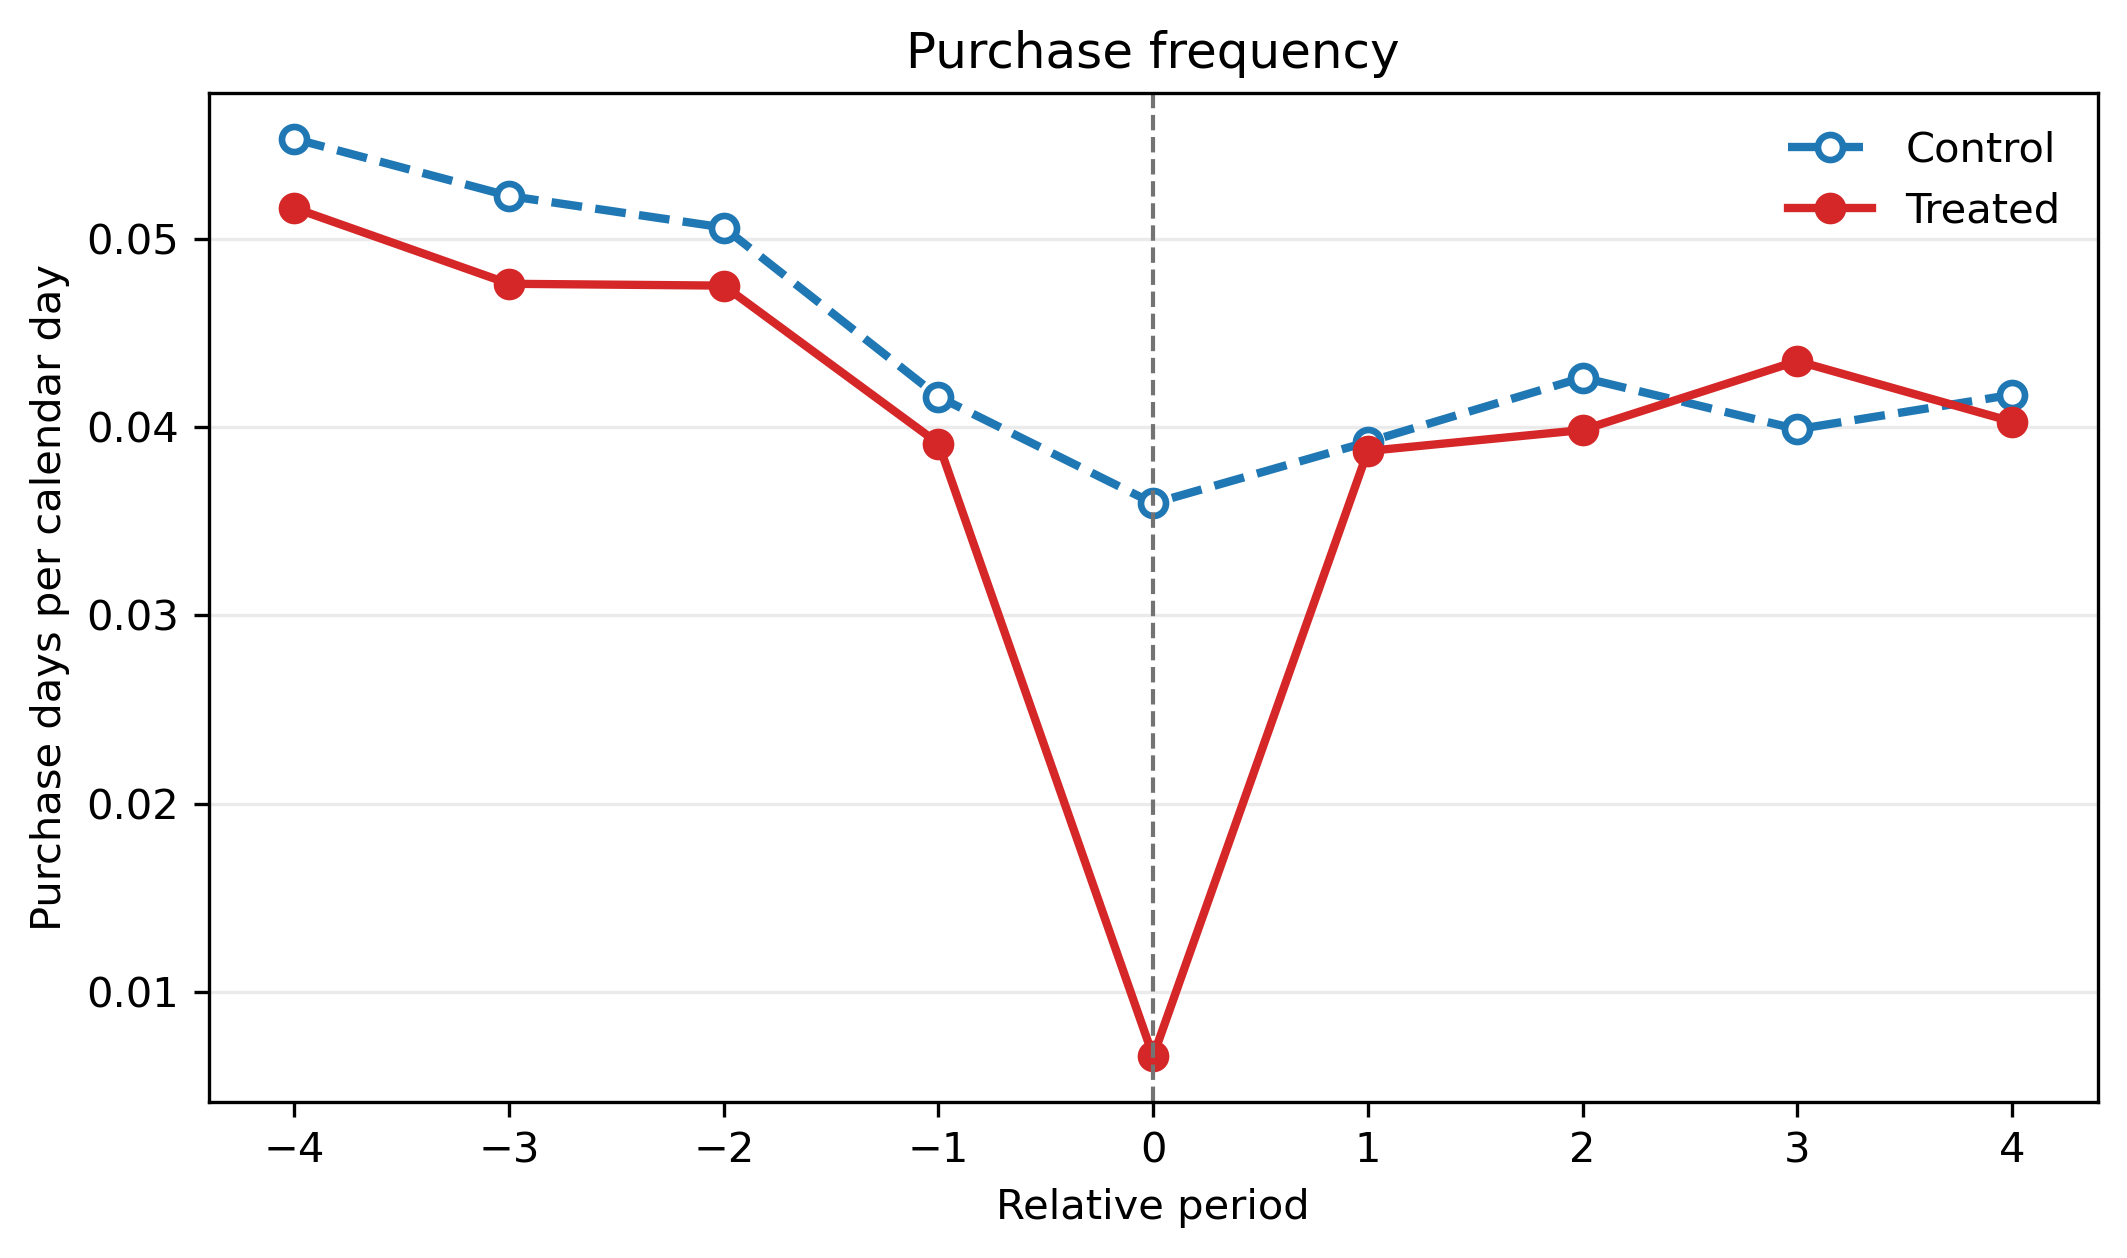
\includegraphics[width=0.78\textwidth]{figures/closure_shock_purchase_frequency.png}
	\caption{Store closures sharply reduce treated purchase frequency during the closure window}
	\label{fig:closure_shock_purchase_frequency}
\fnote{Notes: The figure plots consumer-weighted pooled means for the 18-closure analysis sample; each relative period contains 32,758 control and 7,390 treated consumer-events. Bars are 95\% confidence intervals. Relative period 0 is the closure window. Purchase frequency is the number of days divided by the number of calendar days in the event-length window.}
\end{figure}


\section{Empirical Strategy and Main Results}
\label{section:Empirical}

\subsection{Measuring Novelty-Seeking}
\label{section:Measuring Novelty-Seeking}

Let $i$ index consumers, $e$ closure events, $t$ relative periods, and let $L_e$ denote the duration in days of closure event $e$. For each event, relative periods $t=-4,\ldots,4$ have length $L_e$, with period 0 corresponding to the closure window. The estimation sample omits period 0 and compares four pre-closure windows with four post-reopening windows.

Our primary outcome measures exploration relative to the consumer's own purchase history. Let $\mathcal{J}_{iet}$ denote the set of distinct products that consumer $i$ purchases during event window $t$, and let $\mathcal{H}_{iet}^{-}$ denote the set of products the consumer purchased before that window. We define novelty-seeking as
\begin{equation}
\text{Y}^{N}_{iet}
=
\frac{\left|\mathcal{J}_{iet}\setminus\mathcal{H}_{iet}^{-}\right|}
{\left|\mathcal{J}_{iet}\right|}.
\label{eq:novelty_outcome}
\end{equation}
The set difference $\mathcal{J}_{iet}\setminus\mathcal{H}_{iet}^{-}$ contains the products purchased in the current window that do not appear in the consumer's prior purchase history, and $|\cdot|$ denotes the number of distinct products in a set. The outcome therefore ranges from zero to one. For example, if a consumer buys three distinct products in a window and one has never been purchased before, novelty-seeking equals $1/3$. A higher value means that a larger share of the consumer's current product set is unfamiliar based on her own observed history.

Novelty-seeking is defined only when the consumer purchases at least one product in the window, because otherwise the denominator in equation~\eqref{eq:novelty_outcome} is zero. The estimand concerns the \textit{composition of product choice conditional on purchasing}, rather than the probability of making a purchase. Accordingly, our estimates capture how purchase interruption changes the composition of realized product choices, and not its unconditional effect on the probability of exploring a novel product. Section~\ref{section:robustness_new_product} complements this consumer-specific measure with new-product-seeking, which instead classifies novelty according to whether a product has recently appeared in the chain.

\begin{figure}[!ht]
	\centering
	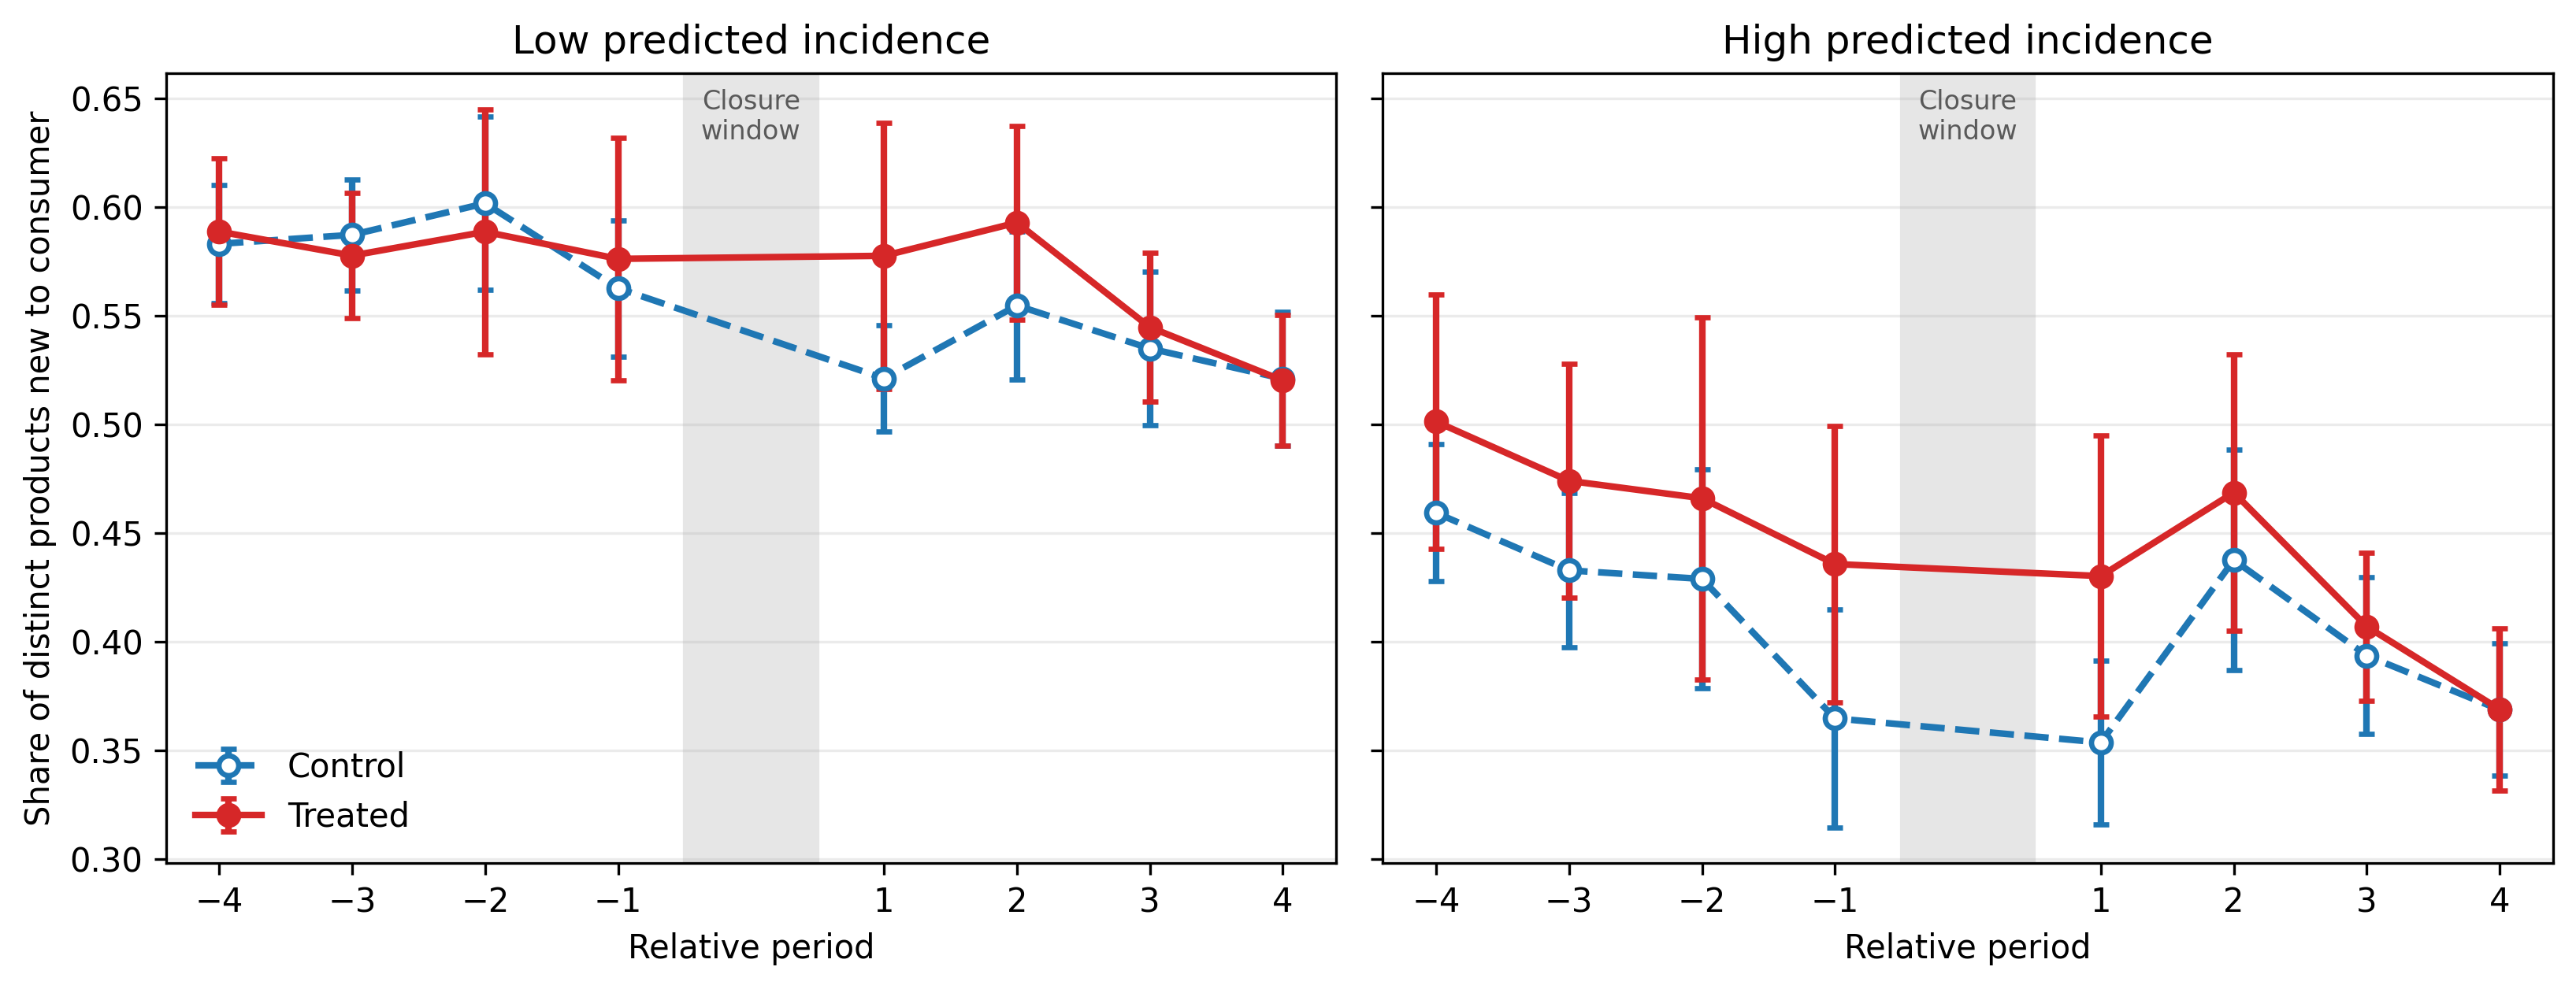
\includegraphics[width=0.96\textwidth]{figures/novelty_intention_paths.png}
	\caption{Raw novelty-seeking paths motivate the high-minus-low comparison}
	\label{fig:novelty_intention_paths}
\fnote{Notes: The figure plots consumer-weighted pooled means for the 18-closure analysis sample. Bars are 95\% confidence intervals. Across the eight plotted periods, observed-window counts range from 4,227 to 6,354 for control-low, 919 to 1,397 for treated-low, 4,918 to 7,469 for control-high and 1,171 to 1,714 for treated-high consumers. Relative period 0, the closure window, is omitted.}
\end{figure}

Figure~\ref{fig:novelty_intention_paths} plots the raw novelty-seeking paths for the four cells underlying the triple-differences design. In the low-predicted-intention group, treated and control means are close before the closure and the treated-control gap becomes more positive after reopening. In the high-predicted-intention group, the post-reopening change in the treated-control gap is much smaller. The empirical object of interest is precisely this difference between the two treated-control responses, which motivates the high-minus-low comparison estimated below.

Because novelty-seeking is observed only in purchasing windows, Figure~\ref{fig:purchase_probability_paths} plots the probability that a consumer makes at least one purchase in each relative period. This probability is also the probability that the consumer-event-period enters the novelty-seeking sample. Within each predicted-intention stratum, treated and control purchase-probability paths track closely around reopening. Thus, the product-choice result is not accompanied by a comparably large treated-control divergence in the extensive margin within either intention group. The absence of a large treated-control divergence in purchase probability reduces concerns that the novelty result is mechanically driven by differential sample entry, although it does not eliminate selection among consumers who purchase. We therefore retain a conditional-on-purchase interpretation throughout.

\begin{figure}[!ht]
	\centering
	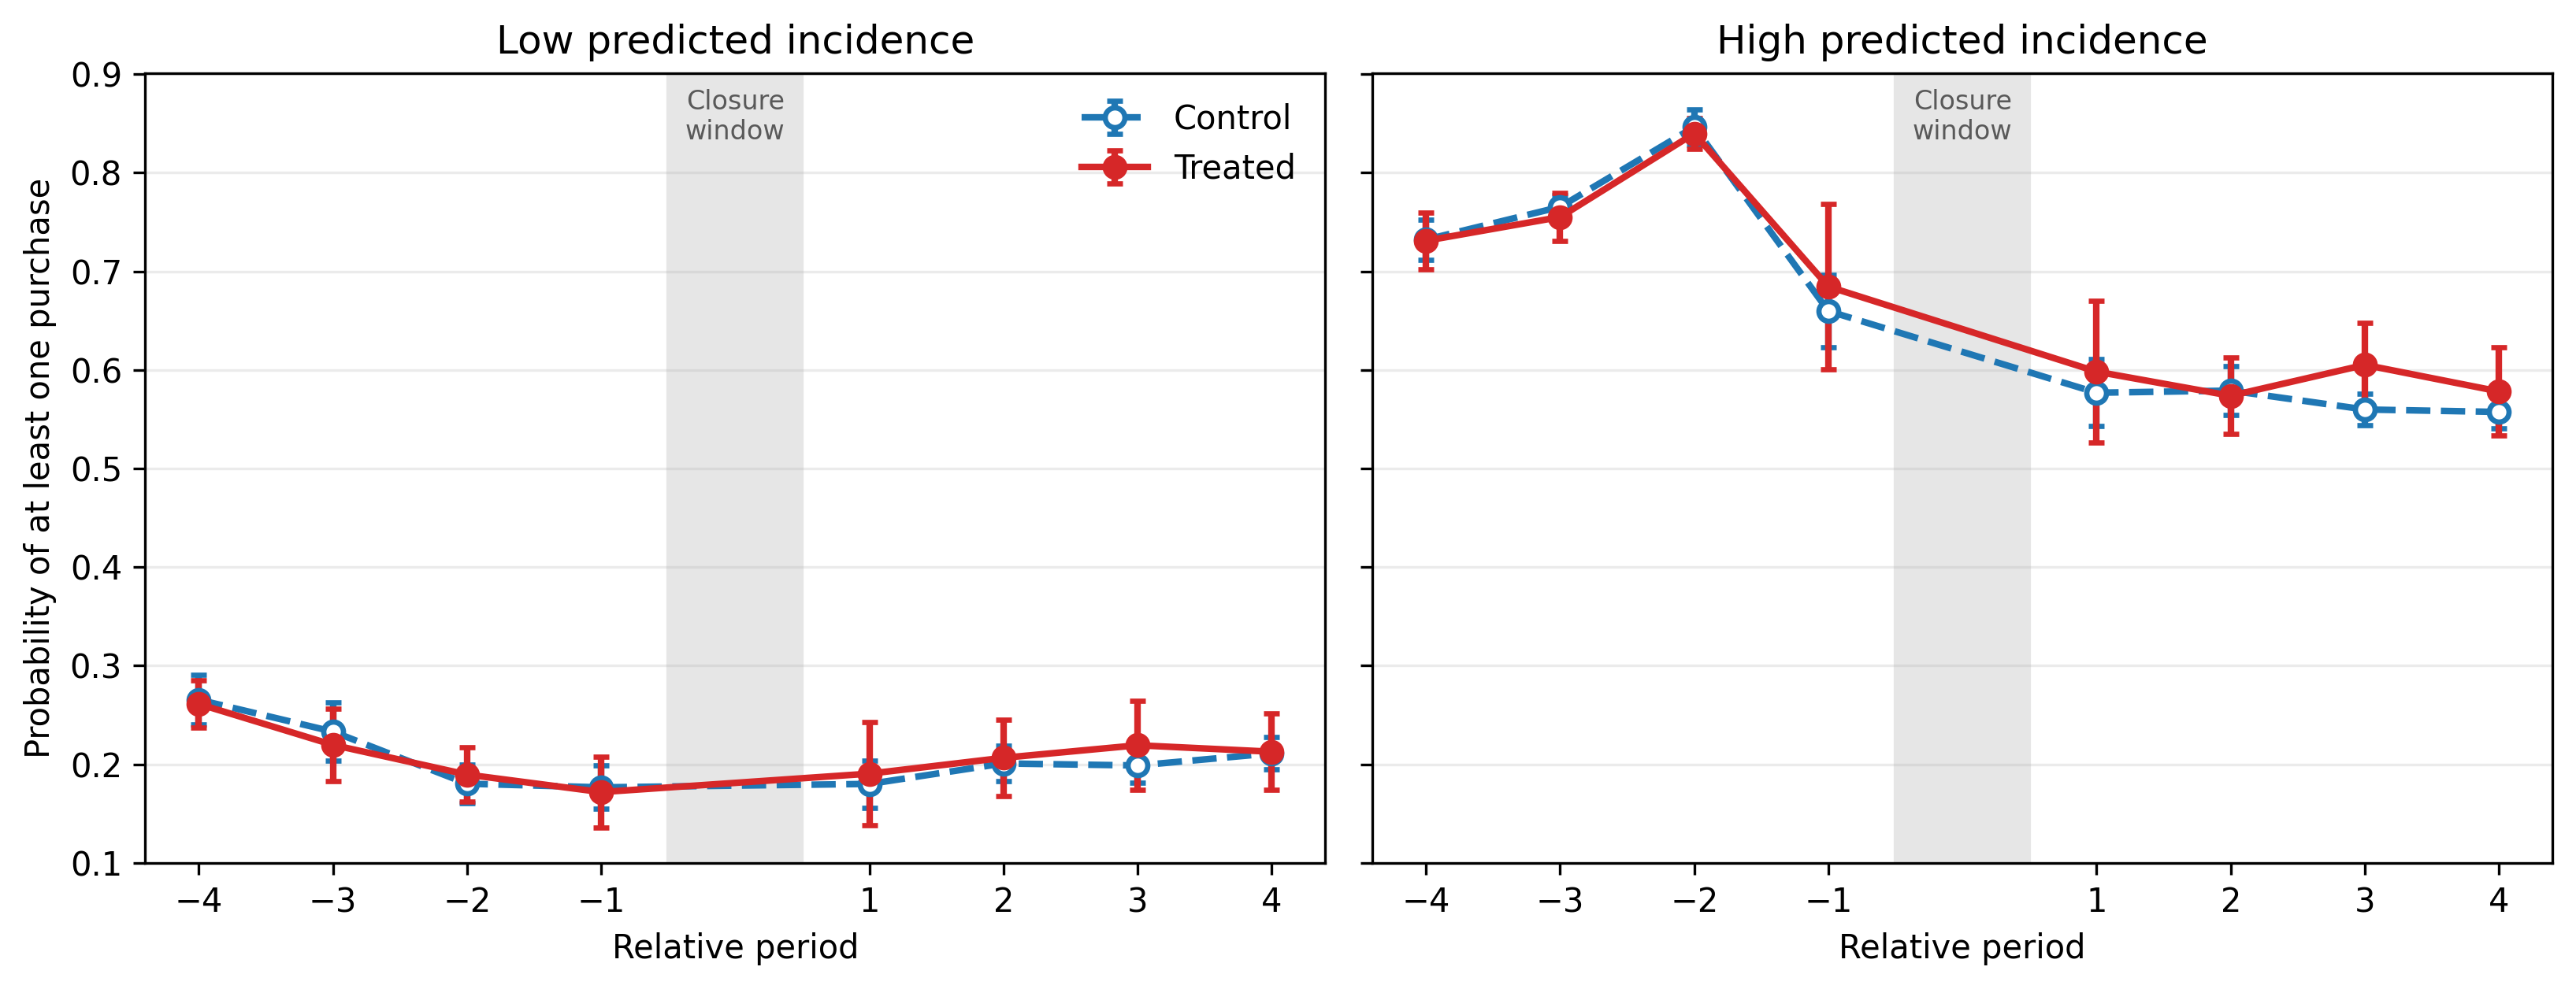
\includegraphics[width=0.96\textwidth]{figures/purchase_probability_paths.png}
	\caption{Purchase probability evolves similarly for treated and control consumers within predicted-intention groups}
	\label{fig:purchase_probability_paths}
\fnote{Notes: The figure plots the share of consumer-event-period observations containing at least one purchase. This is also the share of windows in which novelty-seeking is defined. Each relative period contains 23,934 control-low, 5,349 treated-low, 8,824 control-high and 2,041 treated-high consumer-events. Bars are 95\% confidence intervals. Means are consumer weighted. Relative period 0 is omitted to match the main regressions.}
\end{figure}

\subsection{Triple Difference-in-Differences}
\label{section:3.3}

To isolate the incremental response associated with interrupting a likely purchase, we compare (i) treated and control consumers, (ii) behavior before and after reopening, and (iii) consumers with high and low predicted purchase intention. It is useful to write the logic in two steps. For intention group $g\in\{L,H\}$, let $\Delta_g$ denote the treated-control difference-in-differences:
\begin{equation}
\Delta_g
=
\left(\overline{Y}_{T,g}^{Post}-\overline{Y}_{T,g}^{Pre}\right)
-
\left(\overline{Y}_{C,g}^{Post}-\overline{Y}_{C,g}^{Pre}\right).
\label{eq:group_did}
\end{equation}
$\Delta_L$ measures how novelty-seeking changes for treated low-intention consumers relative to comparable controls after reopening. Because these consumers were relatively unlikely to purchase during the closure, this contrast primarily captures consequences of closure exposure that do not require an intended purchase to have been blocked. $\Delta_H$ measures the analogous treated-control response among high-intention consumers, for whom the same closure is much more likely to interrupt a purchase. The triple difference is
\begin{equation}
DDD=\Delta_H-\Delta_L.
\label{eq:ddd_intuition}
\end{equation}
The third difference therefore removes the closure response observed among consumers for whom interruption was unlikely and leaves the incremental response associated with the closure being more likely to bind against an intended purchase. This logic follows the canonical triple-differences design \citep{Gruber1994} and is closely related to recent work using temporary disruptions to distinguish exposed consumers by the likelihood that a choice opportunity was displaced \citep{Levine2026}.

We implement this comparison in the pooled regression
\begin{equation}
Y^N_{iet}
=
\delta^B \cdot \text{Post}_{et} \times \text{Treated}_{ie}
+
\beta \cdot \text{Post}_{et} \times \text{High}_{ie}
+
\delta^D \cdot \text{Post}_{et} \times \text{Treated}_{ie} \times \text{High}_{ie}
+
\phi_{ie}+\omega_t+\gamma_m+\varepsilon_{iet},
\label{eq:main_ddd}
\end{equation}
where $Y^N_{iet}$ is novelty-seeking from equation~\eqref{eq:novelty_outcome}. $\text{Post}_{et}$ equals one in relative periods 1 through 4 and zero in relative periods $-4$ through $-1$. $\text{Treated}_{ie}$ equals one when consumer $i$ is assigned to the store that closes in event $e$, and $\text{High}_{ie}$ equals one when the ex-ante predicted purchase probability during the closure window is at least 0.5. Only the treated-high cell combines closure exposure with a high likelihood that an intended purchase was blocked.

The fixed effects serve distinct roles. Consumer-event fixed effects $\phi_{ie}$ absorb all characteristics that are constant within a consumer-event, including the levels of $\text{Treated}$, $\text{High}$, and their interaction. Relative-period fixed effects $\omega_t$ absorb common movement by event time, while calendar-month fixed effects $\gamma_m$ absorb calendar shocks shared by consumers observed in the same month, such as chain-wide changes in demand or product introductions. The remaining error is $\varepsilon_{iet}$. Because the access shock is shared by consumers within a closure event, standard errors are clustered by closure event.

The coefficients map directly to equations~\eqref{eq:group_did}--\eqref{eq:ddd_intuition}. For low-intention consumers, $\text{High}=0$, so the treated-control post response is $\delta^B=\Delta_L$. For high-intention consumers, the treated-control response is $\delta^B+\delta^D=\Delta_H$. Hence $\delta^D=\Delta_H-\Delta_L$ is the focal DDD. The coefficient $\beta$ captures a high-minus-low post shift that is common to treated and control consumers; it is not a closure effect. This decomposition is important for interpreting the estimates below: the causal object of interest is not the high-intention coefficient in isolation, but how the high-intention closure response differs from the low-intention closure response.

\subsection{Identification}
\label{section:3.3.1}

The interpretation of $\delta^D$ as the incremental effect of likely purchase interruption rests on two conditions. First, general consequences of closure exposure should affect high- and low-intention consumers similarly after taking the treated-control difference. A closure can change convenience, substitution opportunities, post-reopening promotions, or other aspects of the shopping environment even for consumers whose purchases were unlikely to be interrupted. These general consequences are captured by $\Delta_L$. The DDD subtracts them from $\Delta_H$, so $\delta^D$ isolates the interruption channel when these general closure effects do not themselves vary systematically with predicted purchase intention. A violation would arise, for example, if high-intention consumers responded differently from low-intention consumers to reopening promotions, substitution opportunities, or other consequences of the closure for reasons unrelated to whether a purchase was interrupted.

Second, absent the closure, the treated-control gap for high-intention consumers should have evolved like the treated-control gap for low-intention consumers. This is the parallel-triple-trends condition. Importantly, it concerns changes in the treated-control gaps rather than equality of pre-period levels. Consumer-event fixed effects absorb persistent level differences; identification requires that the \textit{difference between the two treated-control gaps} was not already trending before the closure.

We evaluate this condition using an event-study version of equation~\eqref{eq:main_ddd}. Relative period $-1$, the last pre-closure window, is the omitted reference. For each earlier pre-period $t\in\{-4,-3,-2\}$, we estimate the high-minus-low change in the treated-control gap relative to period $-1$, and then test whether the three pre-period DDD coefficients are jointly zero. For novelty-seeking, the three lead estimates range from 1.60 to 2.64 percentage points, every 95\% confidence interval includes zero, and the joint test yields $p=0.841$. The pre-period dynamics therefore provide no evidence that the high-minus-low treated-control gap was already moving before the focal closure. Appendix~\ref{app:identification_diagnostics} reports the full event-study coefficients and additional diagnostics.


\subsection{Main Results}
\label{section:Main Results}

Table~\ref{tab:main_results_decomposition} reports the group-specific closure responses and their difference. Reading the table from top to bottom is useful because the DDD is constructed from the first two rows. Among low-predicted-intention consumers, the treated-control post-reopening response is a 3.13-percentage-point increase in novelty-seeking (SE $=1.78$; $p=0.098$). Among high-predicted-intention consumers, the corresponding response is a 1.02-percentage-point decline (SE $=0.72$; $p=0.175$). The difference between these responses is $-4.15$ percentage points (SE $=1.84$; $p=0.038$), which is the focal estimate $\delta^D$.

\begin{table}[h!]
\centering
\caption{Purchase interruption narrows subsequent novelty-seeking}
\label{tab:main_results_decomposition}
\small
\begin{tabularx}{0.82\textwidth}{Xc}
\toprule
Effect & Novelty-seeking \\
\midrule
Low predicted purchase intention ($\delta^B$) & .0313* \\
 & (.0178) \\
 & [.0976] \\
High predicted purchase intention ($\delta^B+\delta^D$) & -.0102 \\
 & (.0072) \\
 & [.1745] \\
\addlinespace
\textbf{Incremental interruption effect: High minus low ($\delta^D$)} & \textbf{-.0415**} \\
 & \textbf{(.0184)} \\
 & \textbf{[.0380]} \\
\addlinespace
Pre-period outcome mean & .4978 \\
Observations & 99,644 \\
$R^2$ & .416 \\
Within $R^2$ & .001 \\
\bottomrule
\end{tabularx}
\vspace{1mm}
\fnote{Notes: Novelty-seeking is the share of distinct products purchased in a window that the consumer had not purchased before that window. The low- and high-intention rows report treated-control post contrasts within each predicted-intention group. The bold row is their difference, the focal triple-differences estimand. Standard errors, clustered by closure event (18 clusters), are in parentheses; p-values are in brackets. * $p<0.10$, ** $p<0.05$, *** $p<0.01$. All regressions include consumer-event, relative-period, and calendar-month fixed effects and omit the closure window.}
\end{table}

The positive 3.13-point response among low-intention consumers is informative about the general effect of closure exposure and about why the third difference is needed. Novelty is defined relative to each consumer's accumulated purchase history. During the closure, control consumers continue to purchase and can move products from the ``untried'' set into their familiar-product histories, while treated consumers have fewer opportunities to do so. Products introduced during the closure may likewise be tried by controls before treated consumers regain access. After reopening, a product can therefore remain classified as novel for a treated consumer even when it is already familiar to a comparable control consumer. These forces naturally push the low-intention treated-control contrast upward and represent consequences of the closure that do not require an intended purchase to have been interrupted. Importantly, Section~\ref{section:robustness_new_product} shows that the high-minus-low differential remains nearly identical when exploration is defined using recently introduced products rather than the consumer's accumulated purchase history.

The high-intention response is markedly different. For consumers whose purchase propensity during the closure was high, the treated-control contrast is 4.15 percentage points lower than the low-intention contrast. In other words, making the closure much more likely to bind against an intended purchase more than offsets the positive exploration response associated with closure exposure alone. The focal result is this \textit{difference between closure responses}, not the $-1.02$-point high-intention coefficient by itself. The DDD asks whether the high-intention response is different from the counterfactual closure response represented by the low-intention group, and the answer is a statistically significant $-4.15$-point shift.

The magnitude is economically meaningful. Relative to the pre-period mean novelty-seeking of 49.78\%, the 4.15-point DDD represents an 8.3\% reduction. Put differently, among purchasing windows, likely purchase interruption shifts the composition of subsequent purchases toward products already present in the consumer's history. Under the identifying conditions in Section~\ref{section:3.3.1}, this estimate supports Prediction 1: an intended but unrealized purchase narrows subsequent product exploration.

This interpretation also clarifies what the DDD contributes beyond a standard closure comparison. An average treated-control estimate would combine consumers for whom the closure merely changed access with consumers for whom it likely blocked an active purchase. The high-minus-low comparison separates these two components and reveals that the behavioral response associated with likely interruption runs in the opposite direction from the general closure-exposure response. Section~\ref{section:Mechanisms} next tests whether the cross-consumer pattern follows the heterogeneity predicted by familiar-choice salience and examines two concrete alternative explanations. Section~\ref{section:Robustness Checks} asks whether the same result appears when exploration is defined by adoption of products newly introduced by the firm.


\section{Evidence on Behavior Mechanism and Alternative Explanations}
\label{section:Mechanisms}

Prediction 2 provides a mechanism-linked test of familiar-choice salience. If an interrupted purchase reactivates an established consumption path, the reduction in exploration should be strongest among consumers whose prior choices are already more concentrated on familiar products. We test this implication using baseline novelty-seeking measured well before the focal closure. This test does not directly observe counterfactual thinking or goal persistence; rather, it examines whether the cross-consumer pattern follows a distinctive heterogeneity prediction implied by the proposed mechanism.

\subsection{Heterogeneity by Baseline Novelty-Seeking}
\label{section:Heterogeneity}

For each consumer-event, we calculate novelty-seeking separately in relative periods $-8$ through $-1$ and then average across periods in which the consumer purchases. Each of these periods has the same length as the associated closure event. Let $O_{ie}$ denote the number of distinct orders consumer $i$ places over these eight baseline windows. We require $O_{ie}\geq5$ so that the baseline measure is based on an established purchase history rather than one or two isolated transactions. The raw baseline novelty measure ranges from zero, when all purchased products are familiar, to one, when all distinct products purchased in each purchasing window are new relative to the consumer's earlier history.

The resulting sample contains 18,525 eligible consumer-events. Baseline novelty varies broadly: the mean is 0.508, the standard deviation is 0.269, the median is 0.500, and the 10th and 90th percentiles are 0.167 and 0.889. Figure~\ref{fig:baseline_novelty_distribution} shows that the heterogeneity test therefore uses variation across a wide range of exploratory behavior rather than a narrow split around a single cutoff.

\begin{figure}[!ht]
\centering
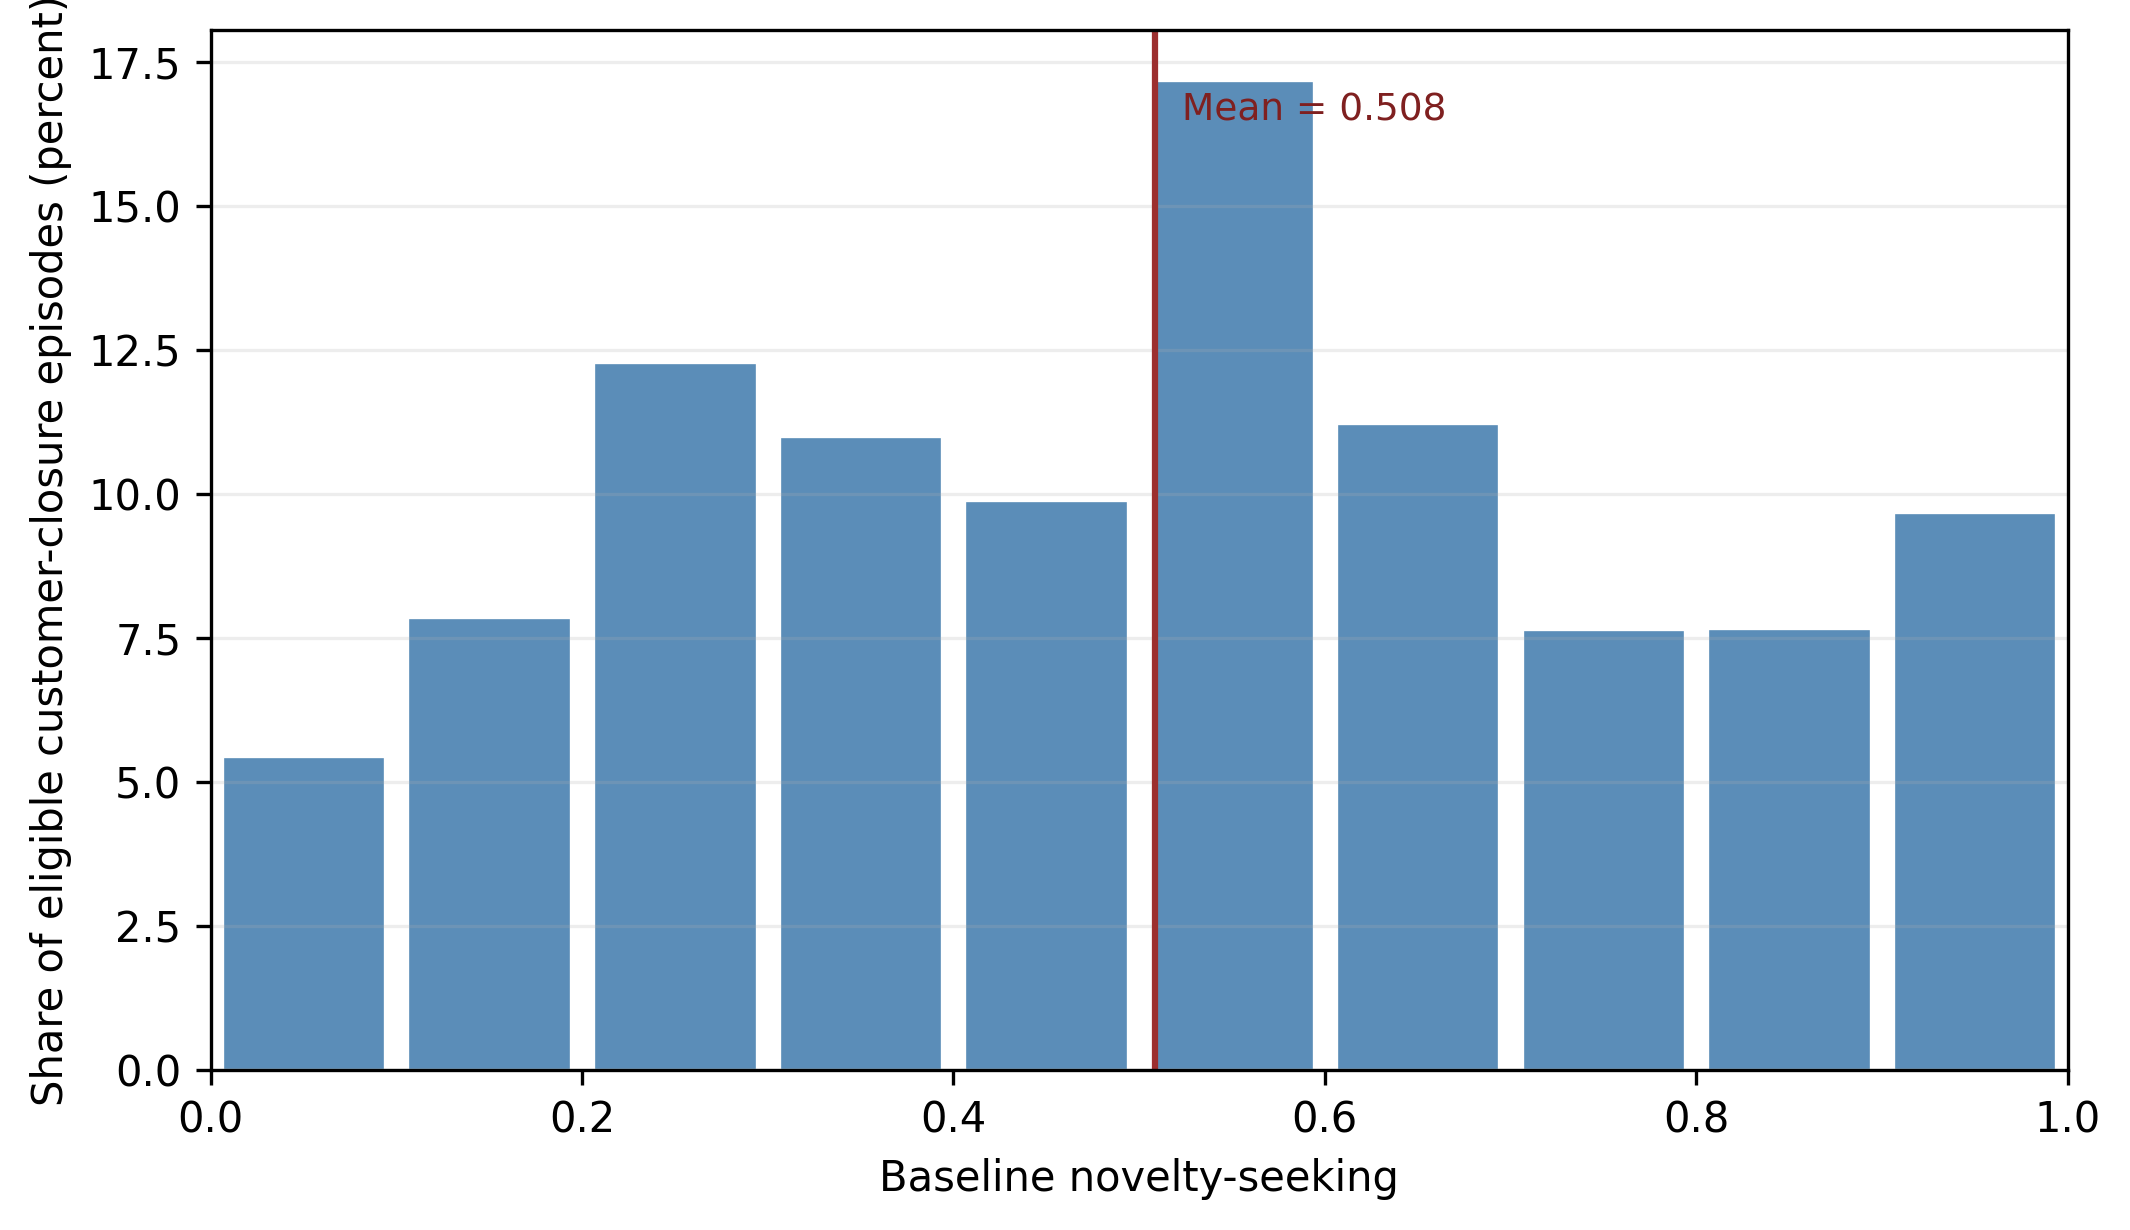
\includegraphics[width=0.78\textwidth]{figures/baseline_novelty_distribution.png}
\caption{Distribution of baseline novelty-seeking}
\label{fig:baseline_novelty_distribution}
\fnote{Notes: The figure shows ten equal-width bins of the raw consumer-level baseline novelty measure. The measure is the mean of within-period novelty-seeking over purchasing periods from relative period $-8$ through $-1$. Eligible consumers have at least five orders across these eight closure-length periods. The last bin includes one. The vertical line marks the sample mean. The sample contains 18,525 eligible consumer-events.}
\end{figure}

An important measurement feature is that baseline novelty is related to the amount of purchase history available. As consumers accumulate orders, more products enter their familiar set, so the same underlying willingness to explore can generate a lower measured novelty share when the observed history is longer. In the data, the correlation between baseline novelty and $\log(1+O_{ie})$ is $-0.329$. Mean baseline novelty is 0.620 among consumers with exactly five baseline orders and 0.365 among consumers with at least 20. We therefore want the heterogeneity coefficient to capture differences in exploratory orientation rather than differences in how much purchase history was available to construct that orientation.

To do so, let $N_{ie}$ denote standardized baseline novelty-seeking and define
\[
Q_{ie}
=
\frac{\log(1+O_{ie})-\overline{\log(1+O)}}
{\operatorname{SD}[\log(1+O)]},
\]
the standardized log number of baseline orders. Both $N_{ie}$ and $Q_{ie}$ have mean zero and unit standard deviation in the heterogeneity sample. Retaining the Post, Treated, and High definitions from equation~\eqref{eq:main_ddd}, we estimate
\begin{align}
Y^N_{iet}
={}& \delta^B(\text{Post}\times\text{Treated})
+\beta(\text{Post}\times\text{High})
+\delta^D(\text{Post}\times\text{Treated}\times\text{High}) \notag\\
&+\eta_0(\text{Post}\times N_{ie})
+\eta_T(\text{Post}\times\text{Treated}\times N_{ie})
+\eta_H(\text{Post}\times\text{High}\times N_{ie}) \notag\\
&+\theta^D(\text{Post}\times\text{Treated}\times\text{High}\times N_{ie}) \notag\\
&+\text{Post}\times Q_{ie}
\left(\kappa_0+\kappa_T\text{Treated}+\kappa_H\text{High}
+\kappa_D\text{Treated}\times\text{High}\right) \notag\\
&+\phi_{ie}+\omega_t+\gamma_m+\varepsilon_{iet}.
\label{eq:baseline_novelty_heterogeneity}
\end{align}

The first line reproduces the main DDD within the heterogeneity sample. The next two lines allow the post-period novelty response to vary with baseline novelty in every DDD cell. Specifically, $\eta_0$ is the post-period gradient with respect to baseline novelty for control, low-intention consumers; $\eta_T$ is the additional gradient for treated consumers within the low-intention group; $\eta_H$ is the additional gradient for high-intention consumers within the control group; and $\theta^D$ is the additional gradient for the treated-high cell beyond all lower-order components. Equivalently, $\theta^D$ tells us how the high-minus-low DDD changes when baseline novelty rises by one standard deviation.

The $Q_{ie}$ terms provide the analogous complete interaction hierarchy for the amount of baseline purchase history. $\kappa_0$ allows the post response to vary with baseline order history in the control-low cell; $\kappa_T$ and $\kappa_H$ allow that gradient to differ for treated and high-intention consumers; and $\kappa_D$ allows the DDD itself to vary with baseline orders. Because $N_{ie}$, $Q_{ie}$, treatment status, and predicted-intention status are time invariant within a consumer-event, their levels are absorbed by $\phi_{ie}$; only their interactions with Post are estimable. This complete hierarchy is important because it lets $\theta^D$ capture heterogeneity associated with baseline novelty \textit{holding the amount of baseline purchase history fixed}. Since $N_{ie}$ and $Q_{ie}$ are standardized, $\delta^D$ in this specification is the DDD evaluated at the mean baseline novelty and mean baseline order history of the heterogeneity sample. Prediction 2 implies $\theta^D>0$: as consumers become more exploratory, the negative interruption effect should attenuate.

\begin{table}[!ht]
\centering
\caption{Baseline novelty-seeking attenuates the interruption effect}
\label{tab:baseline_novelty_heterogeneity}
\small
\begin{tabularx}{0.82\textwidth}{Xc}
\toprule
 & Preferred specification \\
\midrule
DDD at mean baseline novelty and order history ($\delta^D$) & $-1.30$ \\
 & (2.00) \\
Change in DDD per SD of baseline novelty ($\theta^D$) & \textbf{2.94**} \\
 & (1.47) \\
One-sided $p$-value for $\theta^D>0$ & \textbf{.0312} \\
Joint pretrend $p$-value for $\theta^D$ & .5611 \\
Observations & 79,578 \\
Closure-event clusters & 18 \\
Consumer-event, relative-period, and calendar-month fixed effects & Yes \\
Post-by-baseline-order interaction hierarchy & Yes \\
\bottomrule
\end{tabularx}
\vspace{1mm}
\fnote{Notes: Estimates and standard errors are in percentage points. Baseline novelty-seeking is the consumer-level mean novelty over relative periods $-8$ through $-1$ and is standardized over eligible consumers. The specification also includes a complete Post-by-baseline-order interaction hierarchy using standardized $\log(1+\text{baseline orders})$, so $\theta^D$ captures how the interruption-related DDD changes with baseline novelty holding the amount of baseline purchase history fixed. Standard errors use CRV1 clustering by the 18 closure events.}
\end{table}

Table~\ref{tab:baseline_novelty_heterogeneity} reports the preferred specification. The focal estimate is $\theta^D=2.94$ percentage points (SE $=1.47$; one-sided $p=0.031$). Because a larger $\theta^D$ makes a negative DDD less negative, the sign is exactly the one predicted by familiar-choice salience: a one-standard-deviation increase in baseline novelty attenuates the interruption-related reduction in exploration by 2.94 points. The one-sided test corresponds to the directional Prediction 2, which specifically predicts $\theta^D>0$.

The size of the gradient is substantial relative to the headline effect. One standard deviation of raw baseline novelty is 0.269, so moving from one standard deviation below the mean to one standard deviation above the mean changes the fitted DDD by $2\times2.94=5.88$ percentage points. Holding baseline order history at its mean, the fitted DDD is approximately $-4.24$ points at a raw baseline novelty of 0.240 and $+1.63$ points at a raw baseline novelty of 0.777. These fitted values are illustrations of the estimated linear gradient rather than separately estimated subgroup effects, but they show where the aggregate result is concentrated: the familiar-choice response is strongest among consumers whose prior purchase histories reveal relatively little exploration and attenuates as consumers become more exploratory. The positive fitted value at high baseline novelty should therefore not be interpreted as evidence that interruption increases exploration for highly exploratory consumers; Prediction 2 concerns attenuation of the negative response, rather than a sign reversal.

The $-1.30$-point $\delta^D$ in Table~\ref{tab:baseline_novelty_heterogeneity} should not be read as a replacement for the $-4.15$-point main estimate. The heterogeneity regression uses a smaller sample restricted to consumers with at least five baseline orders, adds the full novelty and order-history interaction hierarchies, and evaluates $\delta^D$ at mean baseline novelty and mean order history. Its purpose is to identify the \textit{slope} $\theta^D$, not to re-estimate the unconditional headline DDD. Consistent with the interpretation of this slope, the heterogeneity event study shows no differential pretrend in $\theta^D$ ($p=0.561$). Appendix~\ref{app:baseline_novelty_dynamics} reports the dynamic estimates.

\subsection{Alternative Explanations}
\label{section:alternative_explanations}

We next examine two exposure-based explanations that could generate lower post-reopening exploration without the familiar-choice channel: differential exposure to new-product marketing and differential access to novel products after reopening. Each explanation requires a specific observable pattern in the data, allowing us to evaluate whether it can account for the sign and magnitude of the novelty DDD.

\subsubsection{New-Product Notifications}
\label{section:alternative_new_product_notifications}

The digital app sends push notifications to consumers based on their purchase histories, including campaigns that specifically promote newly introduced products. Consumers typically enter a ``dormant'' stage after 30 days without a purchase, and the firm's history-based notification algorithm determines subsequent messaging. This creates a plausible alternative explanation because the same purchase histories that predict intention can also affect notification exposure. If treated high-intention consumers systematically received fewer new-product messages after the closure, their lower exploration could reflect lower marketing exposure rather than a shift toward familiar choices.

To evaluate this channel, we count unique new-product campaigns received per consumer-day and estimate the same treated-control, high-minus-low comparison used for the main outcome. The sign required by the alternative explanation is negative: relative to the corresponding controls, treated high-intention consumers would need to receive fewer new-product campaigns than treated low-intention consumers. Instead, the estimated contrast is positive. During the closure, the relative high-minus-low exposure change is $+0.0041$ campaigns per consumer-day (95\% CI: $0.0019$ to $0.0064$; restricted wild-cluster $p=0.003$). After reopening, it remains positive at $+0.0017$ campaigns per day (95\% CI: $0.0001$ to $0.0032$; $p=0.047$), and the event-study leads do not reject a common pretrend ($p=0.500$).

The direction is informative. Treated high-intention consumers are targeted with \textit{more}, not fewer, new-product campaigns relative to the DDD comparison group. Although the records do not reveal whether consumers viewed these messages, the observed targeting differential runs in the opposite direction from that required by the notification-based explanation. If new-product notifications increase awareness or trial, this differential exposure would tend to raise their exploration and therefore work against the negative novelty DDD. The notification channel consequently cannot account for the observed reduction in novelty-seeking. Appendix~\ref{app:new_product_notifications} reports the campaign construction, alternative exposure measures, and complete estimates.

\subsubsection{Reopening Assortments}
\label{section:alternative_assortment}

A second explanation is that high- and low-intention consumers encounter different opportunities to choose novel products after reopening. This can occur if the store assortment changes over time and the two groups return at different times. We therefore separate the argument into two steps: whether realized assortments evolve after reopening, and whether the groups' actual return timing translates that evolution into meaningfully different exposure to products that are novel for each consumer.

We first characterize realized assortment at treated stores over four fixed seven-day periods after reopening. We use three complementary measures. \textit{Core-product coverage} is the share of regularly sold pre-closure products that continue to appear in a given week. \textit{Products per 50 baskets} measures the number of distinct products sold in standardized samples of 50 consumer-day baskets, which removes the mechanical effect of different transaction volumes. \textit{Pre-menu overlap} measures the similarity between products sold in a post-reopening week and the store's pre-closure product set. Core-product coverage does not change significantly across the four weeks ($p=0.382$ jointly), but standardized product breadth and pre-menu overlap do evolve ($p=0.011$ and $p=0.018$ jointly). Thus, assortment evolution is meaningful enough that return timing is worth evaluating directly rather than assuming that all returners face the same menu environment.

High-intention consumers do return earlier. Among treated consumers who return to the focal store within 28 days, high-intention consumers return 2.87 days earlier on average (SE $=0.29$); 53.6\% return in week 1 compared with 36.9\% of low-intention returners. To translate this timing difference into consumer-specific opportunity, we construct, for every returner and each possible return week, a leave-one-consumer-out realized product set. Excluding the focal consumer prevents her own purchase from mechanically affecting the measured assortment. We then calculate the share and count of products in that set that the consumer had never purchased by reopening. Finally, we subtract each consumer's own four-week average opportunity from the opportunity in the week in which she actually returns. This isolates the component of novel-product exposure generated by return timing rather than stable differences across consumers.

The timing-induced difference is much smaller than the main behavioral effect. The high-minus-low difference in the novel-product share is $-0.10$ percentage points (SE $=0.06$; 95\% CI: $-0.22$ to $+0.02$), about one-fortieth of the $-4.15$-percentage-point novelty DDD. The corresponding difference in the number of novel products is $-0.28$ products (SE $=0.38$; 95\% CI: $-1.09$ to $+0.54$). The store assortment does evolve and the groups do return at different times, but the combination of these two facts produces very little differential exposure to personally novel products.Within the realized transaction environment we observe, the assortment-timing channel is quantitatively too small to account for the magnitude of the main novelty-seeking result. Appendix~\ref{app:reopening_assortment} reports the weekly assortment paths, construction details, and matched-store comparisons.


\section{Robustness Checks}
\label{section:Robustness Checks}

We conduct four sets of robustness analyses around the main novelty-seeking result. First, the main specification classifies consumers into high- and low-predicted-intention groups using a cutoff of 0.5. We replace this binary classification with the continuous predicted purchase probability to examine whether the result depends on the particular threshold. Second, our main novelty measure defines a product as novel when the consumer has not purchased it before. We use an alternative measure based on products that have recently appeared in the chain to examine whether purchase interruption also affects new-product adoption. Third, because a substantial share of purchases in our setting involves coffee, we re-estimate the novelty-seeking specification using only non-coffee products. Finally, we account for differences in the local competitive environment surrounding consumers' preferred stores and for broader local post-reopening shocks.

\subsection{Continuous Predicted Purchase Probability}
\label{section:robustness_continuous_score}

Our main specification converts the predicted purchase probability into a binary indicator, $\text{High}_{ie}$, using a cutoff of 0.5. Although this classification gives the DDD a transparent interpretation, consumers whose predicted probabilities are 0.49 and 0.51 are assigned to different groups despite having similar predicted purchase intentions. We therefore examine whether the main result also appears when we use the full variation in predicted purchase probability.

Let $s_{ie}\in[0,1]$ denote the predicted probability that consumer $i$ would make at least one purchase during the closure window associated with event $e$, and let
\[
\widetilde{s}_{ie}=s_{ie}-\bar{s}
\]
denote the score centered at its estimation-sample mean. Replacing $\text{High}_{ie}$ in equation~\eqref{eq:main_ddd} with $\widetilde{s}_{ie}$ gives
\begin{equation}
Y^N_{iet}
=
\delta_0^B
\left(
\text{Post}_{et}\times\text{Treated}_{ie}
\right)
+
\beta^S
\left(
\text{Post}_{et}\times\widetilde{s}_{ie}
\right)
+
\delta^S
\left(
\text{Post}_{et}\times\text{Treated}_{ie}\times\widetilde{s}_{ie}
\right)
+
\phi_{ie}+\omega_t+\gamma_m+\varepsilon_{iet}.
\label{eq:continuous_score_robustness}
\end{equation}
Because the score is centered, $\delta_0^B$ measures the treated-control post-reopening response for a consumer with the average predicted purchase probability. The coefficient $\beta^S$ captures how the post-period outcome varies with predicted purchase intention in a way common to treated and control consumers. The coefficient of interest is $\delta^S$: it measures how the treated-control post-reopening response changes as the predicted probability that the closure interrupted a purchase increases. A negative $\delta^S$ therefore corresponds directly to the prediction that consumers whose purchases were more likely to have been interrupted subsequently exhibit a larger reduction in novelty-seeking.

Using novelty-seeking as the dependent variable, we estimate $\delta^S=-0.0452$ (SE $=0.0276$; $p=0.120$). Since the predicted-intention score ranges from zero to one, this coefficient implies that a 10-percentage-point increase in predicted purchase intention is associated with a 0.45-percentage-point more negative treated-control post-reopening response in novelty-seeking. The continuous specification therefore preserves the negative relationship between predicted purchase intention and the treated-control post-reopening response found in the binary specification, although the interaction is not statistically distinguishable from zero. Although the continuous estimate is less precisely estimated under closure-level clustering, its sign and economic gradient show that the main result is not generated mechanically by the 0.5 classification threshold. Appendix Table~\ref{tab:appendix_score_main_results} reports the complete specification and corresponding diagnostics.

\subsection{Alternative Outcome Definition: New-Product-Seeking}
\label{section:robustness_new_product}

Our main novelty-seeking measure focuses on whether consumers depart from their own familiar purchase histories. An alternative perspective, especially relevant for firms introducing new products, is whether consumers adopt products that have recently appeared in the marketplace. The two measures capture related but distinct forms of exploration. A product may be new to a particular consumer even if it has been sold by the firm for a long time, whereas a recently introduced product represents an innovation from the firm's perspective.

Let $F_j$ denote the first date on which product $j$ appears in the chain's transaction records, and let $\mathcal{W}_{et}$ and $\mathcal{W}_{e,t-1}$ denote the current and immediately preceding event windows. We define new-product-seeking as
\begin{equation}
Y^{NP}_{iet}
=
\frac{
\left|
\left\{
j\in\mathcal{J}_{iet}:
F_j\in\mathcal{W}_{e,t-1}\cup\mathcal{W}_{et}
\right\}
\right|
}{
|\mathcal{J}_{iet}|
}.
\label{eq:new_product_maintext}
\end{equation}
Thus, $Y^{NP}_{iet}$ is the share of distinct products purchased in the current window whose first observed chain sale occurs in either the current or immediately preceding event window. Like the main novelty measure, it is defined conditional on the consumer making a purchase. The first observed sale serves as our empirical measure of when a product newly appears in the chain.

We first apply the binary DDD specification in equation~\eqref{eq:main_ddd}. Among low-predicted-intention consumers, the treated-control post-reopening response in new-product-seeking is $+0.80$ percentage points (SE $=1.13$; $p=0.487$). Among high-predicted-intention consumers, the corresponding response is $-3.37$ percentage points (SE $=1.45$; $p=0.033$). Their difference is $-4.17$ percentage points (SE $=0.89$; $p<0.001$), equivalent to 28.6\% of the 14.56\% pre-period mean. The high-minus-low pretrend test does not reject parallel trends ($p=0.114$).

This result strengthens the interpretation of the main finding in two ways. First, the $-4.17$-point DDD is almost identical in absolute magnitude to the $-4.15$-point estimate obtained when novelty is defined relative to the consumer's own history. Second, the high-intention treated consumers themselves exhibit a 3.37-point decline in adoption of recently appearing products. Thus, the reduction in exploration is not driven solely by the history-dependent construction of the main novelty measure; likely purchase interruption is also associated with a lower propensity to adopt products that have recently entered the market.

We further apply the continuous-score specification in equation~\eqref{eq:continuous_score_robustness}, replacing the dependent variable with $Y^{NP}_{iet}$. The treatment-by-score coefficient is $-4.86$ percentage points (SE $=1.56$; $p=0.006$) for a one-unit increase in predicted purchase probability. Equivalently, increasing predicted purchase intention by 10 percentage points makes the fitted treated-control post-reopening response in new-product-seeking 0.49 percentage points more negative. The corresponding continuous-score pretrend test does not reject ($p=0.377$). The binary and continuous specifications therefore lead to the same conclusion: the more likely the closure was to interrupt a purchase, the less consumers subsequently adopt recently appearing products. Appendix~\ref{app:new_product_seeking} reports the complete coefficient decompositions and diagnostics.

\subsection{Effect on Non-Coffee Products}
\label{section:robustness_noncoffee}

We next examine whether the negative novelty-seeking response is specific to coffee products. Coffee consumption can be strongly habitual, and the caffeine content of many products may further reinforce repeated consumption. If the main result were driven entirely by features specific to coffee, its implications for novelty-seeking in other product categories would be more limited. We therefore re-estimate the same binary DDD specification using only non-coffee products. Because these restrictions substantially reduce the number of qualifying purchasing windows, we view this exercise as a product-scope sensitivity analysis rather than an independent causal test.

Based on the commodity-description fields, we construct three increasingly restrictive product scopes. The broadest definition includes all non-coffee products, including non-coffee beverages, food, and other items. The second retains only non-coffee consumables---beverages and food---and the third retains only non-coffee beverages. Within each scope, novelty-seeking is defined in the same way as the main outcome: the share of distinct qualifying products purchased in a window that the consumer had not purchased previously. Consequently, the outcome is observed only for windows in which the consumer makes at least one purchase from the corresponding product group.

Across all three product scopes, the estimated DDD remains negative. For all non-coffee products, the estimate is $-4.13$ percentage points (SE $=3.40$; restricted wild-cluster $p=0.225$), remarkably close in magnitude to the $-4.15$-point main result. Restricting the outcome to non-coffee consumables produces an estimate of $-4.11$ percentage points (SE $=3.39$; restricted wild-cluster $p=0.230$). Restricting the sample further to non-coffee beverages produces a larger estimate of $-6.26$ percentage points (SE $=4.12$; restricted wild-cluster $p=0.119$). Thus, the negative product-choice pattern is present not only in coffee choices but also when coffee products are removed entirely.

The narrower product definitions substantially reduce the number of purchasing windows on which novelty can be measured: the corresponding estimation samples contain 30,444 observations for all non-coffee products, 30,418 for non-coffee consumables, and 21,433 for non-coffee beverages, compared with 99,644 observations for the main novelty outcome. We therefore use these analyses primarily to examine whether the direction and economic magnitude of the result are specific to coffee, rather than treating them as separate headline estimates.

The accompanying diagnostics also differ across product scopes. For all non-coffee products and non-coffee consumables, the joint high-minus-low pretrend tests reject equality of the leads ($p=0.006$ in both cases). For non-coffee beverages, the novelty-seeking pretrend test does not reject ($p=0.226$), while the probability of making a qualifying purchase declines differentially for high-intention treated consumers after reopening: the corresponding DDD is $-2.24$ percentage points (SE $=0.90$; $p=0.023$). Because novelty-seeking is observed only when a qualifying purchase occurs, this extensive-margin response can change the set of consumers entering the beverage-specific novelty regression. We therefore interpret the non-coffee exercise as evidence on the scope of the behavioral pattern: the negative relationship is not unique to coffee products, while the main all-product specification remains the preferred basis for causal inference. Appendix~\ref{app:noncoffee_novelty} reports the complete estimates, sample-entry analyses, and event-study diagnostics.

\subsection{Accounting for Local Competition}
\label{section:robustness_competing_brands}

Local competition may affect consumers' product choices after reopening and could therefore contribute to the post-reopening treated-control differences in novelty-seeking. To account for this possibility, we supplement the transaction data with store-address data that report the number of potentially competing establishments located within 500 and 1,500 meters of each store. We use the 500-meter count as our primary measure of local competition and assign it to each consumer-event through the consumer's preferred store in the pre-closure period. The 1,500-meter count provides an alternative measure using a broader geographic market. Our objective is not to identify local competition as a moderator of the interruption effect, but to assess whether differences in the observed competitive environment can account for the main negative DDD.

Because these competitor counts are time invariant, their levels are absorbed by the consumer-event fixed effects. We therefore allow local competition to affect changes after reopening by interacting it with the post-period indicator, treatment status, and predicted purchase intention. Let $\widetilde C_s$ denote the standardized competitor count associated with preferred store $s$. We augment equation~\eqref{eq:main_ddd} with
\begin{equation}
\text{Post}_{et}
\Big[
\kappa_C\widetilde C_s
+
\kappa_{TC}
\left(
\text{Treated}_{ie}\widetilde C_s
\right)
+
\kappa_{HC}
\left(
\text{High}_{ie}\widetilde C_s
\right)
+
\kappa_{THC}
\left(
\text{Treated}_{ie}\text{High}_{ie}\widetilde C_s
\right)
\Big].
\label{eq:local_competition_ddd}
\end{equation}
The original $\text{Post}\times\text{Treated}$, $\text{Post}\times\text{High}$, and $\text{Post}\times\text{Treated}\times\text{High}$ terms remain in the regression. Because $\widetilde C_s$ is standardized to have mean zero, the coefficient $\delta^D$ on the original triple interaction is the fitted novelty-seeking DDD at the average observed level of local competition. More generally, at a standardized competition level $c$, the fitted DDD is
\[
\delta^D+\kappa_{THC}c.
\]
The coefficient $\kappa_{THC}$ therefore describes how the fitted DDD varies with local competition, while the primary purpose of this specification is to examine whether accounting for the observed competitive environment changes the negative interruption effect.

The main result remains economically similar after introducing these interactions. Using the raw number of potentially competing establishments within 500 meters, the fitted DDD at the mean level of competition is $-3.33$ percentage points (95\% CI: $-6.35$ to $-0.31$), compared with $-4.15$ percentage points in the baseline specification. Using $\log(1+\text{competitor count})$ instead produces a fitted DDD of $-3.92$ percentage points (95\% CI: $-7.64$ to $-0.20$). Expanding the geographic radius to 1,500 meters yields estimates of $-4.04$ percentage points using the raw count and $-4.11$ percentage points using its logarithm. Thus, the negative interruption-related novelty response is similar across alternative measures of the local competitive environment.

We also evaluate the raw 500-meter specification at different levels of competition. At competitor counts of 2, 5, and 13---corresponding to the 25th percentile, median, and 75th percentile among the design stores---the fitted DDDs are $-5.03$, $-4.39$, and $-2.70$ percentage points, respectively. The estimated change in the DDD associated with a one-standard-deviation increase in local competition is $+3.00$ percentage points, with a 95\% confidence interval from $-5.15$ to $11.14$ points. We therefore do not use these estimates to make a separate claim about competition as a moderator; rather, the relevant robustness result is that the fitted interruption effect remains negative over a broad range of observed competitive environments.

Finally, the competitor counts cannot capture every local change that may occur around reopening. We therefore conduct an additional specification that includes preferred-store-by-event-by-post fixed effects. These fixed effects allow each preferred store within each closure event to have its own post-reopening shift and thereby absorb additive local changes---such as neighborhood demand conditions, local promotions, or other store-specific shocks---that are common to high- and low-predicted-intention consumers associated with that store. Identification of the DDD then comes from the differential post-reopening response between high- and low-intention consumers within the same preferred-store and closure-event environment. With these fixed effects, the novelty-seeking DDD is $-4.45$ percentage points (SE $=1.71$; 95\% CI: $-8.07$ to $-0.84$), again close to the $-4.15$-point headline estimate.

Taken together, these analyses show that the main novelty-seeking result is not explained by observed differences in local competition or by additive post-reopening shocks shared by consumers associated with the same preferred store. Appendix~\ref{app:robustness_competing_brands} reports the construction of the competition measures, alternative geographic definitions, fitted effects at different competition levels, and the corresponding event-study diagnostics.


\section{Conclusion}
\label{section:7}

This paper asks how consumers' willingness to explore changes when a purchase they likely intended to make is unexpectedly blocked. Using temporary store closures as exogenous changes in access and predicted purchase intention to distinguish likely interruption from general closure exposure, we find that likely purchase interruption reduces subsequent novelty-seeking by 4.15 percentage points, or 8.3\% of the pre-period mean. The result is nearly identical when exploration is measured by adoption of products newly introduced by the firm: the estimated DDD is $-4.17$ percentage points, or 28.6\% of that outcome's pre-period mean.

The decomposition of the main DDD is central to the interpretation. Low-intention consumers exhibit a positive closure-related novelty response, consistent with the fact that reduced purchasing during closure leaves more products untried in their observed histories. When the closure is much more likely to interrupt an intended purchase, however, the product-choice response shifts downward by 4.15 points. This high-minus-low difference reveals a behavioral consequence that an average closure effect would obscure: likely interruption pulls subsequent purchasing toward the familiar product set relative to the general product-choice response generated by closure exposure.

The cross-consumer pattern follows the mechanism-linked prediction of familiar-choice salience. Consumers with lower baseline novelty-seeking show the strongest interruption response; a one-standard-deviation increase in baseline novelty attenuates the DDD by 2.94 percentage points. Two concrete exposure-based explanations do not reproduce the pattern. Treated high-intention consumers receive more, rather than fewer, new-product notifications, and their earlier return timing generates only a 0.10-percentage-point reduction in exposure to personally novel assortments, far smaller than the headline effect. Together with the parallel pre-period dynamics and the new-product-seeking result, these findings support the interpretation that an intended but unrealized purchase can carry forward into subsequent product choice.

The managerial implication is that the value of product innovation depends partly on consumers' recent purchase experiences. After store closures, stockouts, app outages, delivery suspensions, or other temporary access constraints, recently interrupted consumers may be less receptive to unfamiliar offerings and more responsive to familiar choices. Firms can use this heterogeneity when timing and targeting new-product launches, designing personalized recommendations, and allocating promotional incentives. When targeting is flexible, familiar products may be more effective recommendations for consumers whose likely purchases were blocked, while early new-product promotion can be directed toward less-affected consumers. When rapid diffusion makes those interrupted consumers important targets, stronger trial incentives such as coupons or price promotions may be needed to offset their greater pull toward familiarity. Purchase interruption therefore shapes not only whether consumers can transact today, but also what they are willing to discover tomorrow.


\bibliographystyle{JMRstyle}
\bibliography{References}

%%%%-----------------------------Web Appendix-----------------------------------------%%%%
\newpage
\appendix

\setcounter{figure}{0}
\renewcommand{\thefigure}{W\arabic{figure}}

\setcounter{table}{0}
\renewcommand{\thetable}{W\arabic{table}}

\setcounter{footnote}{0}
\renewcommand{\thefootnote}{\alph{footnote}}

\clearpage
\section*{\centering Web Appendix}


\section{Data Construction and Measurement}
\label{app:data_construction}

This appendix records construction details that are needed to interpret the empirical design but are too mechanical for the main text. The unit of assignment is a consumer-event. A consumer enters the analysis through a closure event for which the consumer's pre-closure purchase history identifies a meaningful focal store; the outcomes then aggregate that consumer's purchases across the observed chain.

\subsection{Closure Registry and Consumer-Event Sample}
\label{app:closure_registry}

The raw data contain 7,312,498 orders, represented by 10,631,250 product-line records, from 779,744 consumers at 260 stores between June 1, 2020 and December 31, 2021. We aggregate these orders to a store-day panel and define a candidate closure as a consecutive spell in which a store records no transactions. This procedure identifies 101 zero-transaction spells.

We first remove 60 spells at stores located in universities or colleges. These spells occur during summer periods in which COVID-19 policies may have kept students away from campus. Because the data cover purchases made in this city, we do not observe whether students continued to buy from the chain elsewhere. A campus store with no local transactions may therefore reflect the temporary absence of its consumers rather than a supply disruption. Removing these spells avoids treating a seasonal loss of the local consumer population as a store closure and leaves 41 non-campus candidates.

We next exclude seven spells lasting 30 days or longer. The analysis is designed around short disruptions followed by a clearly observed reopening; longer spells are more likely to reflect seasonal shutdowns or persistent changes in store operations. They also produce much longer pre- and post-event windows, which are difficult to compare within the 19-month data period. Requiring closures to last strictly fewer than 30 days leaves 34 candidates.

The remaining events must provide enough support for the treated-control comparison. We require at least one treated and one control consumer and at least 50 consumers in each group. These restrictions remove events for which the DDD is undefined or rests on a very small group. We also require the control purchase rate during the closure to be at least twice the treated rate. This screen is intended to distinguish a localized access disruption from a broader contraction in demand that affects treated and control consumers alike. Together, the support and purchase-rate screens remove 12 events---eight for a low control purchase rate, two for insufficient group size and two for having no control consumers---leaving 22 closures. Because the purchase-rate screen uses behavior realized during the closure, the full-registry sensitivity analysis remains important.

The maintained headline sample excludes four additional events around the Lunar New Year period. Travel, holiday schedules and COVID-19-related mobility changes during this period can shift consumer traffic independently of a store closure, and these events have weaker treatment-control fit. This restriction leaves 18 closures lasting 10 to 29 days. It is not generated by a coded ex-ante rule, so we retain the 22-event full-registry analysis as a sensitivity check and report it below.

For each retained closure, treated consumers are those whose preferred pre-closure store is the store that closes. Control consumers are those whose preferred store is one of the matched stores that remains open. We process closures chronologically and, without replacement, match each closing store to the five eligible stores with the smallest absolute difference in setup date, a predetermined store characteristic. Candidate controls exclude all treated stores, previously selected controls, and university or college stores. We define the preferred store from pre-closure purchases and require at least five pre-closure purchase days and a preferred-store purchase share of at least 80\%. These restrictions ensure that the closing store was an economically meaningful source of access for treated consumers. The final sample contains 40,148 consumer-events: 7,390 treated and 32,758 controls. Of the treated consumers, 2,041, or 27.6\%, have high predicted purchase intention during the closure window.

\subsubsection{Sensitivity to the Closure Registry}

Table~\ref{tab:closure_registry_sensitivity} compares the full 22-event registry with the preferred 18-event registry using the same novelty measure and DDD specification. Retaining the four Lunar New Year events produces a DDD of $-3.86$ percentage points (SE $=1.67$; $p=0.031$), close to the $-4.15$-point estimate in the preferred registry. The displacement pretrend test does not reject in either sample ($p=0.707$ and $p=0.841$, respectively). Thus, the magnitude and inference are not driven by excluding these four events.

\begin{table}[!ht]
\centering
\caption{Novelty-seeking DDD across closure registries}
\label{tab:closure_registry_sensitivity}
\small
\begin{tabularx}{\textwidth}{Xrrrrrr}
\toprule
Closure registry & Events & DDD & SE & $p$-value & Observations & Pretrend $p$-value \\
\midrule
Full registry & 22 & $-3.86$ & 1.67 & .031 & 113,269 & .707 \\
Preferred registry & 18 & $-4.15$ & 1.84 & .038 & 99,644 & .841 \\
\bottomrule
\end{tabularx}
\vspace{1mm}
\fnote{Notes: DDD estimates and standard errors are in percentage points. Both rows use the same member-first novelty outcome, four pre-closure and four post-reopening periods, consumer-event, relative-period and calendar-month fixed effects, and CRV1 standard errors clustered by closure event. The pretrend column reports the joint test that the three pre-period Treated $\times$ High predicted-intention coefficients equal zero, with period $-1$ omitted.}
\end{table}

\subsection{Outcome Timing and Variable Definitions}
\label{app:outcome_definitions}

Each closure event defines relative periods $t=-4,\ldots,4$. Every relative period has the same length as the closure, denoted $L_e$, and period $0$ is the closure window itself. The main post-reopening regressions omit period $0$ and compare four pre-closure windows with four post-reopening windows. This convention produces 321,184 consumer-event-period observations for purchase frequency. Consumers make at least one purchase in 105,854 of these rows, so novelty-seeking is defined in those rows. The consumer-event fixed effects then remove 6,210 rows belonging to consumer-events with only one product-choice period, leaving 99,644 observations in each main product-choice regression. Table~\ref{tab:treatment_control_balance} reports pre-period purchase probabilities across the four DDD cells. Table~\ref{tab:appendix_variable_definitions} summarizes the construction and interpretation of the variables used throughout the empirical analysis.

\begin{table}[!ht]
\centering
\caption{Key variables in the empirical design}
\label{tab:appendix_variable_definitions}
\small
\begin{tabularx}{\textwidth}{p{4cm}p{5.5cm}X}
\toprule
Variable & Construction & Interpretation \\
\midrule
Treated & Preferred pre-closure store is the closed store. & Exposure to the local store closure. This is not the same as having a purchase blocked. \\
Control & Preferred pre-closure store is a matched store that remains open. & Counterfactual local-store path for treated consumers. \\
High predicted purchase intention & Ex-ante predicted probability of at least one purchase during the closure-length window is at least .5. & Predicted closure-window purchase intention. It is defined before observing post-reopening outcomes. \\
Interrupted purchase & Treated $\times$ High predicted purchase intention. & The closure is predicted to bind: the consumer is exposed to the closure and likely would have purchased during the closure window. \\
Post & Relative periods $1$ through $4$. & Post-reopening windows. Period $0$ is the closure window and is omitted from the main DDD regressions. \\
Purchase frequency & Days with at least one purchase at any chain store in the relative-period window, divided by $L_e$. & Chain-wide extensive-margin purchase intensity, normalized for closure length; multiple orders on one day count once. \\
Novelty-seeking & Share of distinct products purchased in the window that the consumer had not previously purchased. & Chain-wide product exploration relative to the consumer's own observed history, conditional on purchase. \\
Baseline novelty-seeking & Consumer-level mean novelty-seeking over relative periods $-8$ through $-1$, restricted to consumers with at least five orders over those periods and standardized over eligible consumers. & Revealed baseline orientation toward familiar versus novel products. Relative periods are closure-length windows, not calendar weeks. \\
New-product-seeking & Share of distinct products purchased whose first observed chain sale occurs in the current or immediately previous event window. & Adoption of recently appearing products, conditional on purchase. First observed sale need not equal the formal catalog launch date. \\
\bottomrule
\end{tabularx}
\vspace{1mm}
\fnote{Notes: The main text uses ``high predicted purchase intention'' for consumers with a score above the threshold. A likely interrupted purchase occurs only for treated high-predicted-intention consumers, because controls retain access to their focal store.}
\end{table}

Table~\ref{tab:appendix_variable_definitions} highlights two distinctions that govern the interpretation of the results. First, treatment indicates exposure to a focal-store closure, whereas a likely interrupted purchase requires both treatment and high predicted purchase intention. Second, purchase frequency is defined for every consumer-event-period, while novelty-seeking and new-product-seeking describe product composition only in windows containing a purchase. Baseline novelty-seeking is measured before the focal closure and is used only in the heterogeneity analysis. These distinctions separate the extensive-margin response from the conditional product-choice response and motivate the sample-entry analysis below.

\subsection{Purchase Probability and the Novelty-Seeking Sample}
\label{app:purchase_probability}

Novelty-seeking is defined only in consumer-event windows containing a purchase. Figure~\ref{fig:purchase_probability_paths} in the main text plots the realized probability of at least one purchase in each DDD cell and relative period. This is also the probability that a window enters the novelty-seeking sample. Purchase probability is much higher among high-predicted-intention consumers, as expected from a classifier designed to predict purchasing. The informative comparison is treated versus control within each intention stratum, where the paths are close. High-intention purchase probability falls from 0.66--0.85 across the pre-periods to roughly 0.56--0.61 after reopening, whereas low-intention purchase probability remains near 0.17--0.27. The conditional novelty regressions thus compare purchasing windows drawn from a population whose composition changes over time. Similar treated and control purchase-probability paths reduce concern about differential sample entry, but they do not establish that the observed purchasers are compositionally identical. The main estimates therefore retain a conditional-on-purchase interpretation.

\subsection{Predicted Purchase-intention Classifier}
\label{app:classifier_details}

The classifier separates closure exposure from likely purchase interruption. It predicts whether a consumer would purchase at least once in a window with the same length as the closure. This target depends mechanically on window length, so the implementation trains one XGBoost model for each observed closure duration. Training uses pre-closure relative periods $-4$ through $-2$, validation uses the holdout pre-period $-1$, and an additional audit uses control consumers in period $0$ because their matched focal stores remain open. The period-$0$ audit is a validation exercise; the DDD uses the ex-ante predicted score. Table~\ref{tab:appendix_classifier_implementation} reports the prediction target, information set, validation samples, and classification rule.

\begin{table}[!ht]
\centering
\caption{Classifier implementation details}
\label{tab:appendix_classifier_implementation}
\small
\begin{tabularx}{\textwidth}{p{4.0cm}X}
\toprule
Component & Implementation \\
\midrule
Prediction target & Indicator for at least one purchase in a closure-length window. \\
Model family & XGBoost binary classifier, estimated separately by closure duration. \\
Training windows & Relative periods $-4$, $-3$ and $-2$. \\
Holdout validation & Relative period $-1$, separately audited for treated and control consumers. \\
Additional audit & Control consumers in period $0$, where the matched control store remains open and actual purchase behavior is observed. \\
Scored sample & Treated and control consumer-events in the ex-ante period-$0$ panel. \\
Classification rule & High predicted purchase intention equals one if the predicted period-$0$ purchase probability is at least .5. \\
Feature families & Recent purchase frequency, recency, total purchase history, preferred-store loyalty, basket composition, discount and coupon use, day-of-week purchasing patterns, demographics and push-notification history. \\
\bottomrule
\end{tabularx}
\vspace{1mm}
\fnote{Notes: The performance table in the main text and the diagnostics below use the exact final 18-event cohort. The implementation table emphasizes timing and information sets, because these are the key design concerns for interpreting the classifier as ex ante. The .5 cutoff is fixed in the classifier configuration and is not selected using the post-reopening outcomes.}
\end{table}

The implementation in Table~\ref{tab:appendix_classifier_implementation} keeps the score ex ante. Every feature is constructed from information available before the prediction window, and the period-$0$ outcomes for control consumers are used only to evaluate predictions after the model has been trained. The .5 cutoff is likewise fixed before estimating the post-reopening outcomes. The classifier therefore does not use the outcomes that enter the DDD to determine either the score or the high-intention classification.

Table~\ref{tab:appendix_classifier_confusion} reports classification performance at the .5 cutoff in the period-$0$ control audit and the two period-$-1$ holdout samples.

\begin{table}[!ht]
\centering
\caption{Purchase-intention classification at the .5 cutoff}
\label{tab:appendix_classifier_confusion}
\scriptsize
\begin{tabularx}{\textwidth}{Xrrrrrrrrrrr}
\toprule
Evaluation sample & TN & FP & FN & TP & Accuracy & Benchmark & Sensitivity & Specificity & PPV & NPV & F1 \\
\midrule
Control, $t=0$ & 20,045 & 4,111 & 3,889 & 4,713 & .756 & .737 & .548 & .830 & .534 & .838 & .541 \\
Control, $t=-1$ & 19,456 & 3,214 & 4,321 & 5,767 & .770 & .692 & .572 & .858 & .642 & .818 & .605 \\
Treated, $t=-1$ & 4,368 & 698 & 971 & 1,353 & .774 & .686 & .582 & .862 & .660 & .818 & .619 \\
\bottomrule
\end{tabularx}
\vspace{1mm}
\fnote{Notes: $t=0$ is the closure window and $t=-1$ is the holdout pre-period. TN, FP, FN and TP denote true negatives, false positives, false negatives and true positives. Benchmark is the accuracy of predicting no purchase for every consumer. Sensitivity is TP/(TP+FN), specificity is TN/(TN+FP), PPV is TP/(TP+FP), and NPV is TN/(TN+FN). All rows use the exact final cohort.}
\end{table}

The classifier improves on the no-purchase benchmark in each evaluation sample, although the improvement is modest in the period-$0$ control audit. In that audit, accuracy is 0.756 compared with a benchmark of 0.737. Specificity is 0.830, while sensitivity is 0.548, indicating that the .5 cutoff identifies nonpurchasers more accurately than purchasers. Performance is somewhat stronger in the period-$-1$ holdouts: accuracy is 0.770 for controls and 0.774 for treated consumers, with positive predictive values of 0.642 and 0.660. Thus, the binary rule provides meaningful separation between consumers with different purchase propensities, but it does not classify every realized purchaser correctly.

Figure~\ref{fig:appendix_classifier_calibration} examines whether the predicted probabilities also match observed purchase rates.

\begin{figure}[!ht]
\centering
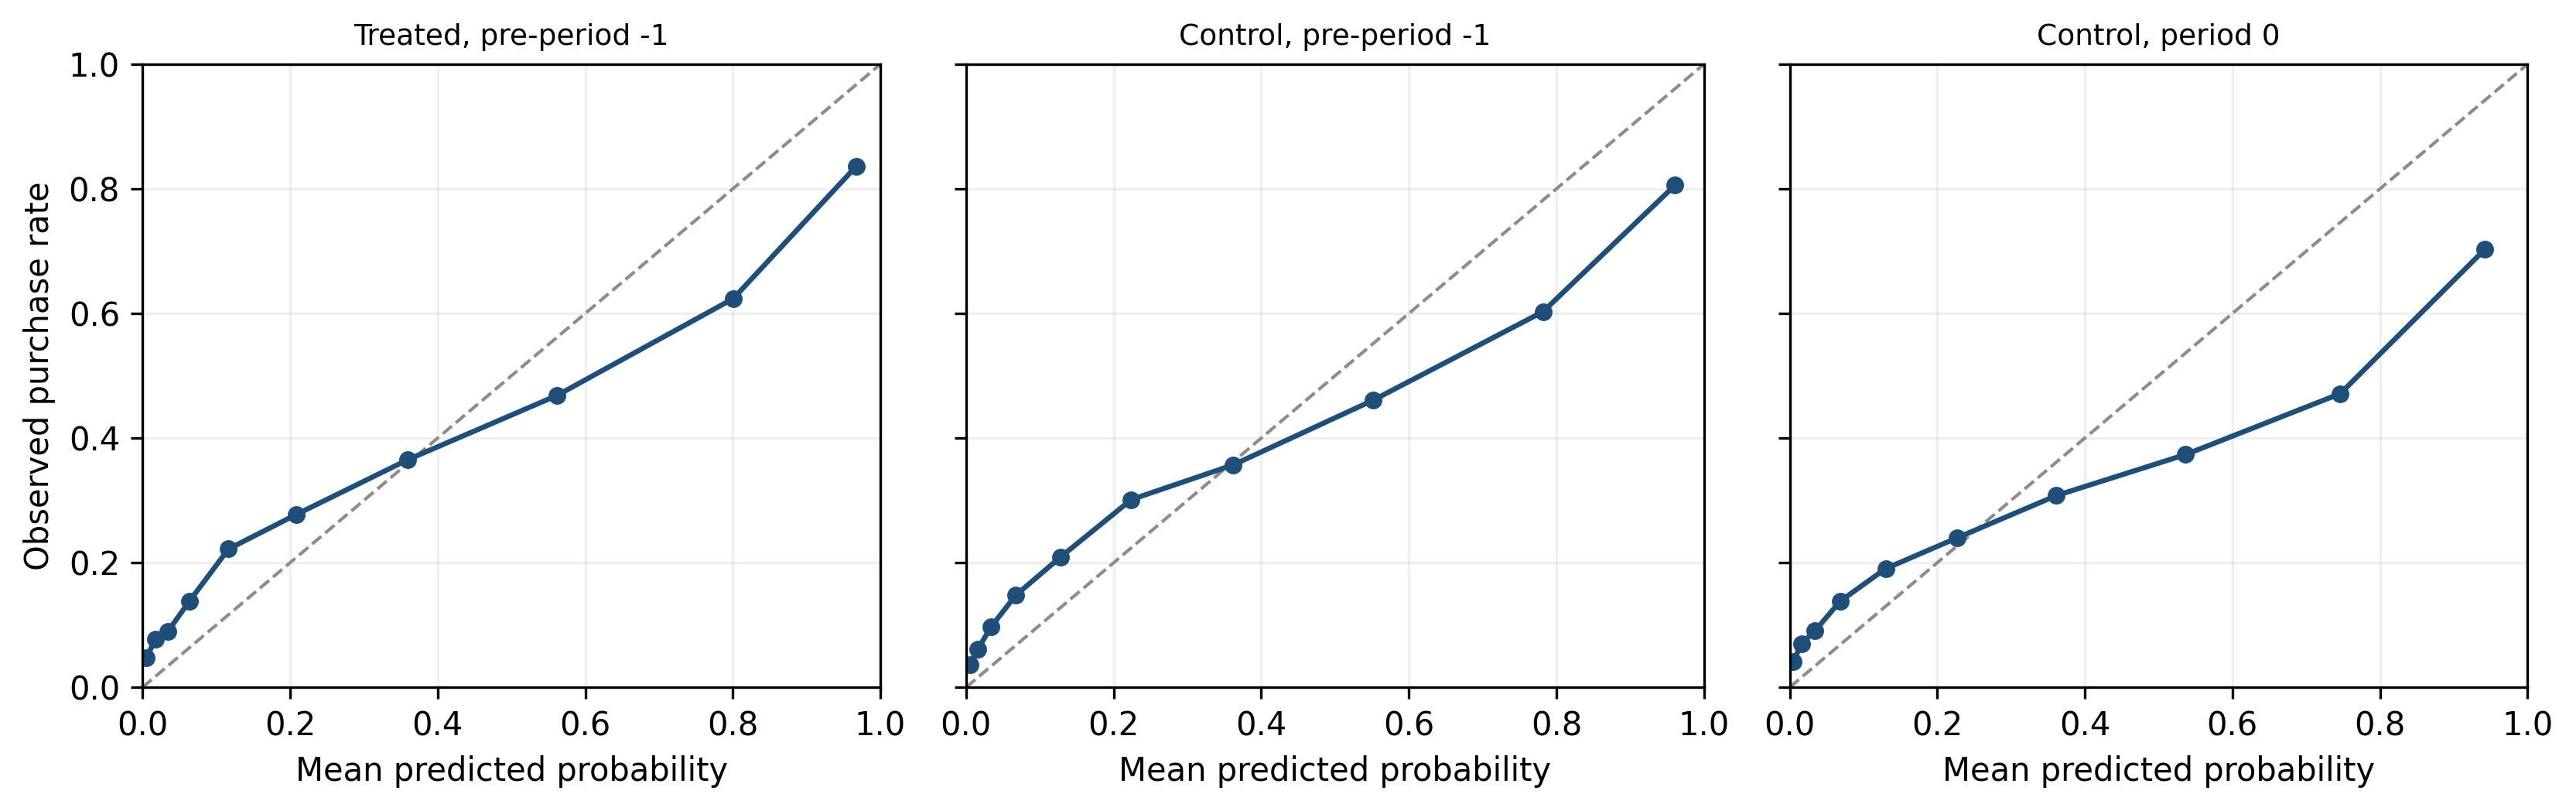
\includegraphics[width=0.98\textwidth]{figures/classifier_calibration.png}
\caption{Calibration of predicted purchase intention}
\label{fig:appendix_classifier_calibration}
\fnote{Notes: Each point is one decile of predicted purchase probability in the exact final cohort. The horizontal coordinate is the decile's mean prediction and the vertical coordinate is its observed purchase rate. The dashed 45-degree line denotes perfect calibration. The flatter empirical paths show that the raw probabilities are too dispersed, although they continue to rank purchase intention.}
\end{figure}

The calibration paths in Figure~\ref{fig:appendix_classifier_calibration} are flatter than the 45-degree line in all three evaluation samples. The model therefore spreads predicted probabilities too widely: observed purchase rates vary less across score deciles than the raw predictions imply. At the same time, observed purchase rates rise with the predicted score, consistent with the ROC-AUC and PR-AUC evidence in the main text that the model meaningfully ranks consumers by purchase propensity. The score is therefore more reliable as a relative ranking than as a perfectly calibrated probability.

Table~\ref{tab:appendix_classifier_duration} evaluates whether this predictive performance is concentrated in closure events of particular lengths.

\begin{table}[!ht]
\centering
\caption{Period-0 control performance by closure duration}
\label{tab:appendix_classifier_duration}
\small
\begin{tabularx}{0.94\textwidth}{Xrrrrrr}
\toprule
Duration & $N$ & Prevalence & ROC-AUC & PR-AUC & Brier & Calibration slope \\
\midrule
10 days & 1,244 & .210 & .774 & .501 & .157 & .461 \\
11 days & 5,020 & .246 & .783 & .585 & .152 & .548 \\
12 days & 3,164 & .196 & .786 & .508 & .154 & .432 \\
13 days & 1,662 & .238 & .780 & .525 & .179 & .388 \\
14 days & 5,232 & .230 & .783 & .555 & .148 & .592 \\
15 days & 551 & .376 & .754 & .686 & .210 & .374 \\
16 days & 2,416 & .300 & .794 & .646 & .176 & .448 \\
17 days & 2,783 & .304 & .789 & .627 & .183 & .478 \\
18 days & 3,176 & .224 & .786 & .569 & .155 & .537 \\
26 days & 4,645 & .299 & .761 & .592 & .208 & .494 \\
28 days & 1,891 & .347 & .791 & .689 & .199 & .489 \\
29 days & 974 & .359 & .739 & .611 & .232 & .331 \\
\bottomrule
\end{tabularx}
\vspace{1mm}
\fnote{Notes: This table evaluates control consumers in period 0 separately for each duration-specific classifier. Duration 25 does not occur in the final 18-event registry and is therefore excluded; it appears only in a broader sensitivity sample. Definitions follow Table~\ref{tab:classifier_diagnostics}.}
\end{table}

Predictive ranking remains informative across all closure durations in Table~\ref{tab:appendix_classifier_duration}. Period-$0$ control ROC-AUC ranges from 0.739 for the 29-day model to 0.794 for the 16-day model, and PR-AUC exceeds the corresponding purchase prevalence in every row. Calibration is consistently weaker: the duration-specific slopes range from 0.331 to 0.592, all below the value of one associated with perfect calibration. No single closure duration therefore drives the classifier's overall ranking performance or its tendency to produce overly dispersed probabilities.

Table~\ref{tab:appendix_classifier_thresholds} shows how the period-$0$ control classification changes when the cutoff varies from .3 to .7.

\begin{table}[!ht]
\centering
\caption{Predictive tradeoffs across classification cutoffs}
\label{tab:appendix_classifier_thresholds}
\small
\begin{tabularx}{0.88\textwidth}{Xrrrrr}
\toprule
Cutoff & Predicted high & Accuracy & Sensitivity & Specificity & PPV \\
\midrule
.30 & .391 & .712 & .695 & .718 & .468 \\
.40 & .325 & .738 & .620 & .780 & .502 \\
.50 & .269 & .756 & .548 & .830 & .534 \\
.60 & .216 & .770 & .474 & .875 & .575 \\
.70 & .170 & .777 & .398 & .911 & .615 \\
\bottomrule
\end{tabularx}
\vspace{1mm}
\fnote{Notes: The evaluation sample is the exact-cohort period-0 controls. Predicted high is the share classified above the stated probability cutoff. These are predictive tradeoffs, not DDD estimates. The main .5 rule is configured before estimation; the continuous-score DDD avoids discretizing the score.}
\end{table}

The cutoff exercise displays the expected sensitivity-specificity tradeoff. Lowering the cutoff from .5 to .3 increases the share classified as high intention from 26.9\% to 39.1\% and raises sensitivity from 0.548 to 0.695, but reduces specificity and positive predictive value. Raising the cutoff to .7 reduces the high-intention share to 17.0\% and increases specificity and positive predictive value to 0.911 and 0.615, while sensitivity falls to 0.398. The .5 rule provides an intermediate classification rather than a uniquely optimal cutoff, which motivates the continuous-score robustness specification.

Figure~\ref{fig:appendix_classifier_overlap} compares the distributions of the predicted period-$0$ score between treated and control consumer-events.

\begin{figure}[!ht]
\centering
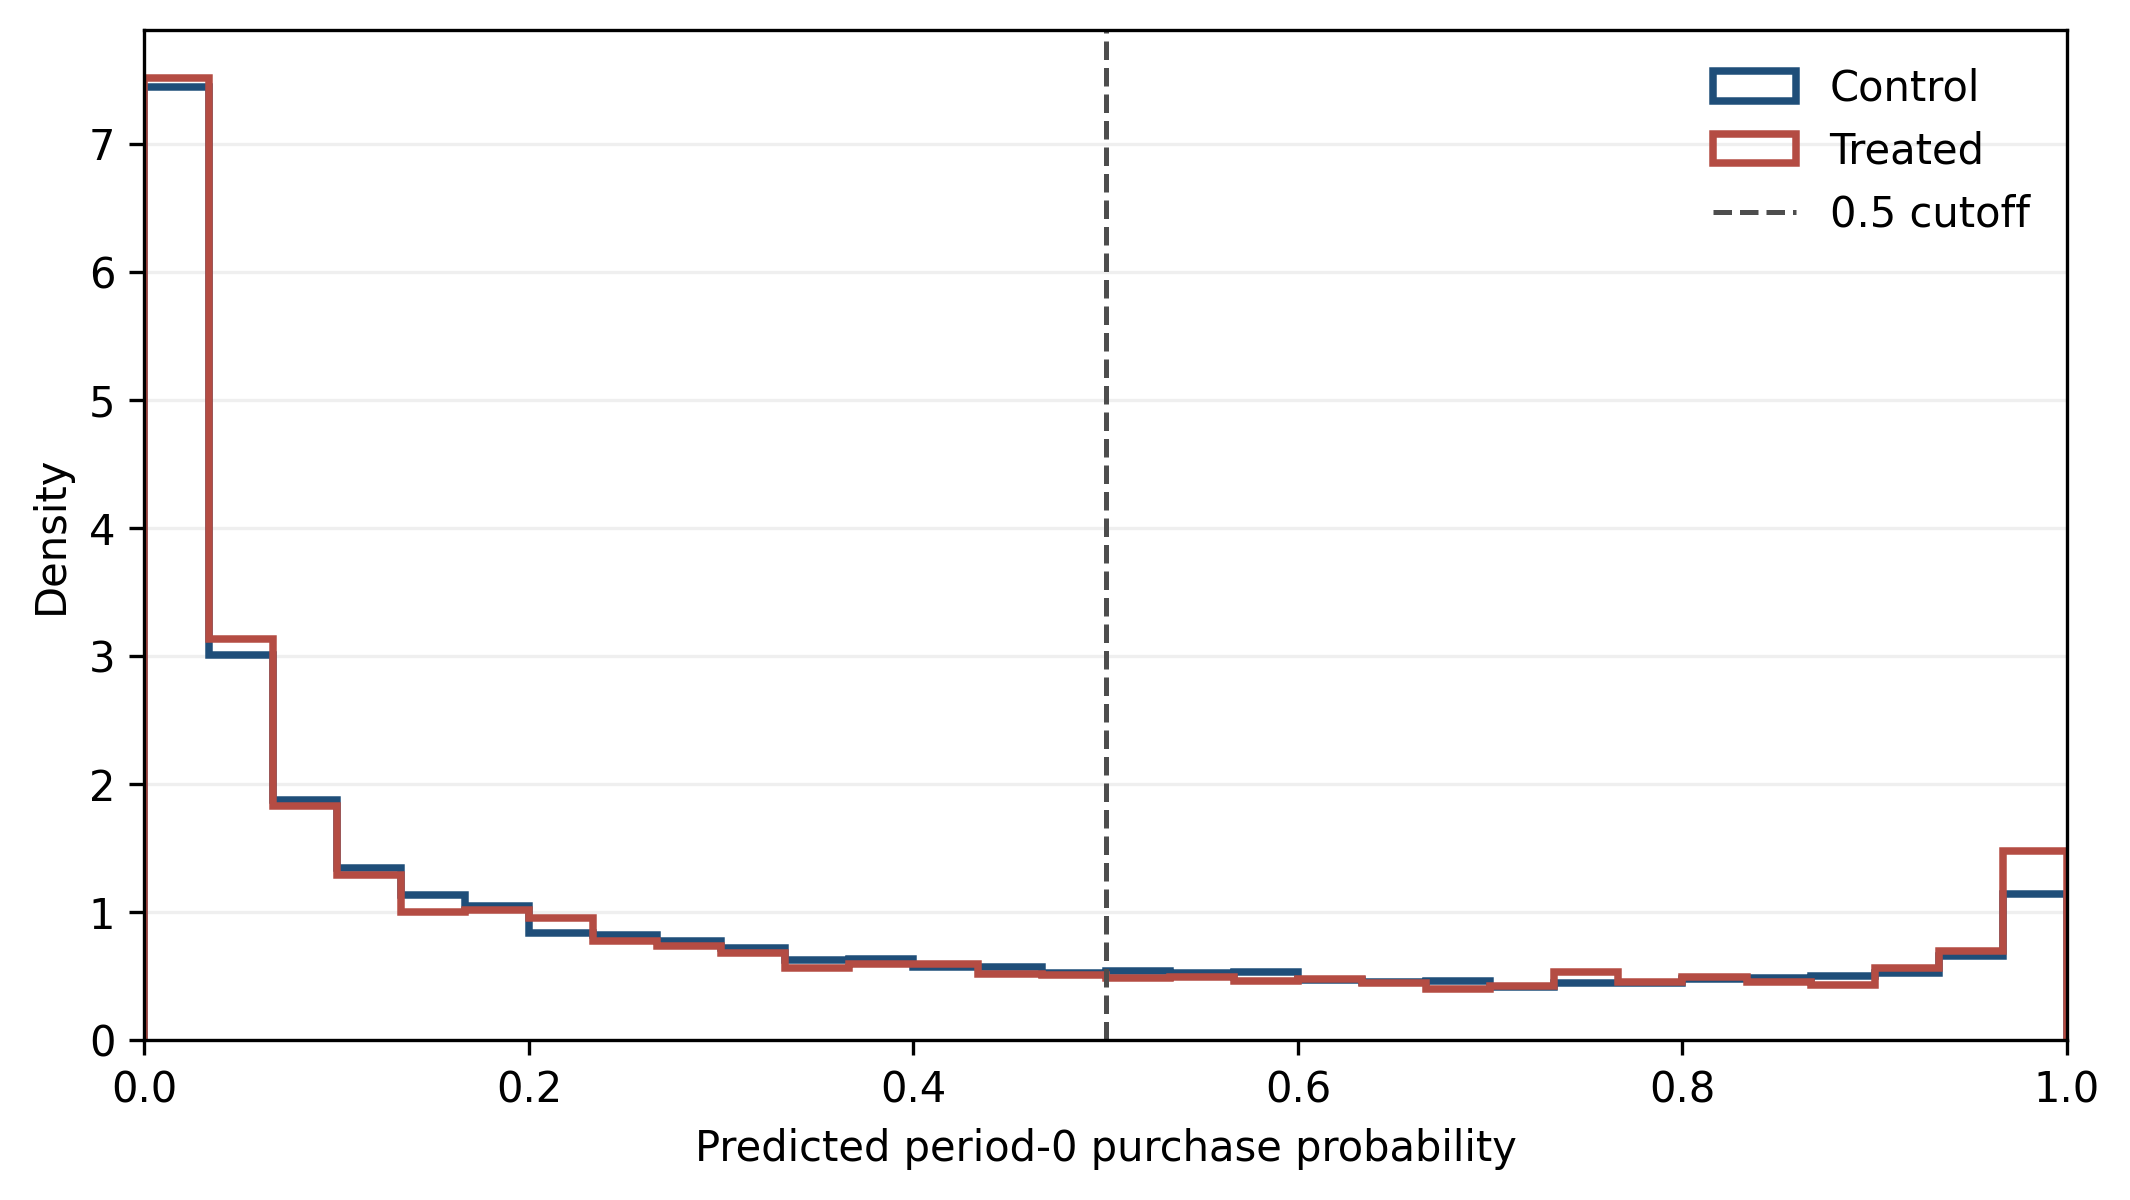
\includegraphics[width=0.76\textwidth]{figures/classifier_score_overlap.png}
\caption{Overlap in predicted period-0 purchase intention}
\label{fig:appendix_classifier_overlap}
\fnote{Notes: The figure shows density histograms of the ex-ante score in the exact final cohort. Mean predicted intention is 0.307 for controls and 0.313 for treated consumers; the median is 0.172 and 0.174, respectively. The shares at or above 0.5 are 26.9\% and 27.6\%. The similar distributions indicate strong score overlap across treatment arms, although overlap does not validate calibration for the unobserved treated period-0 counterfactual.}
\end{figure}

The treated and control score distributions in Figure~\ref{fig:appendix_classifier_overlap} are closely aligned. Their means are 0.313 and 0.307, their medians are 0.174 and 0.172, and 27.6\% and 26.9\% of observations exceed the .5 cutoff, respectively. This overlap indicates that the DDD does not compare treatment groups occupying disjoint regions of the predicted-score distribution. Taken together, the diagnostics show that the classifier ranks purchase propensity reasonably well across closure durations and treatment groups, while calibration is consistently weaker and no cutoff is uniquely preferred. They therefore motivate cautious language for both the binary classification and the continuous-score robustness specification; they do not turn predicted purchase propensity into a direct measure of psychological intention.

\clearpage

\section{Identification Diagnostics}
\label{app:identification_diagnostics}

This appendix reports the formal diagnostics behind the identification discussion in Section~\ref{section:3.3.1}. The main design has three dimensions: treatment exposure, post-reopening timing and predicted purchase intention. The key identifying restriction is therefore a triple-difference restriction: absent the closure, the treated-control gap for high-predicted-intention consumers would have changed like the corresponding gap for low-predicted-intention consumers.

\subsection{Pretrend Tests}
\label{app:pretrend_tests}

For the main novelty-seeking result, we estimate the event-study analog of equation~\eqref{eq:main_ddd}:
\begin{equation}
\begin{split}
Y^N_{iet}={}&\alpha_{ie}+\lambda_t+\gamma_m
+\sum_{\ell\in\{-4,-3,-2,1,2,3,4\}}
\Big[
\delta^B_{\ell}\,\text{Treated}_{ie}
+\beta_{\ell}\,\text{High}_{ie} \\
&\hspace{37mm}
+\delta^D_{\ell}\big(\text{Treated}_{ie}\times\text{High}_{ie}\big)
\Big]\mathbb{1}\{t=\ell\}+\varepsilon_{iet}.
\end{split}
\label{eq:novelty_event_study}
\end{equation}
Period $-1$ is the omitted reference period, and period 0 is the closure window and is excluded. The coefficient $\delta^D_{\ell}$ is the high-minus-low DDD at relative period $\ell$. The pretrend test is the joint null
$H_0:\delta^D_{-4}=\delta^D_{-3}=\delta^D_{-2}=0$.

Table~\ref{tab:appendix_pretrend_tests} reports the three lead coefficients and their joint test for the main novelty-seeking outcome.

\begin{table}[!ht]
\centering
\caption{Novelty-seeking DDD pretrend coefficients and joint test}
\label{tab:appendix_pretrend_tests}
\small
\begin{tabularx}{0.82\textwidth}{Xrrr}
\toprule
\multicolumn{4}{l}{\textit{Panel A: Pre-period high-minus-low DDD coefficients}} \\
Relative period & DDD estimate & SE & 95\% CI \\
\midrule
$-4$ & 2.23 & 2.73 & $[-3.52,\ 7.98]$ \\
$-3$ & 2.64 & 3.44 & $[-4.61,\ 9.90]$ \\
$-2$ & 1.60 & 1.98 & $[-2.57,\ 5.77]$ \\
\addlinespace
\multicolumn{4}{l}{\textit{Panel B: Joint test}} \\
Null hypothesis & Wald statistic & Restrictions & $p$-value \\
\midrule
$\delta^D_{-4}=\delta^D_{-3}=\delta^D_{-2}=0$ & .837 & 3 & .8407 \\
\bottomrule
\end{tabularx}
\vspace{1mm}
\fnote{Notes: Coefficients and standard errors are in percentage points. The dependent variable is novelty-seeking, defined only in windows with a purchase. The regression uses 99,644 observations and includes consumer-event, relative-period and calendar-month fixed effects. Period $-1$ is the omitted reference, and period 0 is excluded. Standard errors are clustered by closure event (18 clusters). The joint Wald test uses the closure-clustered covariance matrix.}
\end{table}

The three novelty-seeking lead estimates in Table~\ref{tab:appendix_pretrend_tests} are positive, between 1.60 and 2.64 percentage points, and each confidence interval includes zero. The joint test does not reject that all three are zero. This is evidence against a pronounced differential pretrend in the observed pre-closure windows, but it does not prove the identifying assumption. Replacing the binary high-intention indicator with the continuous predicted-intention score likewise does not reject a differential pretrend (Wald statistic $=1.781$, $p=0.619$). For transparency about the other outcomes, the purchase-frequency high-minus-low test rejects ($p=0.035$), which is why that result is treated as descriptive, while the new-product-seeking robustness outcome does not reject ($p=0.114$).

Figure~\ref{fig:appendix_novelty_ddd_event_study} shows the novelty high-minus-low coefficient path. The omitted reference period is $-1$, and period 0 is the closure window and is excluded from estimation. Each displayed 95\% confidence interval includes zero. The post-reopening point estimates are negative, but individually imprecise; the figure is therefore evidence about the timing and uncertainty of the response, not a claim that every post-period coefficient differs from zero.

\begin{figure}[!ht]
\centering
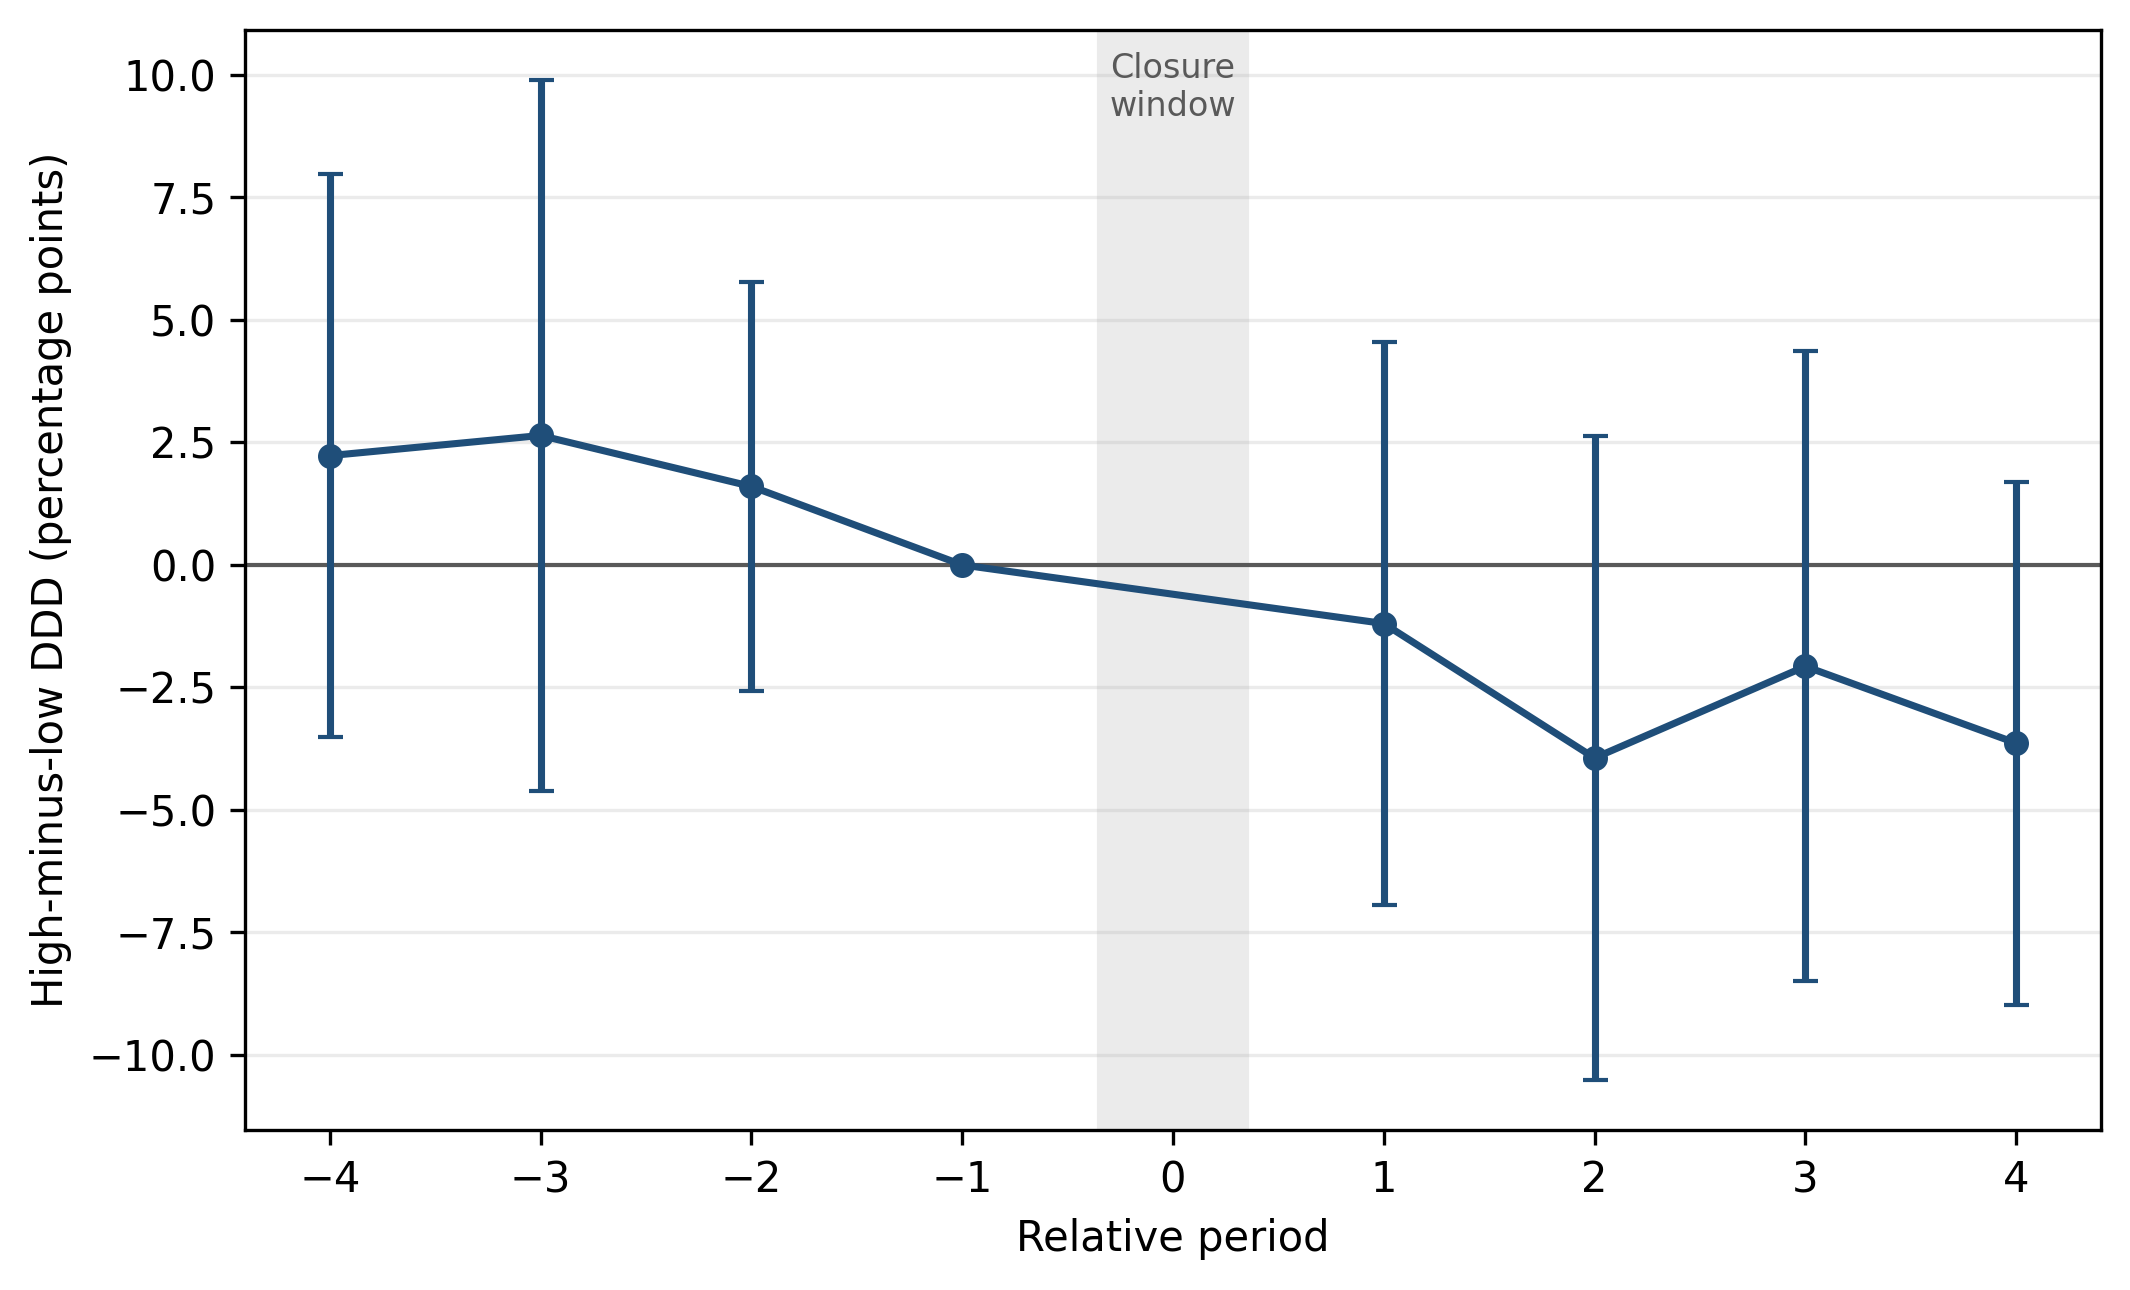
\includegraphics[width=0.86\textwidth]{figures/novelty_ddd_event_study.png}
\caption{Event-study path of the novelty-seeking DDD}
\label{fig:appendix_novelty_ddd_event_study}
\fnote{Notes: Points are the event-study coefficients on Treated $\times$ High predicted intention relative to period $-1$. Vertical bars use the confidence limits reported by the closure-event-clustered estimator (18 clusters). Period 0 is the closure window and is omitted. Novelty-seeking is conditional on a purchase in the window.}
\end{figure}

\begin{comment}
\subsection{Common-Support Sensitivity}
\label{app:common_support}

The identifying comparison can be strained when high- and low-predicted-intention consumers have different pre-period demand. We therefore construct a deterministic common-support sample separately within treated and control consumers. Coarsened cells use mean and most recent pre-period purchase frequency and purchase recency; the novelty match additionally uses pre-period purchase intention because novelty is defined only in purchasing windows. Within each cell, we retain equal numbers of high- and low-predicted-intention consumers. Table~\ref{tab:appendix_common_support} compares the full-sample DDDs with estimates from the resulting common-support samples.

\begin{table}[!ht]
\centering
\caption{Common-support sensitivity of the DDD estimates}
\label{tab:appendix_common_support}
\small
\begin{tabularx}{\textwidth}{Xcccc}
\toprule
 & \multicolumn{2}{c}{Full sample} & \multicolumn{2}{c}{Matched common support} \\
\cmidrule(lr){2-3}\cmidrule(lr){4-5}
Outcome & DDD & Observations & DDD & Observations \\
\midrule
Purchase frequency & \textbf{.0058} & 321,184 & \textbf{-.0041} & 101,072 \\
 & (.0032) & & (.0027) & \\
 & [.0860] & & [.1561] & \\
Novelty-seeking & \textbf{-.0415} & 99,644 & \textbf{-.0211} & 43,655 \\
 & (.0184) & & (.0195) & \\
 & [.0380] & & [.2955] & \\
\bottomrule
\end{tabularx}
\vspace{1mm}
\fnote{Notes: The table reports the high-minus-low DDD, with all DDD coefficients shown in boldface. The matched sample imposes common support between high- and low-predicted-intention consumers separately within treated and control groups using the coarsened cells described in the text. Standard errors, clustered by closure event (18 clusters), are in parentheses; p-values are in brackets. The matched estimates are sensitivity diagnostics rather than preferred estimates.}
\end{table}

The support restriction retains 12,634 of 40,148 consumer-events for purchase frequency and 10,956 consumer-events for novelty-seeking before the product-choice singleton restriction. As Table~\ref{tab:appendix_common_support} shows, the purchase-frequency DDD changes sign and is imprecise ($p=0.156$); its matched-sample DDD pretrend also does not reject at 5\% but is borderline ($p=0.069$). The novelty DDD is about half the full-sample magnitude and is imprecise ($p=0.295$), while its matched pretrend does not reject ($p=0.871$). The common-support exercise therefore does not provide affirmative robustness: it shows that the headline estimates, especially purchase frequency, are sensitive to restricting the comparison to closely aligned pre-period demand cells.
\end{comment}

\subsection{Dynamics of Baseline-Novelty Heterogeneity}
\label{app:baseline_novelty_dynamics}

The collapsed heterogeneity estimate in Table~\ref{tab:baseline_novelty_heterogeneity} compares all four post-reopening periods with all four pre-closure periods. Figure~\ref{fig:appendix_baseline_novelty_event_study} replaces the collapsed post indicator with relative-period interactions, retaining the same fixed effects, baseline-order adjustment and closure-event clustering. The omitted reference period is $-1$.

The three lead coefficients are small relative to their confidence intervals, and their joint test does not reject equality to zero ($p=0.561$). The post-period gradients are positive in periods 1, 3 and 4 and near zero in period 2. The largest estimate occurs immediately after reopening, but every period-specific 95\% confidence interval includes zero. The figure therefore supports the absence of a pronounced differential pretrend while also showing that the timing of the mechanism result is imprecisely estimated.

\begin{figure}[!ht]
\centering
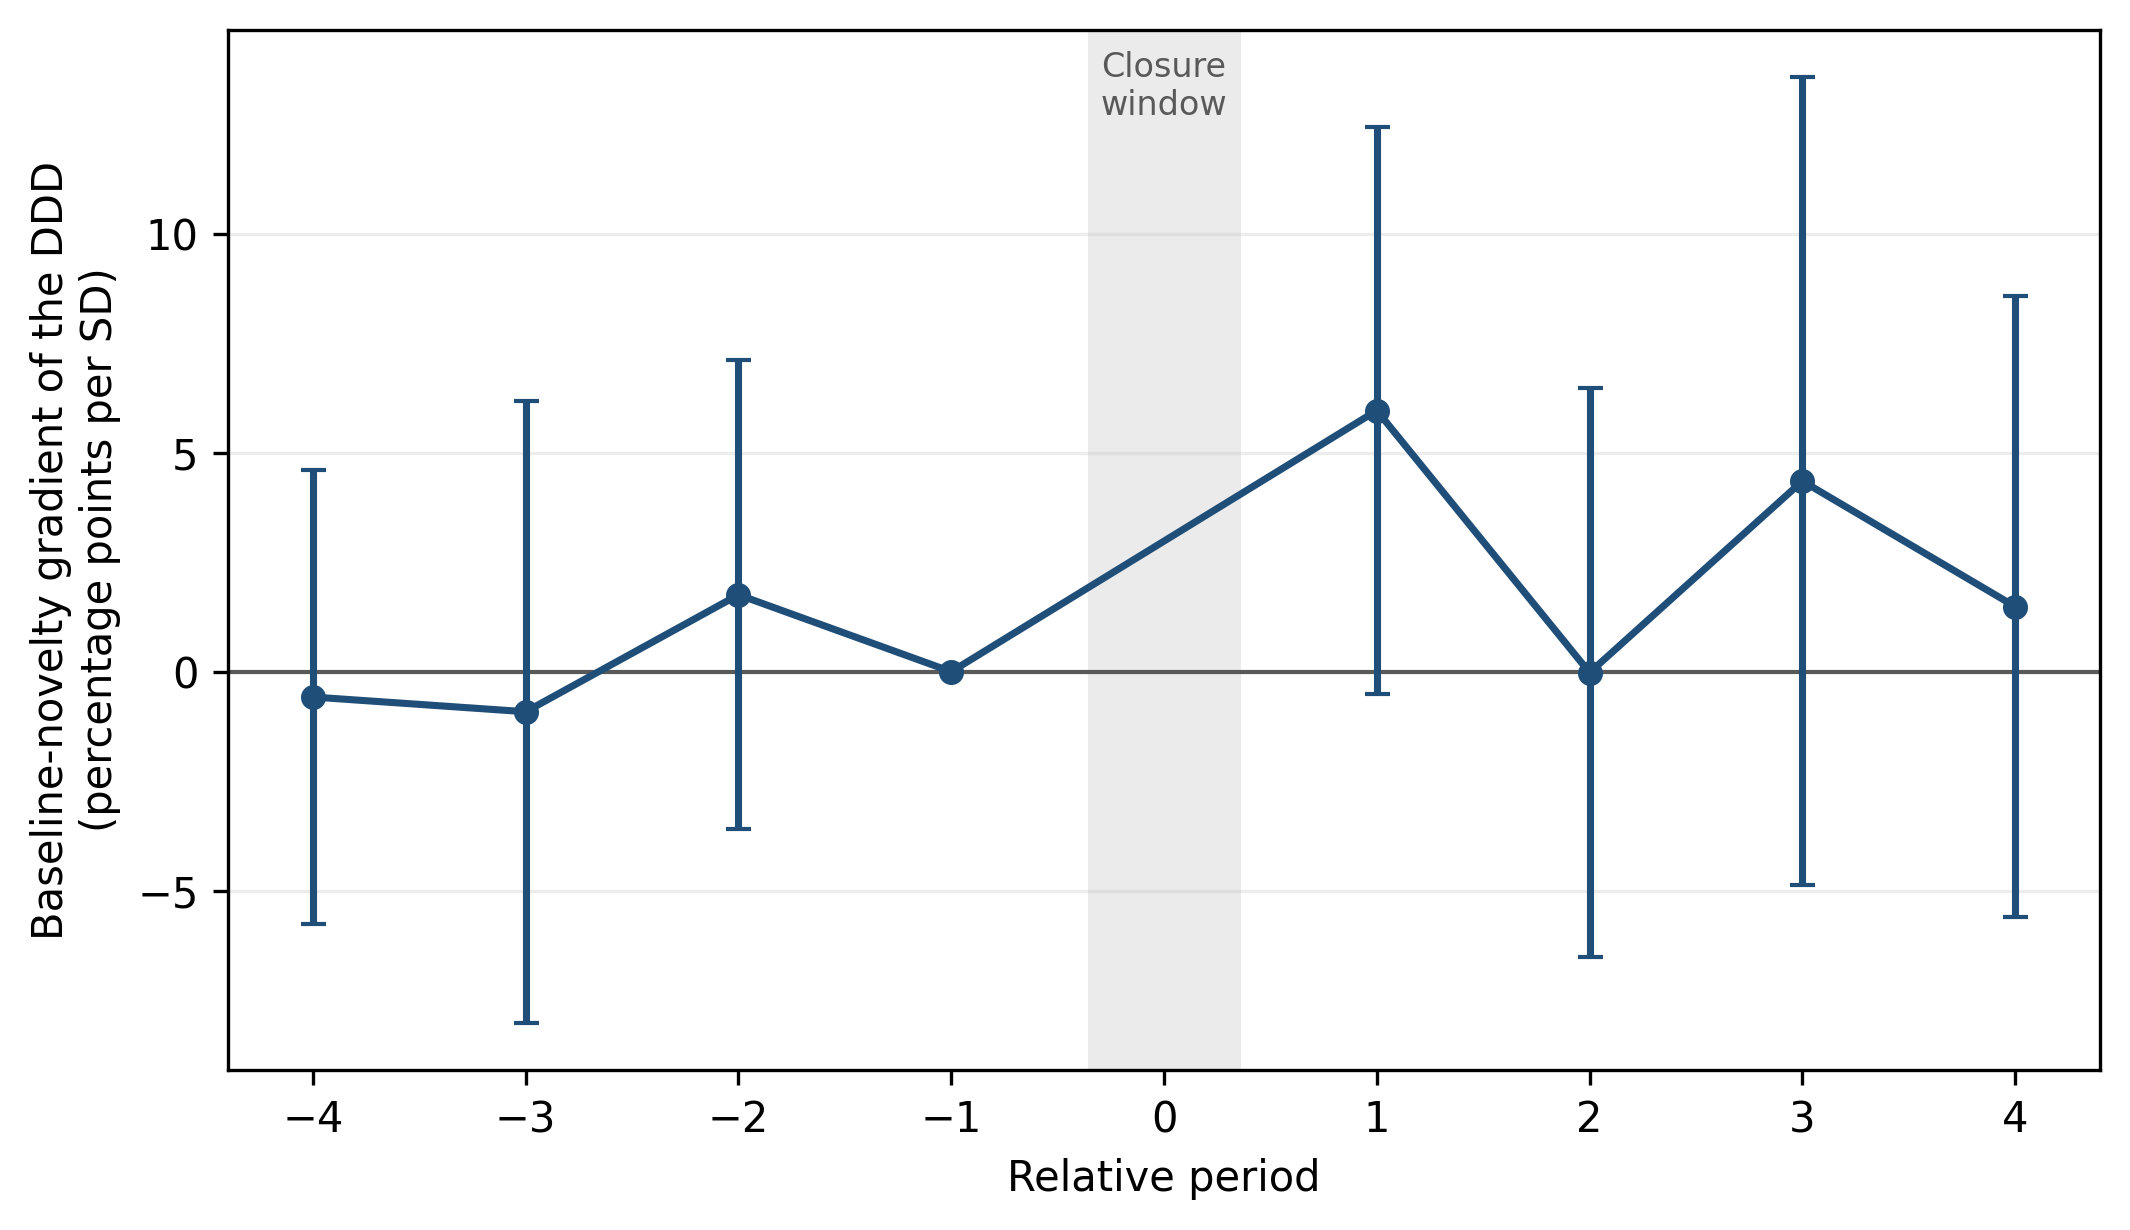
\includegraphics[width=0.86\textwidth]{figures/baseline_novelty_event_study.png}
\caption{Event-study path of the baseline-novelty gradient}
\label{fig:appendix_baseline_novelty_event_study}
\fnote{Notes: Points are coefficients on Relative period $\times$ Treated $\times$ High predicted intention $\times$ standardized baseline novelty-seeking. Vertical bars are 95\% confidence intervals from CRV1 standard errors clustered by closure event (18 clusters). Relative period $-1$ is the omitted reference period; period 0 is the closure window and is excluded. The specification includes the full lower-order interaction hierarchy for baseline novelty and the parallel hierarchy for standardized log baseline orders, as in equation~\eqref{eq:baseline_novelty_heterogeneity}.}
\end{figure}

\section{Alternative Explanations}
\label{app:alternative_explanations}
\subsection{New-Product Notification Exposure}
\label{app:new_product_notifications}

This section reports the construction and estimates behind Section~\ref{section:alternative_new_product_notifications}. The raw files contain 56,724,521 push records. We retain the 40,148 consumer-events in the 18-closure analysis and map notifications into the four event-length periods before closure, the closure window and the four event-length periods after reopening. This produces a balanced panel of 361,332 consumer-event-period observations. Of the 912,911 push records mapped into these windows, 125,918 have \texttt{trigger\_tag}=3, the platform classification for a new-product notification.

The primary measure counts unique consumer-policy-date notification campaigns and divides by the number of calendar days in the event window. All 125,918 new-product records are unique at this grain, so the campaign and raw-record measures coincide. Supporting outcomes indicate whether a consumer receives any new-product notification, count distinct notification days and measure the share of all campaigns classified as new-product notifications. The source files record targeting entries; they do not verify delivery, impression, opening or reading.

For exposure outcome $N_{iet}$, we estimate
\begin{equation}
	N_{iet}=\beta_1(\text{After}_{et}\times\text{Treated}_{i})
	+\beta_2(\text{After}_{et}\times\text{High}_{i})
	+\beta_3(\text{After}_{et}\times\text{Treated}_{i}\times\text{High}_{i})
	+\phi_{ie}+\omega_t+\gamma_m+\varepsilon_{iet},
	\label{eq:new_product_notification_ddd}
\end{equation}
where $\text{After}_{et}$ denotes either the closure window or the post-reopening periods. The closure specification compares period 0 with all four pre-periods; a sensitivity check compares it only with period $-1$. The post specification omits period 0 and compares the four post-periods with the four pre-periods, as in the main outcome regression. Standard errors are clustered by closure event. Because there are 18 clusters, Table~\ref{tab:appendix_new_product_notifications} also reports restricted wild-cluster $p$-values for $\beta_3$.

\begin{table}[!ht]
\centering
\caption{Differential exposure to new-product notifications}
\label{tab:appendix_new_product_notifications}
\scriptsize
\begin{tabularx}{\textwidth}{Xccc}
\toprule
 & During versus all pre-periods & During versus period $-1$ & Post versus pre-periods \\
 & (1) & (2) & (3) \\
\midrule
New-product campaigns per day & $0.0041$ & $0.0043$ & $0.0017$ \\
 & $(0.0011)$ & $(0.0013)$ & $(0.0007)$ \\
Restricted wild-cluster $p$-value & $[0.0032]$ & $[0.0111]$ & $[0.0469]$ \\
\addlinespace
Any new-product notification & $0.0422$ & $0.0362$ & $0.0144$ \\
 & $(0.0100)$ & $(0.0110)$ & $(0.0061)$ \\
Restricted wild-cluster $p$-value & $[0.0010]$ & $[0.0057]$ & $[0.0399]$ \\
\addlinespace
New-product notification days per day & $0.0041$ & $0.0043$ & $0.0017$ \\
 & $(0.0011)$ & $(0.0013)$ & $(0.0007)$ \\
Restricted wild-cluster $p$-value & $[0.0031]$ & $[0.0111]$ & $[0.0471]$ \\
\addlinespace
All campaigns per day & $0.0230$ & $0.0143$ & $0.0113$ \\
 & $(0.0087)$ & $(0.0078)$ & $(0.0058)$ \\
Restricted wild-cluster $p$-value & $[0.0823]$ & $[0.1648]$ & $[0.1104]$ \\
\addlinespace
New-product share of campaigns & $0.0020$ & $-0.0014$ & $-0.0005$ \\
 & $(0.0095)$ & $(0.0057)$ & $(0.0058)$ \\
Restricted wild-cluster $p$-value & $[0.8505]$ & $[0.8080]$ & $[0.9406]$ \\
\addlinespace
Observations, primary outcome & 200,740 & 80,296 & 321,184 \\
Closure-event clusters & 18 & 18 & 18 \\
\bottomrule
\end{tabularx}
\vspace{1mm}
\fnote{Notes: Entries are coefficients on $\text{After}\times\text{Treated}\times\text{High}$ from equation~\eqref{eq:new_product_notification_ddd}. A negative coefficient is required for the proposed notification explanation. Standard errors clustered by closure event are in parentheses; restricted wild-cluster $p$-values are in brackets. All specifications include consumer-event, relative-period and calendar-month fixed effects. The campaign-share regressions are conditional on receiving at least one campaign and use 107,606, 39,628 and 183,480 observations in columns (1)--(3), respectively.}
\end{table}

Table~\ref{tab:appendix_new_product_notifications} shows that the differential change in recorded new-product campaigns is positive rather than negative. Relative exposure among treated high-intention consumers increases by 0.0041 campaigns per day during the closure when all pre-periods form the comparison ($p=0.003$) and by 0.0043 when period $-1$ alone forms the comparison ($p=0.011$). The differential remains positive after reopening at 0.0017 campaigns per day ($p=0.047$). The indicators for receiving any new-product notification and the number of notification days produce the same positive pattern. Total campaign frequency also rises, although its wild-cluster $p$-values exceed 0.05, while the new-product share of all campaigns remains close to zero in every comparison. The increase in new-product notifications therefore reflects a broader increase in recorded campaign targeting rather than a larger new-product share, and none of the specifications produces the negative differential required by the notification explanation.

Table~\ref{tab:appendix_new_product_notification_dynamics} reports the dynamic specification, which replaces $\text{After}$ with relative-period indicators and omits period $-1$. The three lead estimates are individually small, and their joint test does not reject equality to zero ($p=0.500$). The coefficient is largest during closure, remains positive in the first reopening period and then declines. This timing is consistent with high-intention treated consumers becoming newly eligible for inactivity-triggered campaigns when a likely purchase is interrupted. It is inconsistent with the negative differential exposure needed to explain the novelty DDD.

\begin{table}[!ht]
\centering
\caption{Event-study path of new-product notification exposure}
\label{tab:appendix_new_product_notification_dynamics}
\small
\begin{tabular}{lccc}
\toprule
Relative period & Coefficient & Standard error & $p$-value \\
\midrule
$-4$ & $0.0007$ & $(0.0010)$ & $[0.466]$ \\
$-3$ & $-0.0002$ & $(0.0012)$ & $[0.878]$ \\
$-2$ & $0.0002$ & $(0.0009)$ & $[0.800]$ \\
$0$ & $0.0043$ & $(0.0013)$ & $[0.004]$ \\
$1$ & $0.0031$ & $(0.0013)$ & $[0.036]$ \\
$2$ & $0.0015$ & $(0.0011)$ & $[0.185]$ \\
$3$ & $0.0022$ & $(0.0011)$ & $[0.064]$ \\
$4$ & $0.0003$ & $(0.0008)$ & $[0.712]$ \\
\addlinespace
Joint pretrend $p$-value & \multicolumn{3}{c}{$0.500$} \\
\bottomrule
\end{tabular}
\vspace{1mm}
\fnote{Notes: The outcome is unique new-product notification campaigns per consumer-day. Coefficients are relative-period $\times$ Treated $\times$ High interactions relative to period $-1$. Standard errors use CRV1 clustering by the 18 closure events. Period 0 is the closure window.}
\end{table}

The inactivity pattern in the records also clarifies why absolute high-low levels are not informative. Among treated consumers, the median new-product notification occurs 121 days after the last purchase for low-intention consumers before closure and 129 days during closure. The corresponding medians for high-intention consumers are 56 and 40 days. Low-intention consumers therefore receive more notifications in levels because they are ordinarily more dormant. The DDD removes this persistent gap and shows that the relative exposure increase occurs among treated high-intention consumers instead.


\subsection{Reopening Assortment}
\label{app:reopening_assortment}

This section reports the construction and estimates behind the assortment test in Section~\ref{section:alternative_assortment}. The alternative explanation is that high- and low-intention consumers may return at different times after a treated store reopens and therefore encounter different product assortments. For differences in return timing to generate differences in product choice, however, the assortment available at the store must itself vary systematically with time since reopening. We therefore focus first on the evolution of realized assortment at the 18 treated stores during the first four weeks after reopening.

For each closure, we construct four fixed seven-day periods beginning immediately after reopening. Fixed weeks provide a common measure of time since reopening across events even though the preceding closures last between 10 and 29 days. We construct three measures from product-level transactions. \textit{Core-product coverage} defines a store's core set as products sold in at least three of the four weeks before closure and measures the share of that set sold in each post-reopening week. \textit{Products per 50 baskets} draws 50 consumer-day baskets without replacement, counts the number of distinct products, and averages this count over 100 draws. This rarefaction holds observed basket volume fixed; store-weeks with fewer than 50 baskets are missing. \textit{Pre-menu overlap} is the Jaccard similarity between products sold in a store-week and the union of products sold in that store's four pre-closure weeks. These measures capture different dimensions of the realized product assortment while avoiding a mechanical interpretation of lower transaction volume as lower product availability.

\paragraph{Assortment evolution after reopening.}
For assortment outcome $A_{et}$ at treated store associated with closure event $e$ in post-reopening week $t$, we estimate
\begin{equation}
A_{et}
=
\alpha_e
+
\sum_{k=2}^{4}\beta_k
\mathbb{1}{t=k}
+
\varepsilon_{et},
\label{eq:assortment_post_path}
\end{equation}
where week 1 is the omitted category and $\alpha_e$ denotes closure-event fixed effects. The coefficients $\beta_k$ therefore measure how realized assortment in weeks 2--4 differs from the first week after reopening. We test the joint null
\[
H_0:\beta_2=\beta_3=\beta_4=0,
\]
which corresponds to no systematic change in the assortment across the four post-reopening weeks. Table~\ref{tab:appendix_reopening_assortment_post} reports the weekly coefficients and joint tests for all three measures.

\begin{table}[!ht]
\centering
\caption{Evolution of realized assortment after reopening}
\label{tab:appendix_reopening_assortment_post}
\small
\begin{tabularx}{\textwidth}{Xccc}
\toprule
& Core-product coverage & Products per 50 baskets & Pre-menu overlap \\
& (1) & (2) & (3) \\
\midrule
Week 2 relative to week 1 & $0.0059$ & $0.3019$ & $-0.0100$ \\
& $(0.0185)$ & $(0.7351)$ & $(0.0129)$ \\
Week 3 relative to week 1 & $-0.0648$ & $-0.7031$ & $-0.0763$ \\
& $(0.0544)$ & $(0.6006)$ & $(0.0410)$ \\
Week 4 relative to week 1 & $-0.0840$ & $-1.6600$ & $-0.1111$ \\
& $(0.0537)$ & $(0.5552)$ & $(0.0403)$ \\
\addlinespace
Joint equality test, $p$-value & $0.3821$ & $0.0106$ & $0.0175$ \\
Week 1 mean & $0.7687$ & $29.2581$ & $0.6120$ \\
Observations & 72 & 64 & 72 \\
Treated stores & 18 & 16 & 18 \\
\bottomrule
\end{tabularx}

\vspace{1mm}
\fnote{Notes: The sample contains the treated stores during the first four fixed seven-day periods after reopening. Core-product coverage is the share of products in the store's core pre-closure set that sell in the current week. Products per 50 baskets averages the number of distinct products across 100 samples of 50 consumer-day baskets drawn without replacement. Pre-menu overlap is the Jaccard similarity between products sold in the current week and the store's pre-closure product set. Week 1 is the omitted category in equation~\eqref{eq:assortment_post_path}. Standard errors in parentheses use CRV1 clustering by closure event. The joint row reports restricted Rademacher wild-cluster $p$-values based on 9,999 replications for the null that the coefficients for weeks 2, 3, and 4 are jointly zero. Columns (1) and (3) contain all 18 treated stores; column (2) requires at least 50 baskets in every week and therefore contains 16.}
\end{table}

Table~\ref{tab:appendix_reopening_assortment_post} shows no statistically detectable change in core-product coverage: relative to week 1, the estimates are $+0.59$, $-6.48$, and $-8.40$ percentage points in weeks 2--4, and the joint test yields $p=0.382$. Standardized product breadth first increases by 0.30 products per 50 baskets and then falls by 0.70 and 1.66 products, with a joint $p$-value of 0.011. Pre-menu overlap similarly declines by 1.00, 7.63, and 11.11 percentage points, and its joint test rejects a constant path ($p=0.018$). Assortment stability alone therefore cannot rule out differential return timing.

\paragraph{Return timing and consumer-specific novel opportunity.}
We next test the channel directly among treated consumers. A returner is a treated consumer whose first purchase at the reopened focal store occurs within 28 days of reopening. Of 5,349 low-intention and 2,041 high-intention treated consumers, 1,134 (21.2\%) and 1,268 (62.1\%), respectively, return within this window. High-intention returners return 2.87 days earlier after conditioning on closure-event fixed effects (SE $=0.29$; $p<0.001$). Their median return is day 7 rather than day 11, and 53.6\% return in week 1 compared with 36.9\% of low-intention returners.

For each returner, we construct the realized product set in each of the four candidate return weeks. To prevent the consumer's observed purchase from mechanically entering the opportunity set, we remove any product sold only to that consumer in the store-week; products also purchased by another consumer remain. We define a product as personally novel if the consumer had not purchased it by the reopening date. Let $M_{iew}$ denote either the leave-one-consumer-out novel-product share or count for consumer $i$, event $e$, and candidate return week $w$. Our timing measure is
\begin{equation}
D_{ie}=M_{ie,w(i)}-\frac{1}{4}\sum_{w=1}^{4}M_{iew},
\label{eq:assortment_timing_exposure}
\end{equation}
where $w(i)$ is the consumer's actual return week. Subtracting the same consumer's four-week mean removes persistent high--low differences in product history and retains only the opportunity change associated with returning in one week rather than another. We regress $D_{ie}$ on the high-intention indicator and closure-event fixed effects, clustering by closure event. Table~\ref{tab:appendix_reopening_assortment_timing} reports the return-time difference together with the resulting differences in personally novel product opportunity.

\begin{table}[H]
\centering
\caption{Return timing and personally novel product opportunity}
\label{tab:appendix_reopening_assortment_timing}
\small
\begin{tabularx}{\textwidth}{Xccc}
\toprule
& Days to first return & Novel-product share & Novel-product count \\
& (1) & (2) & (3) \\
\midrule
High minus low intention & $-2.8724$ & $-0.0010$ & $-0.2756$ \\
& $(0.2936)$ & $(0.0006)$ & $(0.3848)$ \\
& $[<0.001]$ & $[0.0930]$ & $[0.4836]$ \\
\addlinespace
Low-intention mean & $12.1570$ & $-0.0005$ & $1.5780$ \\
High-intention mean & $9.0331$ & $-0.0016$ & $1.0562$ \\
Observations & 2,402 & 2,325 & 2,402 \\
Closure-event clusters & 18 & 17 & 18 \\
\bottomrule
\end{tabularx}
\vspace{1mm}
\fnote{Notes: The sample contains treated consumers whose first focal-store purchase occurs within 28 days after reopening. Column (1) reports days from reopening to that purchase. Columns (2) and (3) report the timing deviations in equation~\eqref{eq:assortment_timing_exposure}; means in those columns are therefore deviations from each consumer's four-week average opportunity, not levels. The share is the fraction of the leave-one-consumer-out realized product set that the consumer had never purchased by reopening, and the count is the number of such products. The share analysis requires a nonempty leave-one-consumer-out product set in all four weeks. All specifications include closure-event fixed effects. Standard errors clustered by closure event are in parentheses, and two-sided $p$-values are in brackets.}
\end{table}

Table~\ref{tab:appendix_reopening_assortment_timing} confirms that high-intention returners return 2.87 days earlier on average. Their mean return time is 9.03 days, compared with 12.16 days for low-intention returners. Despite this timing difference, the high-minus-low deviation is only $-0.10$ percentage points for the novel-product share (95\% CI: $-0.22$ to $+0.02$) and $-0.28$ products for the count (95\% CI: $-1.09$ to $+0.54$). The share estimate has the direction required by the alternative explanation but is only about one-fortieth of the $-4.15$-percentage-point main novelty DDD, and its confidence interval excludes effects comparable to that magnitude. The count estimate is statistically indistinguishable from zero and small relative to roughly 67 personally novel products in the realized return-week sets. Differential return timing therefore produces too little differential exposure to personally novel products to account quantitatively for the main result in the observed transaction environment.

\paragraph{Comparison with matched control stores.}
As an additional check, we examine whether treated stores experience an unusual change in realized assortment relative to their matched control stores. This analysis uses the 18 treated stores and their five matched control stores and constructs four fixed seven-day periods before closure and four fixed seven-day periods after reopening. For assortment outcome $A_{est}$ at store $s$, event $e$, and relative week $t$, we estimate
\begin{equation}
A_{est}
=
\beta\big(\text{TreatedStore}_{es}\times\text{Post}_{et}\big)
+\alpha_{es}
+\lambda_{et}
+\varepsilon_{est},
\label{eq:assortment_did}
\end{equation}
where $\alpha_{es}$ denotes event-store fixed effects and $\lambda_{et}$ denotes event-by-relative-week fixed effects. The specification compares the change in assortment at the treated store with the contemporaneous change among its matched controls.

Table~\ref{tab:appendix_reopening_assortment} reports no evidence of a relative contraction after reopening. Core-product coverage falls by 1.29 percentage points more at treated stores than at controls (SE $=3.41$ percentage points; $p=0.710$). Standardized product breadth increases by 0.31 products per 50 baskets (SE $=0.52$; $p=0.562$), while pre-menu overlap increases by 1.46 percentage points (SE $=2.50$ percentage points; $p=0.567$). The immediate-reopening estimates are also not statistically distinguishable from zero for any measure. The joint pretrend tests yield $p$-values of 0.110, 0.412, and 0.522 for core-product coverage, product breadth, and pre-menu overlap, respectively. Thus, neither the collapsed estimates nor the event-study comparisons show a common relative post-reopening decline at treated stores.

\begin{table}[!ht]
\centering
\caption{Realized assortment at reopening stores and matched controls}
\label{tab:appendix_reopening_assortment}
\small
\begin{tabularx}{\textwidth}{Xccc}
\toprule
& Core-product coverage & Products per 50 baskets & Pre-menu overlap \\
& (1) & (2) & (3) \\
\midrule
Post $\times$ Treated store & $-0.0129$ & $0.3063$ & $0.0146$ \\
& $(0.0341)$ & $(0.5178)$ & $(0.0250)$ \\
& $[0.7097]$ & $[0.5619]$ & $[0.5665]$ \\
\addlinespace
Immediate reopening, relative to week $-1$ & $0.0205$ & $0.1935$ & $0.0495$ \\
& $(0.0365)$ & $(0.8753)$ & $(0.0293)$ \\
& $[0.5806]$ & $[0.8277]$ & $[0.1097]$ \\
Joint pretrend $p$-value & $0.1103$ & $0.4123$ & $0.5218$ \\
Control pre-period mean & $0.9240$ & $28.2045$ & $0.7513$ \\
Observations & 736 & 723 & 736 \\
Event-store pairs & 92 & 92 & 92 \\
Closure-event clusters & 18 & 18 & 18 \\
\bottomrule
\end{tabularx}
\vspace{1mm}
\fnote{Notes: Core-product coverage is the share of products in a store's core pre-closure set that sell in the current week. Products per 50 baskets averages the number of distinct products across 100 samples of 50 consumer-day baskets drawn without replacement. Pre-menu overlap is the Jaccard similarity between products sold in the current week and the store's pre-closure product set. Standard errors clustered by the 18 closure events are in parentheses, and two-sided $p$-values are in brackets. Product sales measure realized assortment and need not equal the product set displayed or available to every consumer.}
\end{table}

The matched-store analysis addresses a different question from the return-timing test. It asks whether closure and reopening are associated with an unusual store-level assortment change relative to contemporaneous controls. The four-week path shows that realized assortment subsequently evolves, so the direct test of the alternative is instead the consumer-specific timing deviation in equation~\eqref{eq:assortment_timing_exposure}. The transaction data cannot reveal the exact product set presented to each consumer, and the return analysis is descriptive among consumers who return within 28 days. Subject to these limitations, the observed timing-induced differences are too small to account quantitatively for the main novelty result.

\clearpage


\section{Additional Results}
\label{app:additional_results}

\subsection{Complete Main Specifications}
\label{app:complete_main_results}

The main text reports the group-specific effects and DDDs that carry the economic interpretation. This section reports the full coefficient vectors from the underlying regressions. Table~\ref{tab:appendix_binary_main_results} presents equation~\eqref{eq:main_ddd} for the two main outcomes.

\begin{table}[!ht]
\centering
\caption{Complete binary predicted-intention specifications}
\label{tab:appendix_binary_main_results}
\small
\begin{tabularx}{\textwidth}{Xcc}
\toprule
 & Purchase frequency & Novelty-seeking \\
 & (1) & (2) \\
\midrule
Post $\times$ Treated ($\delta^B$) & .0009 & .0313 \\
 & (.0024) & (.0178) \\
 & [.7107] & [.0976] \\
Post $\times$ High predicted intention ($\beta$) & -.0344 & .0381 \\
 & (.0030) & (.0081) \\
 & [<.001] & [<.001] \\
Post $\times$ Treated $\times$ High predicted intention ($\delta^D$) & \textbf{.0058} & \textbf{-.0415} \\
 & (.0032) & (.0184) \\
 & [.0860] & [.0380] \\
\addlinespace
Pre-period outcome mean & .0493 & .4978 \\
Observations & 321,184 & 99,644 \\
$R^2$ & .562 & .416 \\
Within $R^2$ & .013 & .001 \\
Consumer-event fixed effects & Yes & Yes \\
Relative-period fixed effects & Yes & Yes \\
Calendar-month fixed effects & Yes & Yes \\
\bottomrule
\end{tabularx}
\vspace{1mm}
\fnote{Notes: This table reports every coefficient from equation~\eqref{eq:main_ddd}. Post $\times$ Treated is the low-predicted-intention treated-control post contrast. Post $\times$ High captures the high-minus-low post shift common to treated and control consumers and is not a treatment effect. The triple interaction is the high-minus-low DDD and is shown in boldface. The closure window is omitted. Novelty-seeking is conditional on a purchase in the window. Standard errors, clustered by closure event (18 clusters), are in parentheses; p-values are in brackets. Table~\ref{tab:main_results_decomposition} reports the novelty-seeking decomposition highlighted in the main text.}
\end{table}

Table~\ref{tab:appendix_binary_main_results} reports the complete binary specifications for novelty-seeking and the auxiliary purchase-frequency outcome, including the low-group contrasts, focal DDDs, and common high-minus-low post shifts. For purchase frequency, the low-group contrast is 0.0009 and the DDD is 0.0058, while the common post shift is $-0.0344$ ($p<0.001$). For novelty-seeking, the corresponding coefficients are 0.0313, $-0.0415$, and 0.0381 ($p<0.001$ for the common shift). Thus, high-predicted-intention consumers have lower post-period purchase frequency and higher post-period novelty-seeking than low-predicted-intention consumers after pooling treated and control observations. These common shifts reflect the relation between predicted purchase timing and post-period behavior; they are not closure effects. The DDD removes this common high-minus-low movement and isolates the additional treated high-group response under the identifying assumptions. The algebraically equivalent group-effect parameterization in Table~\ref{tab:main_results_decomposition} then combines $\delta^B$ and $\delta^D$ with covariance-aware standard errors.

\subsubsection{Continuous predicted-intention score}

To avoid relying on the 0.5 classification threshold, we replace $\text{High}_{ie}$ with the mean-centered predicted purchase-intention score $\widetilde{s}_{ie}$:
\begin{equation}
	Y_{iet} = \delta_0^B \cdot \text{Post} \times \text{Treated}
	+ \beta^S \cdot \text{Post} \times \widetilde{s}_{ie}
	+ \delta^S \cdot \text{Post} \times \text{Treated} \times \widetilde{s}_{ie}
	+ \phi_{ie} + \omega_t + \gamma_m + \varepsilon_{iet}.
	\label{eq:score_ddd}
\end{equation}
Because the score is centered, $\delta_0^B$ is the treated-control post contrast at the mean predicted intention. The coefficient $\beta^S$ is the common post-score gradient, while $\delta^S$ is the change in the treated-control post contrast associated with a one-unit increase in predicted purchase intention. Table~\ref{tab:appendix_score_main_results} reports the complete continuous-score estimates for both outcomes.

\begin{table}[!ht]
\centering
\caption{Complete continuous predicted-intention specifications}
\label{tab:appendix_score_main_results}
\small
\begin{tabularx}{\textwidth}{Xcc}
\toprule
 & Purchase frequency & Novelty-seeking \\
 & (1) & (2) \\
\midrule
Post $\times$ Treated & .0023 & .0190 \\
 & (.0028) & (.0151) \\
 & [.4337] & [.2265] \\
Post $\times$ Centered predicted-intention score & -.0568 & .0533 \\
 & (.0046) & (.0149) \\
 & [<.001] & [.0024] \\
Post $\times$ Treated $\times$ Centered predicted-intention score & \textbf{.0076} & \textbf{-.0452} \\
 & (.0051) & (.0276) \\
 & [.1522] & [.1199] \\
\addlinespace
Observations & 321,184 & 99,644 \\
$R^2$ & .565 & .416 \\
Within $R^2$ & .018 & .000 \\
Consumer-event fixed effects & Yes & Yes \\
Relative-period fixed effects & Yes & Yes \\
Calendar-month fixed effects & Yes & Yes \\
\bottomrule
\end{tabularx}
\vspace{1mm}
\fnote{Notes: The predicted-intention score is centered at its estimation-sample mean. Post $\times$ Treated therefore gives the treated-control post contrast at the mean score. The score coefficient is the post-period score gradient common to treated and control consumers. The triple interaction, shown in boldface, is the focal coefficient and shows how the treated-control post contrast changes with the predicted-intention score. All remaining conventions and outcome definitions follow Table~\ref{tab:appendix_binary_main_results}. Standard errors, clustered by closure event (18 clusters), are in parentheses; p-values are in brackets.}
\end{table}

The continuous estimates in Table~\ref{tab:appendix_score_main_results} preserve the binary results' sign pattern. At the mean score, the treated-control post contrasts are 0.0023 for purchase frequency and 0.0190 for novelty-seeking, and neither is statistically distinguishable from zero. The common post-score gradients are $-0.0568$ and 0.0533, respectively, indicating that higher-score consumers have lower post-period purchase frequency but higher post-period novelty-seeking after pooling treatment groups. The focal treated-score interactions are 0.0076 for purchase frequency and $-0.0452$ for novelty-seeking. Thus, for a 10-percentage-point increase in the predicted-intention score, the fitted DDD changes by $+0.08$ percentage points per day for purchase frequency and $-0.45$ points for novelty-seeking. Neither slope interaction is statistically distinguishable from zero at the 5\% level under closure-clustered inference. The purchase-frequency pretrend caveat remains, while the novelty-seeking score-pretrend test does not reject equality.

\subsection{Alternative Outcome Definition: New-Product-Seeking}
\label{app:new_product_seeking}

The main novelty-seeking outcome defines exploration relative to the consumer's own purchase history. As a robustness check, we instead ask whether consumers select products that have appeared recently in the transaction data. Let $F_j$ be product $j$'s first observed sale date and let $\mathcal{W}_{et}$ and $\mathcal{W}_{e,t-1}$ be the current and immediately previous event windows. We define new-product-seeking as
\begin{equation}
	\text{Y}^{NP}_{iet}
	= \frac{\left|\left\{j\in\mathcal{J}_{iet}:F_j\in
	\mathcal{W}_{e,t-1}\cup\mathcal{W}_{et}\right\}\right|}
	{\left|\mathcal{J}_{iet}\right|}.
\end{equation}
This measure is the share of distinct products purchased in the current window whose first observed sale falls in the current or immediately previous event window. It proxies for recently introduced products, but first observed sale need not be the formal catalog launch date. Like novelty-seeking, it is defined only in windows with a purchase. Table~\ref{tab:appendix_new_product_seeking} reports the binary group decomposition and the complete binary and continuous-score specifications.

\begin{table}[!ht]
\centering
\caption{Robustness to using new-product-seeking}
\label{tab:appendix_new_product_seeking}
\small
\begin{tabularx}{\textwidth}{Xcc}
\toprule
 & Binary high-intention & Continuous intention score \\
 & (1) & (2) \\
\midrule
\multicolumn{3}{l}{\textit{Panel A. Group effects and incremental interruption contrast}} \\
Low predicted purchase intention & .0080 & -- \\
 & (.0113) & \\
 & [.4871] & -- \\
High predicted purchase intention & -.0337 & -- \\
 & (.0145) & \\
 & [.0331] & -- \\
High minus low DDD & \textbf{-.0417} & -- \\
 & (.0089) & \\
 & [<.001] & -- \\
\addlinespace
\multicolumn{3}{l}{\textit{Panel B. Complete regression coefficients}} \\
Post $\times$ Treated & .0080 & -.0033 \\
 & (.0113) & (.0120) \\
 & [.4871] & [.7851] \\
Post $\times$ Predicted intention & .0300 & .0468 \\
 & (.0045) & (.0099) \\
 & [<.001] & [<.001] \\
Post $\times$ Treated $\times$ Predicted intention & \textbf{-.0417} & \textbf{-.0486} \\
 & (.0089) & (.0156) \\
 & [<.001] & [.0063] \\
\addlinespace
Pre-period outcome mean & .1456 & .1456 \\
Observations & 99,644 & 99,644 \\
$R^2$ & .393 & .393 \\
Within $R^2$ & .0008 & .0007 \\
Consumer-event fixed effects & Yes & Yes \\
Relative-period fixed effects & Yes & Yes \\
Calendar-month fixed effects & Yes & Yes \\
\bottomrule
\end{tabularx}
\vspace{1mm}
\fnote{Notes: Column (1) uses the binary high-predicted-intention indicator; column (2) uses the mean-centered predicted-intention score. In Panel A, the low- and high-intention rows are directly estimated treated-control post contrasts, and the high-minus-low row is their DDD. These discrete group effects are not defined for column (2). In Panel B, Post $\times$ Predicted intention is the common post shift across treated and control consumers; it is not a treatment effect. Boldface marks the focal DDD coefficients. In column (2), a one-unit change corresponds to moving across the full predicted-intention scale. Standard errors, clustered by closure event (18 clusters), are in parentheses; p-values are in brackets. All regressions omit the closure window.}
\end{table}

Panel A of Table~\ref{tab:appendix_new_product_seeking} yields a 0.80-point low-intention effect and a 3.37-point decline for high-predicted-intention consumers. Their difference is $-4.17$ percentage points (SE 0.89; $p<0.001$), or 28.6\% of the pre-period mean. Panel B shows that the binary specification also contains a positive common post shift of 3.00 percentage points, which is not a treatment effect. In the continuous specification, the treated-control contrast at the mean score is $-0.33$ points and is not statistically distinguishable from zero, while the common post-score gradient is 4.68 points ($p<0.001$). The focal continuous-score interaction is $-4.86$ points, so a 10-percentage-point increase in predicted purchase intention lowers the treated-control post contrast by 0.49 percentage points ($p=0.006$). The high-minus-low pretrend tests do not reject for either specification ($p=0.114$ for the binary measure and $p=0.377$ for the continuous score). The robustness check therefore supports the main novelty-seeking result using a definition tied to recently appearing products rather than the consumer's own history.

\subsection{Novelty-Seeking among Non-Coffee Products}
\label{app:noncoffee_novelty}

This exercise examines whether the main product-choice pattern is confined to choices among coffee products. We classify products using the commodity-description fields in the transaction data. Each product line belongs to one mutually exclusive source category. The broad non-coffee definition combines non-coffee beverages, food and other non-coffee items; the consumables definition retains beverages and food; and the beverage-only definition retains non-coffee drinks. We identify products jointly by source category and exact description so that identical descriptions appearing in different categories remain distinct. Within each scope, novelty-seeking is the share of distinct qualifying products that the consumer had not purchased previously and is observed only in windows containing a qualifying purchase.

Table~\ref{tab:appendix_noncoffee_novelty} reports the collapsed DDD estimates and the corresponding sample-entry diagnostics.

\begin{table}[!ht]
\centering
\caption{Novelty-Seeking among Non-Coffee Products}
\label{tab:appendix_noncoffee_novelty}
\small
\begin{tabularx}{\textwidth}{Xccc}
\toprule
 & All non-coffee & Non-coffee consumables & Non-coffee beverages \\
\midrule
\multicolumn{4}{l}{\textit{Panel A. Novelty-seeking conditional on purchase}} \\
High-minus-low DDD & $-4.13$ & $-4.11$ & $-6.26$ \\
 & (3.40) & (3.39) & (4.12) \\
CRV1 $p$-value & .242 & .242 & .147 \\
Restricted wild-cluster $p$-value & .225 & .230 & .119 \\
Joint pretrend $p$-value & .006 & .006 & .226 \\
Observations & 30,444 & 30,418 & 21,433 \\
\addlinespace
\multicolumn{4}{l}{\textit{Panel B. Probability of any qualifying purchase}} \\
High-minus-low DDD & $-1.70$ & $-1.75$ & $-2.24$ \\
 & (1.00) & (1.01) & (0.90) \\
CRV1 $p$-value & .107 & .102 & .023 \\
Joint pretrend $p$-value & .093 & .088 & .121 \\
Observations & 321,184 & 321,184 & 321,184 \\
\bottomrule
\end{tabularx}
\vspace{1mm}
\fnote{Notes: Estimates and standard errors are in percentage points. All non-coffee combines non-coffee beverages, food and other non-coffee items. Non-coffee consumables combines beverages and food. Panel A defines novelty-seeking as the share of distinct products in the selected scope that the consumer had not purchased before the window; it is observed only in windows containing a qualifying purchase. Panel B uses the full consumer-event-period panel and indicates whether the window contains such a purchase. All regressions use the same binary DDD specification, fixed effects and 18 closure-event clusters as the main analysis. The joint pretrend row tests whether the DDD coefficients in relative periods $-4$, $-3$ and $-2$ are jointly zero, with period $-1$ omitted.}
\end{table}

The collapsed DDDs are negative across all three product scopes but imprecisely estimated. The all-non-coffee estimate is $-4.13$ percentage points, with a 95\% confidence interval from $-11.31$ to $3.05$ points. Removing non-consumable items has essentially no effect because these products account for few qualifying purchasing windows. The beverage-only estimate is more negative, but its confidence interval also includes zero.

The dynamic and sample-entry diagnostics prevent a causal interpretation of these estimates. For the all-non-coffee and consumables outcomes, the joint lead tests reject parallel triple trends. The rejection is driven primarily by relative period $-3$, in which the event-study DDD is $+10.33$ percentage points ($p=0.005$); the post-reopening coefficients also alternate in sign. Panel B shows that the qualifying-purchase DDDs are $-1.70$ and $-1.75$ percentage points for the two broader scopes, but neither is statistically distinguishable from zero. The beverage-only novelty specification does not reject its pretrend, but the corresponding entry DDD is $-2.24$ percentage points ($p=0.023$), showing that high-predicted-intention treated consumers become differentially less likely to make a qualifying purchase. Because novelty-seeking is conditional on such a purchase, this change may alter the composition of the observed sample. The exercise therefore provides a product-scope sensitivity check rather than independent confirmation of the main causal result.

\subsection{Accounting for Local Competition}
\label{app:robustness_competing_brands}

The store-address data report the number of potentially competing stores located within 500 and 1,500 meters of each of the chain's 260 stores. We use the 500-meter count as our primary measure of local competition and the 1,500-meter count to assess sensitivity to the geographic radius. These measures are available for all 108 stores in the closure-event design. We assign the counts to each consumer-event through the consumer's preferred store in the pre-closure period, reconstructed using the same five-purchase-day and 80\% purchase-share requirements as in the main analysis. The data source does not identify the brands or operating status of nearby establishments, the underlying point-of-interest provider, or the date on which the counts were measured. The counts are therefore time-invariant proxies for the local competitive environment; they do not directly measure other-brand competition or temporary competitor closures during the study period.

The observed competitor counts differ between treated and control stores but have substantial overlapping support. Treated stores have an average of 6.00 potentially competing stores within 500 meters, compared with 12.54 among control stores, yielding a treated-minus-control standardized mean difference of $-0.397$. The observed ranges overlap from 0 to 19 stores, an interval that contains all 18 treated stores and 75 of the 90 distinct control stores. To allow this time-invariant characteristic to affect the post-reopening comparison, let $\widetilde C_s$ denote the standardized competitor count assigned through preferred store $s$. We add equation~\eqref{eq:local_competition_ddd}.

The original Post-by-Treated, Post-by-High, and triple-interaction terms remain in the regression. Because the competitor count is standardized across unique consumer-events, the coefficient on Post $\times$ Treated $\times$ High is the fitted DDD at the mean observed level of local competition. At a standardized competitor count $c$, the fitted DDD is $\delta^D+\kappa_{THC}c$, and its standard error incorporates the covariance between the two coefficients. Table~\ref{tab:appendix_local_competition} reports the fitted DDDs under alternative measures and at prespecified points of the primary 500-meter count.

\begin{table}[!ht]
\centering
\caption{Novelty-seeking DDDs across measures of local competition}
\label{tab:appendix_local_competition}
\small
\begin{tabularx}{\textwidth}{Xcccc}
\toprule
Specification or competition level & Estimate & SE & 95\% CI & Wild-cluster $p$-value \\
\midrule
\multicolumn{5}{l}{\textit{Panel A. Collapsed specifications}} \\
Paper-facing baseline & $-4.15$ & 1.84 & [$-8.04$, $-0.26$] & .045 \\
Raw 500m competitor count, consumer-event mean & $-3.33$ & 1.43 & [$-6.35$, $-0.31$] & .090 \\
$\log(1+\text{500m competitor count})$, consumer-event mean & $-3.92$ & 1.76 & [$-7.64$, $-0.20$] & .065 \\
Raw 1,500m competitor count, consumer-event mean & $-4.04$ & 1.64 & [$-7.51$, $-0.57$] & .038 \\
$\log(1+\text{1,500m competitor count})$, consumer-event mean & $-4.11$ & 1.59 & [$-7.46$, $-0.76$] & .029 \\
500m competitor count $\leq 3$ (descriptive) & $-5.39$ & 3.65 & [$-13.17$, $2.40$] & .178 \\
Preferred-store $\times$ event $\times$ post fixed effects & $-4.45$ & 1.71 & [$-8.07$, $-0.84$] & .016 \\
\addlinespace
\multicolumn{5}{l}{\textit{Panel B. Fitted DDDs in the raw 500-meter specification}} \\
500m competitor count $=2$ & $-5.03$ & 3.15 & [$-11.67$, $1.61$] & .161 \\
500m competitor count $=5$ & $-4.39$ & 2.42 & [$-9.50$, $0.71$] & .109 \\
500m competitor count $=13$ & $-2.70$ & 1.25 & [$-5.35$, $-0.06$] & .213 \\
Change in DDD per SD of local competition & $3.00$ & 3.86 & [$-5.15$, $11.14$] & .490 \\
\bottomrule
\end{tabularx}
\vspace{1mm}
\fnote{Notes: Estimates and standard errors are in percentage points. The specifications that interact the DDD with local competition include the complete Post-interaction hierarchy in equation~\eqref{eq:local_competition_ddd}. Competitor counts of 2, 5, and 13 are the 25th percentile, median, and 75th percentile among the 108 design stores. All full-sample regressions contain 99,644 observations and 18 closure-event clusters. The low-competition specification contains 41,175 observations and 16 clusters. The preferred-store fixed-effect specification adds preferred-store-by-event-by-post fixed effects, which absorb additive local shocks common to high- and low-intention consumers assigned to the same store. Standard errors and confidence intervals use CRV1 clustering by closure event. Restricted wild-cluster $p$-values use 9,999 Rademacher draws.}
\end{table}

Panel A of Table~\ref{tab:appendix_local_competition} shows that the alternative measures of local competition preserve a negative fitted DDD at their respective consumer-event means. Relative to the $-4.15$-point main estimate, the fitted DDD is $-3.33$ points using the raw 500-meter count and $-3.92$ points using its logarithm. The corresponding estimates are $-4.04$ and $-4.11$ points using the raw and logged 1,500-meter counts. Their restricted wild-cluster $p$-values are 0.090, 0.065, 0.038, and 0.029, respectively. Thus, the negative sign is consistent across specifications, but statistical significance under few-cluster inference is not. The low-competition restriction yields a more negative but imprecise estimate of $-5.39$ points ($p=0.178$), while preferred-store-by-event-by-post fixed effects yield an estimate of $-4.45$ points ($p=0.016$). Panel B evaluates the raw 500-meter specification at counts of 2, 5, and 13. The fitted DDD remains negative at $-5.03$, $-4.39$, and $-2.70$ points, respectively, but the corresponding wild-cluster $p$-values are 0.161, 0.109, and 0.213. A one-standard-deviation increase in local competition changes the fitted DDD by an estimated $+3.00$ points ($p=0.490$), and the 95\% confidence interval ranges from $-5.15$ to $11.14$ points. Thus, the estimated relationship between local competition and the DDD is imprecise.

Removing one closure and its five matched controls at a time produces fitted DDDs ranging from $-7.10$ to $-3.18$ percentage points at a count of 2 and from $-3.25$ to $-1.15$ percentage points at a count of 13. Thus, no single closure accounts for the negative sign. Replacing consumer-history novelty with new-product-seeking also preserves the pattern: the fitted DDD is $-3.85$ percentage points at the mean 500-meter competitor count and ranges from $-4.12$ to $-3.10$ percentage points across counts of 2, 5, and 13.

Two additional checks address overlap in the observed local competitive environment and unobserved additive local shocks. First, a descriptive restriction to stores with no more than three potentially competing stores retains 42 design stores, including 9 treated stores, and yields a DDD of $-5.39$ percentage points. This comparison has 16 contributing closure clusters, and only 8 matched sets contain qualifying stores on both treatment sides, so its confidence interval is necessarily wide. Second, preferred-store-by-event-by-post fixed effects absorb arbitrary additive post-reopening shocks shared by consumers assigned to the same preferred store. The resulting DDD is $-4.45$ percentage points. These fixed effects do not, however, absorb a local shock that affects high- and low-predicted-intention consumers differently within the same store.

The event-study diagnostics limit a causal interpretation of how local competition moderates the treatment effect. We interact the complete local-competition hierarchy with relative-period indicators, using period $-1$ as the reference. The estimated competition-interaction coefficients in periods $-4$, $-3$, and $-2$ are $0.1309$, $0.0906$, and $0.0695$, and a joint closure-clustered test rejects equality to zero ($p=0.002$). By comparison, an event study with preferred-store-by-event-by-period fixed effects does not reject the three DDD leads jointly ($p=0.880$). Taken together, these results show that the negative collapsed DDD is not confined to stores with high observed competitor counts, while the differential pre-closure movement prevents the auxiliary measure from identifying a distinct competition mechanism.

\end{document}
